\documentclass[twoside,11pt]{article}

\usepackage{blindtext}
\usepackage{float}
% Any additional packages needed should be included after jmlr2e.
% Note that jmlr2e.sty includes epsfig, amssymb, natbib and graphicx,
% and defines many common macros, such as 'proof' and 'example'.
%
% It also sets the bibliographystyle to plainnat; for more information on
% natbib citation styles, see the natbib documentation, a copy of which
% is archived at http://www.jmlr.org/format/natbib.pdf

% Available options for package jmlr2e are:
%
%   - abbrvbib : use abbrvnat for the bibliography style
%   - nohyperref : do not load the hyperref package
%   - preprint : remove JMLR specific information from the template,
%         useful for example for posting to preprint servers.
%
% Example of using the package with custom options:
%
% \usepackage[abbrvbib, preprint]{jmlr2e}

\usepackage{jmlr2e}

% Definitions of handy macros can go here

\newcommand{\dataset}{{\cal D}}
\newcommand{\fracpartial}[2]{\frac{\partial #1}{\partial  #2}}

% Heading arguments are {volume}{year}{pages}{date submitted}{date published}{paper id}{author-full-names}

\usepackage{lastpage}
\jmlrheading{23}{2025}{1-\pageref{LastPage}}{1/21; Revised 5/25}{9/25}{21-0000}{Vishakh Begari}

% Short headings should be running head and authors last names

\ShortHeadings{SCORE-SET}{SCORE-SET}
\firstpageno{1}

\begin{document}

\title{SCORE-SET: A dataset of GuitarPro files for Music Phrase Generation and Sequence Learning}

\author{\name Vishakh Begari \email djentlevibe32168@gmail.com \\
       \addr Independent Researcher\\
       Gauting, 82131, Germany}

\editor{Adam Smasher}

\maketitle

\begin{abstract}%   <- trailing '%' for backward compatibility of .sty file
A curated dataset of Guitar Pro tablature files (.gp5 format), 
tailored for tasks involving guitar music generation, sequence modeling, and 
performance-aware learning is provided. 
The dataset is derived from MIDI notes in \cite{hawthorne2018enabling} and 
\cite{kong2022giantmidipianolargescalemididataset} which have been 
adapted into rhythm guitar tracks. These tracks are 
further processed to include a variety of expression settings typical 
of guitar performance, such as bends, slides, vibrato, and palm muting, 
to better reflect the nuances of real-world guitar playing. Dataset available at 
\cite{SCORESET}.
\end{abstract}

\begin{keywords}
  Dataset, Guitar, Tablature, Transformer, Sequence Learning
\end{keywords}

\section{Introduction}
Advancements in machine learning have led to significant progress in the 
field of automatic music generation, particularly with symbolic representations 
such as MIDI. While datasets like 
\cite{hawthorne2018enabling} 
\cite{7952261} 
\cite{thickstun2017learningfeaturesmusicscratch} 
\cite{bertinmahieux-2011-million} 
\cite{peracha2022jsfakechoralessynthetic}
\cite{bradshaw2025ariamididatasetpianomidi}
\cite{kong2022giantmidipianolargescalemididataset}
have enabled research in mostly piano music generation, there remains a lack of 
large-scale, high-quality resources tailored specifically to the guitar—a highly 
expressive and technically diverse instrument.

Guitar music presents unique challenges for 
modeling due to its polyphonic nature, alternate tunings, and rich 
expressive techniques (e.g., bends, slides, palm muting). Existing symbolic 
music datasets often lack this level of nuance, limiting the development of 
models capable of learning and generating realistic guitar performance.

To address this gap, curated dataset of Guitar Pro tablature files (.gp5 format) is provided 
designed for guitar music generation, sequence modeling, and performance-aware learning. 
The dataset is derived from the MIDI information found in \cite{hawthorne2018enabling} and 
\cite{kong2022giantmidipianolargescalemididataset}, with melodies adapted innto 
rhythm guitar tracks and enriched with expressive elements common in guitar playing.
% Acknowledgements and Disclosure of Funding should go at the end, before appendices and references
\section{SCORE-SET Dataset}
MIDI notes provide information about both pitch and timing, specifying when 
a note is played, its duration, and its musical pitch. 
In the context of guitar tablature, the pitch is mapped to an open string and 
fret position, while the duration is quantized to musical beats. The guitar used is a 6-string instrument tuned to F\-C\-G\#\-D\#\-A\#\-D\#. 
Both single notes and chords are automatically encoded along with their corresponding beat durations.

To begin with, an overview of articulations to be used in 
the dataset and their tablature is provided. These are deemed essential for capturing the expressive nuances of 
guitar performance.
\subsection{Expressions}
Accentuation in playing refer to emphasising specific notes or rhythms to create dynamics and expression in music. 
\subsubsection{Palm mute}
Palm mute - A technique of lightly resting the edge of palm on the strings near bridge while plucking or strumming.
\subsubsection{Bends}
Pushing or pulling a string sideways across the fretboard, raising its pitch.
\begin{figure}[htbp]
  \centering
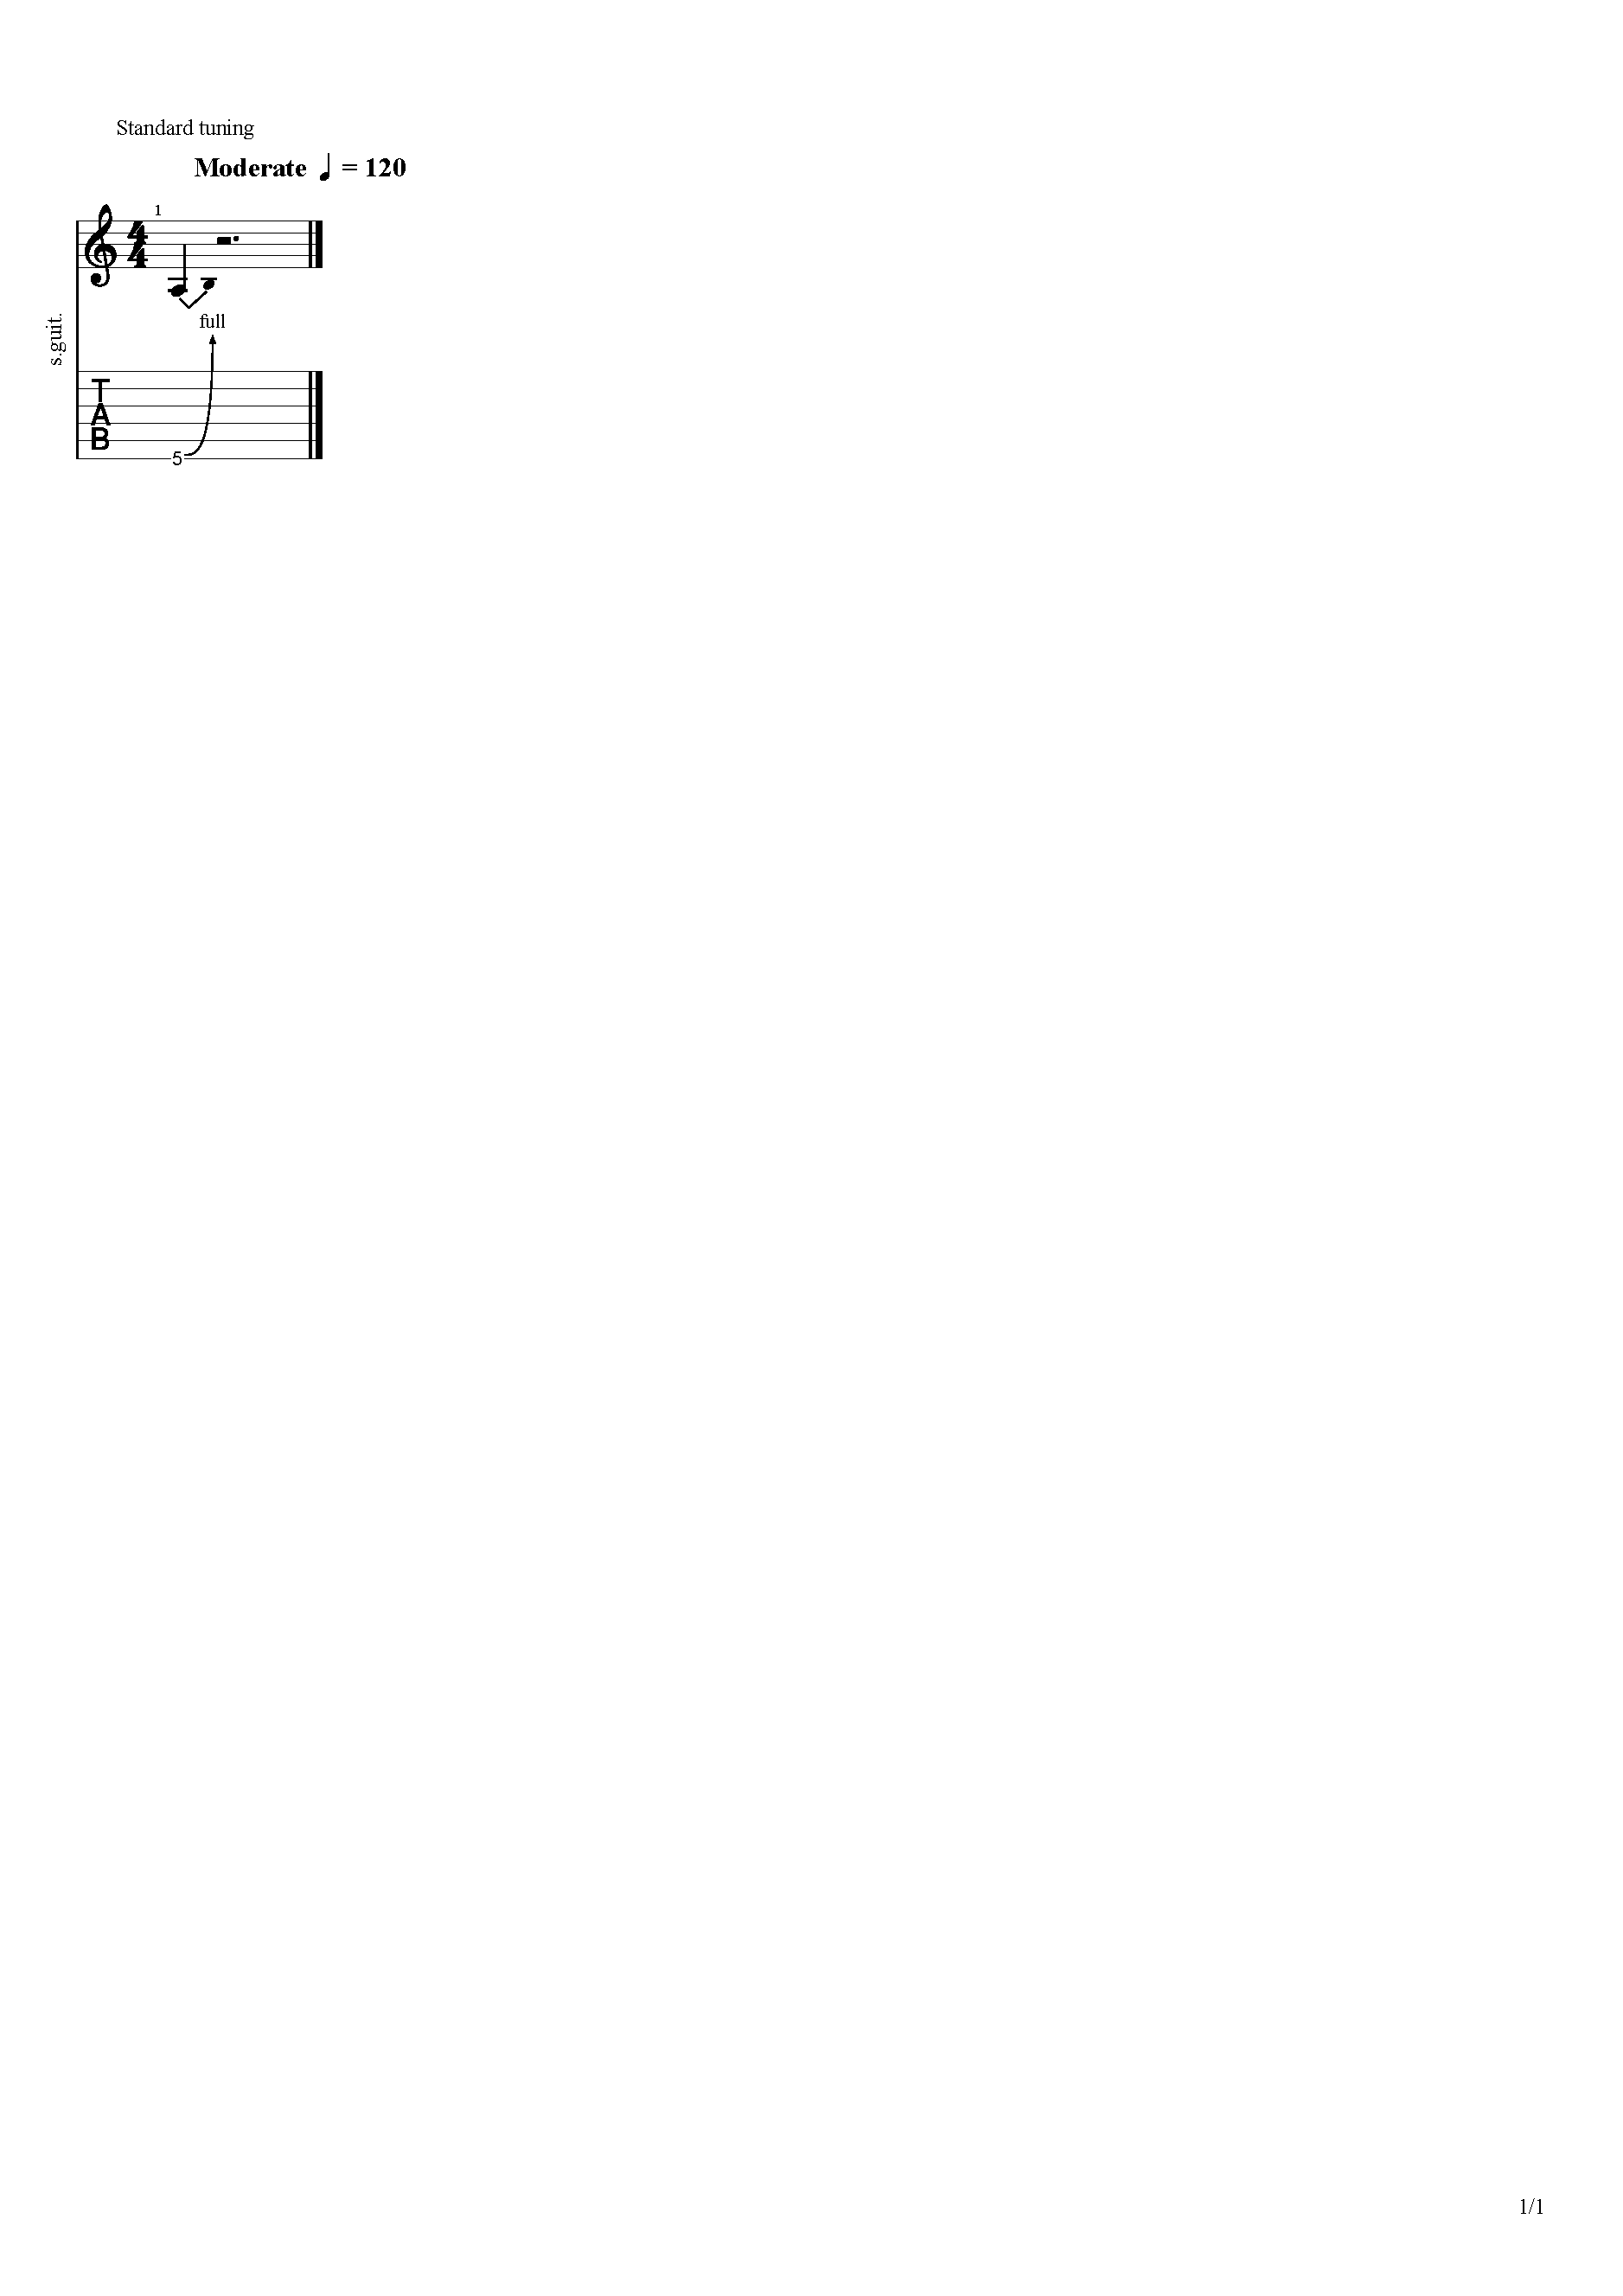
\includegraphics[trim={40 980 690 100}, clip, width=0.135\linewidth]{bend_1.pdf}
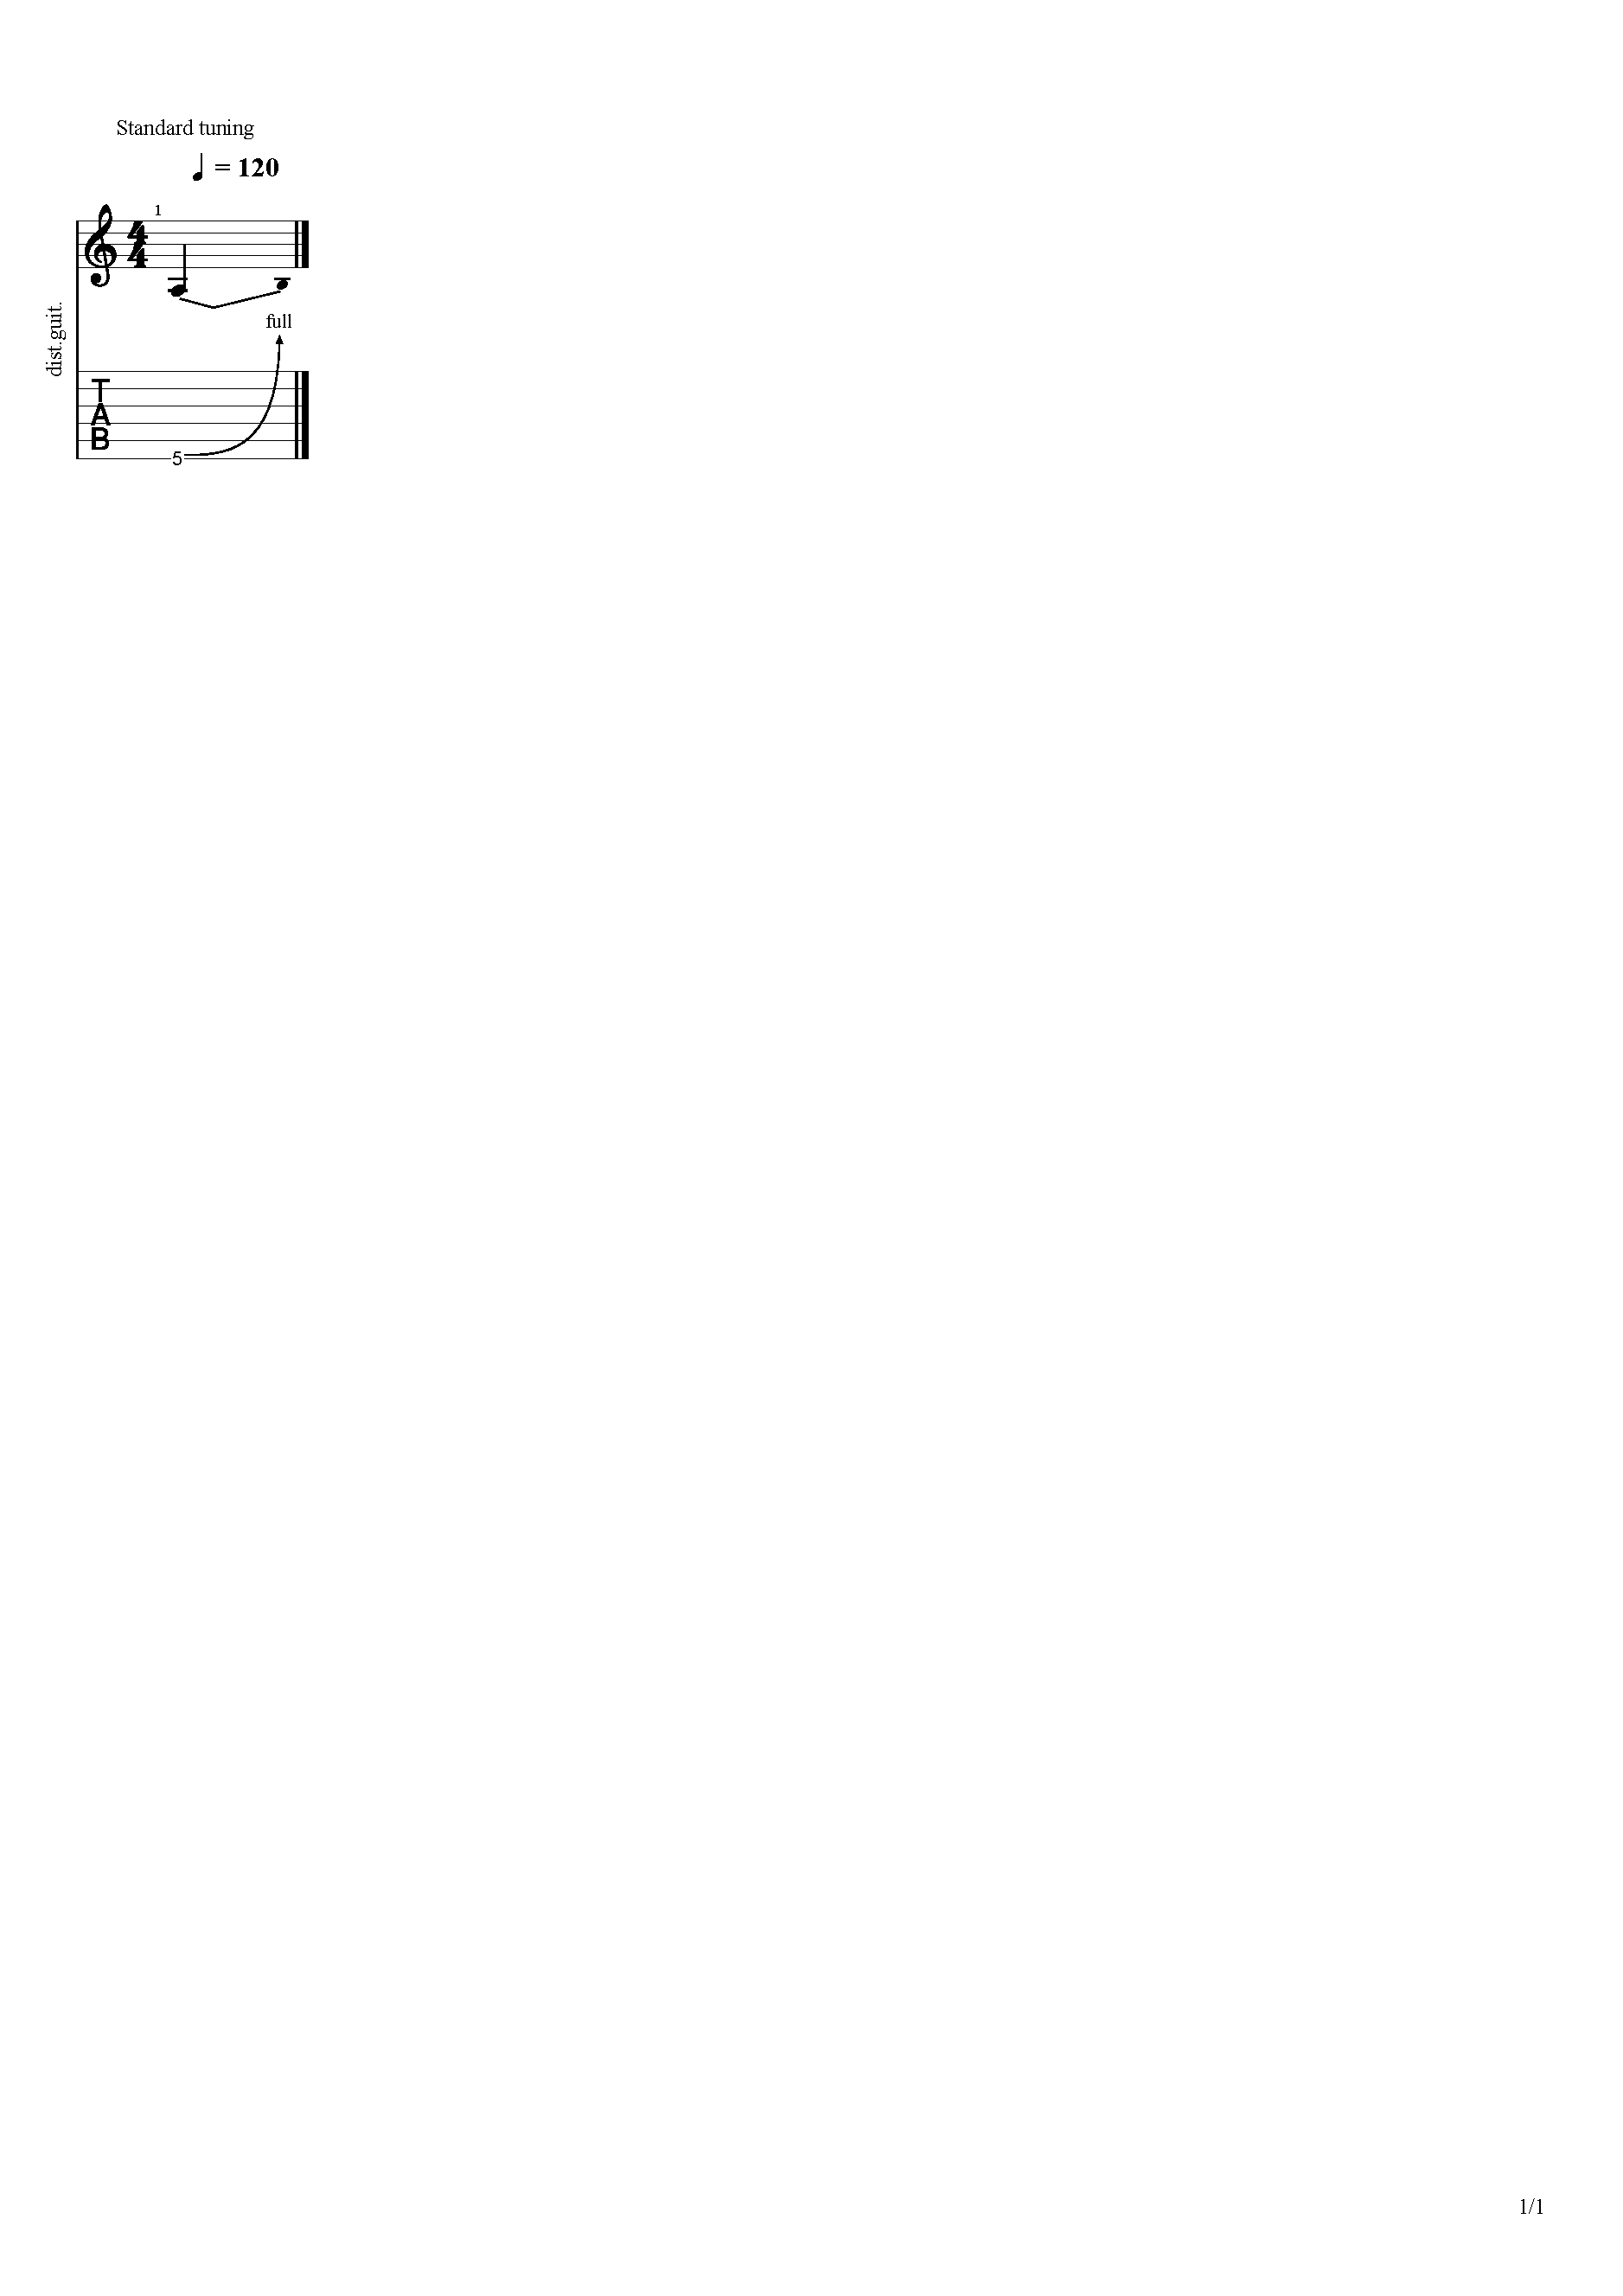
\includegraphics[trim={40 980 690 100}, clip, width=0.135\linewidth]{bend_2.pdf}
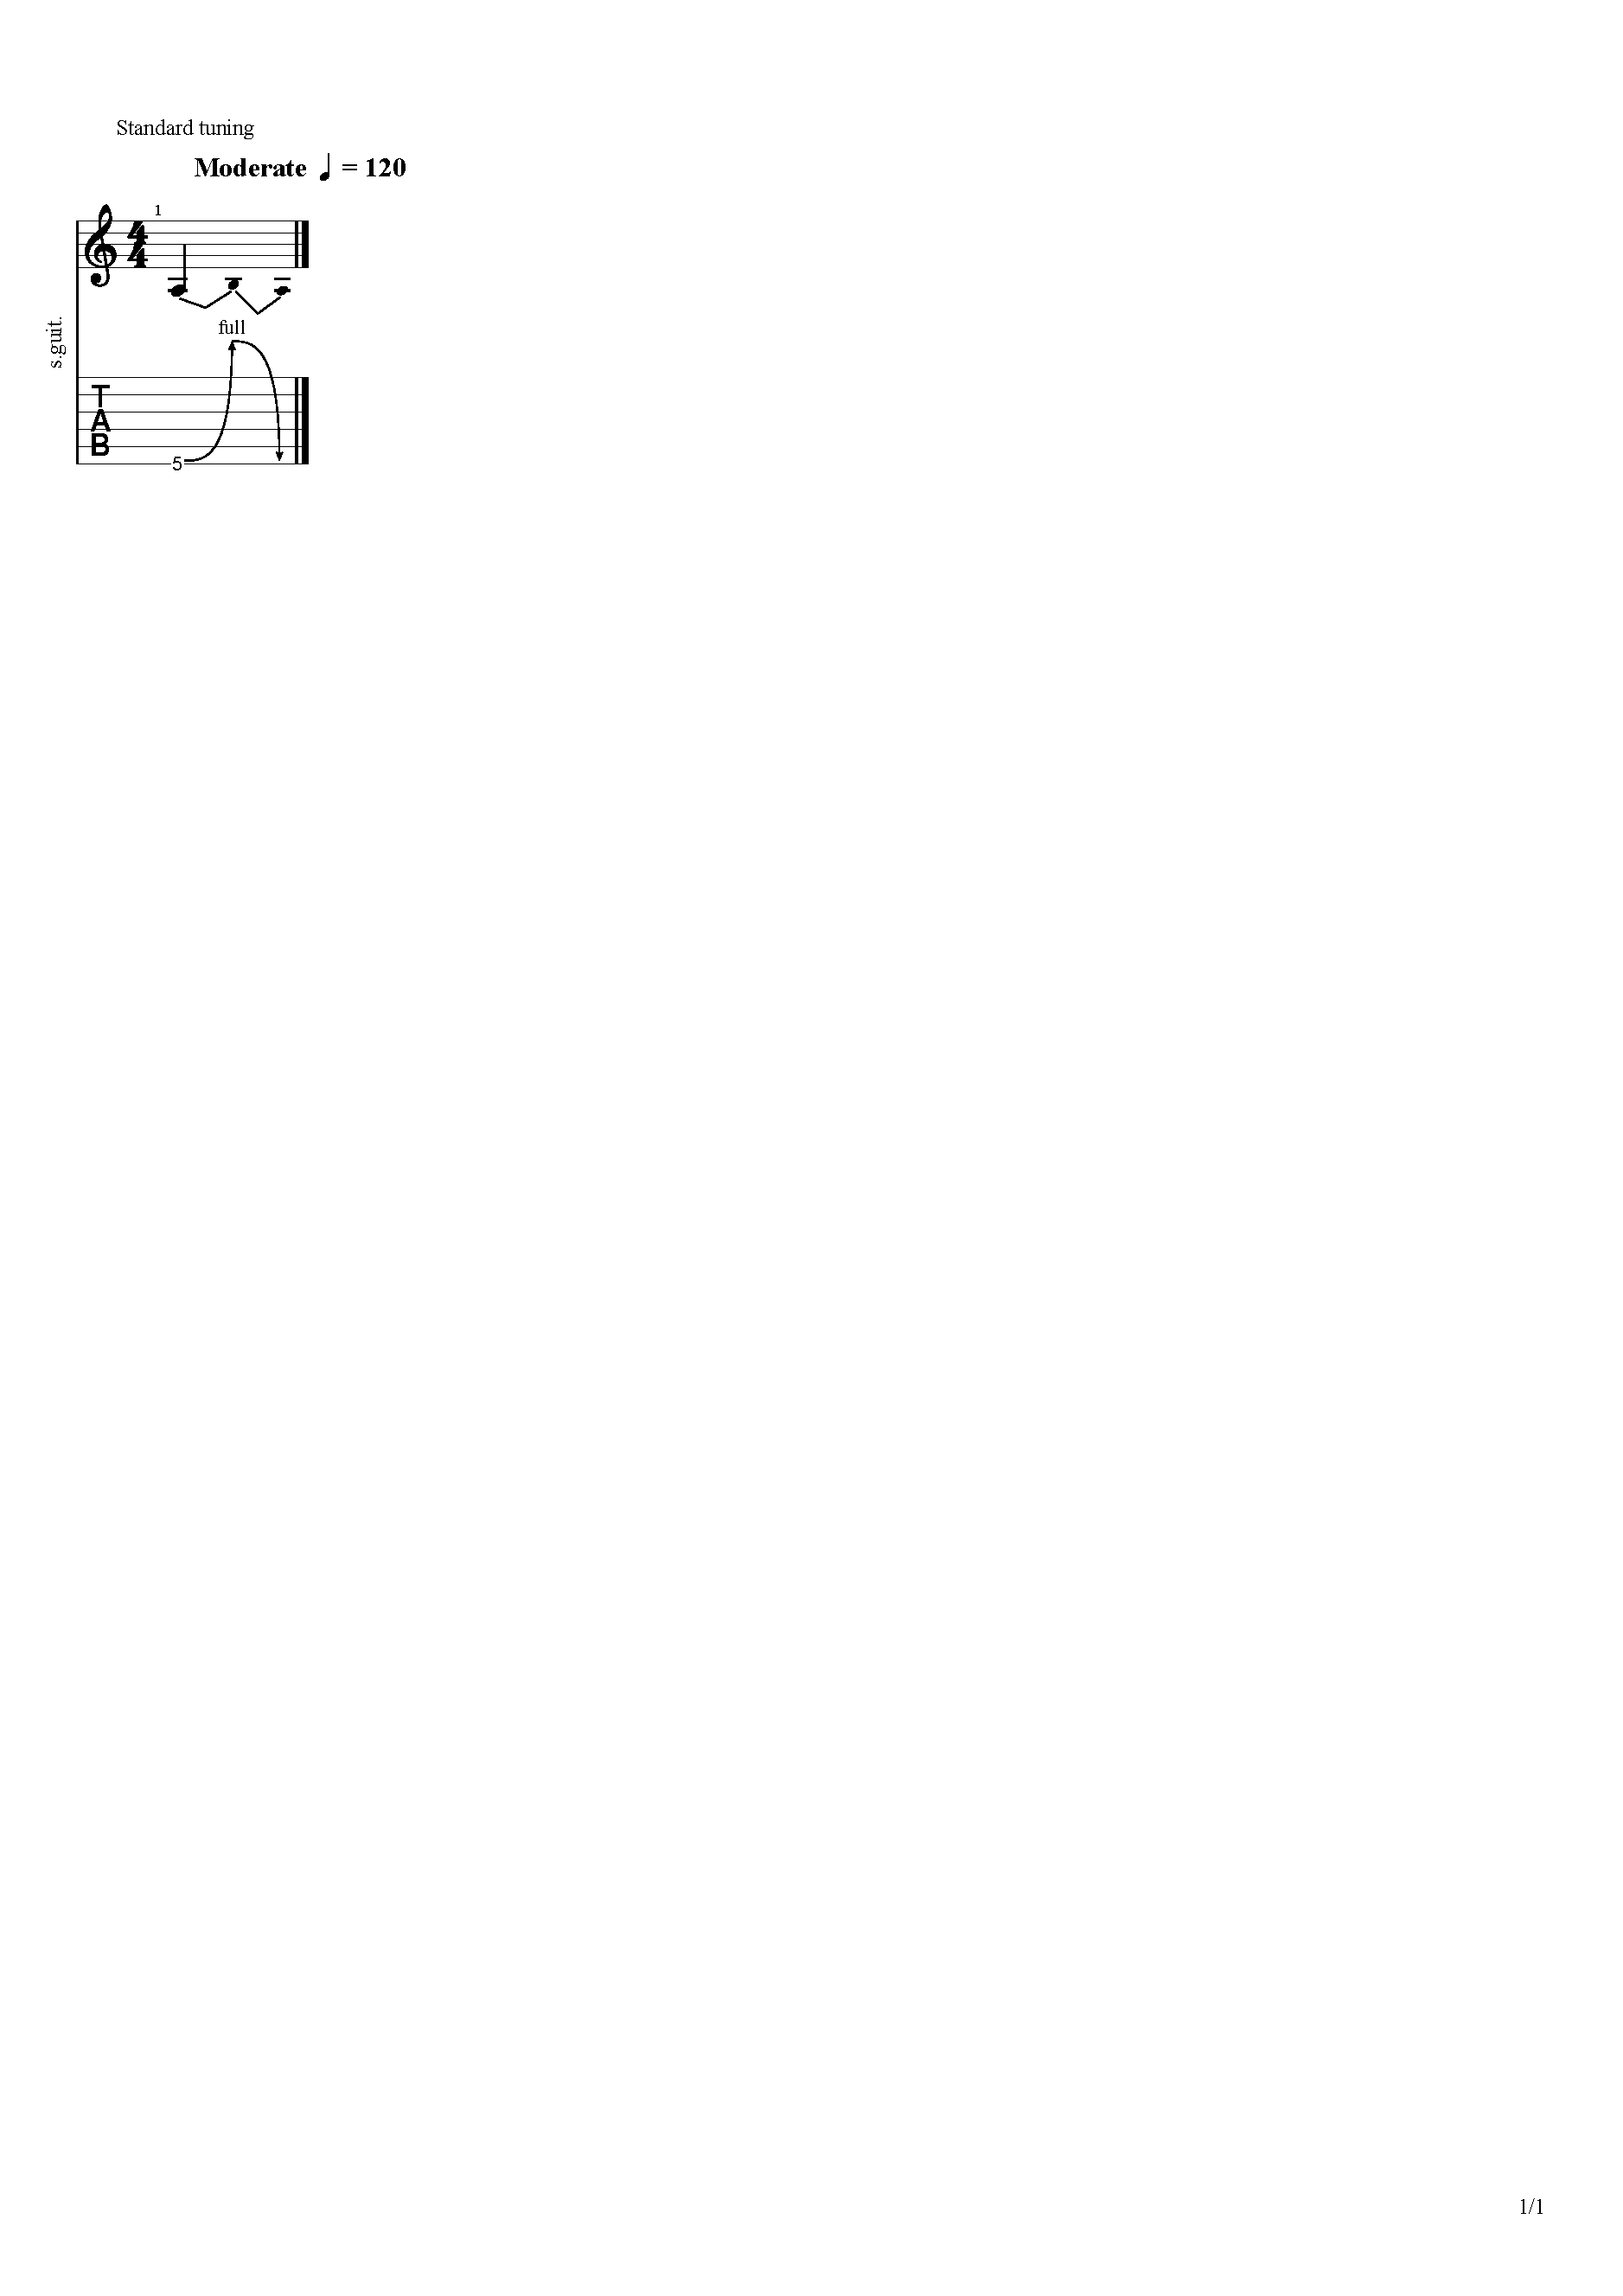
\includegraphics[trim={40 980 690 100}, clip, width=0.135\linewidth]{bend_3.pdf}
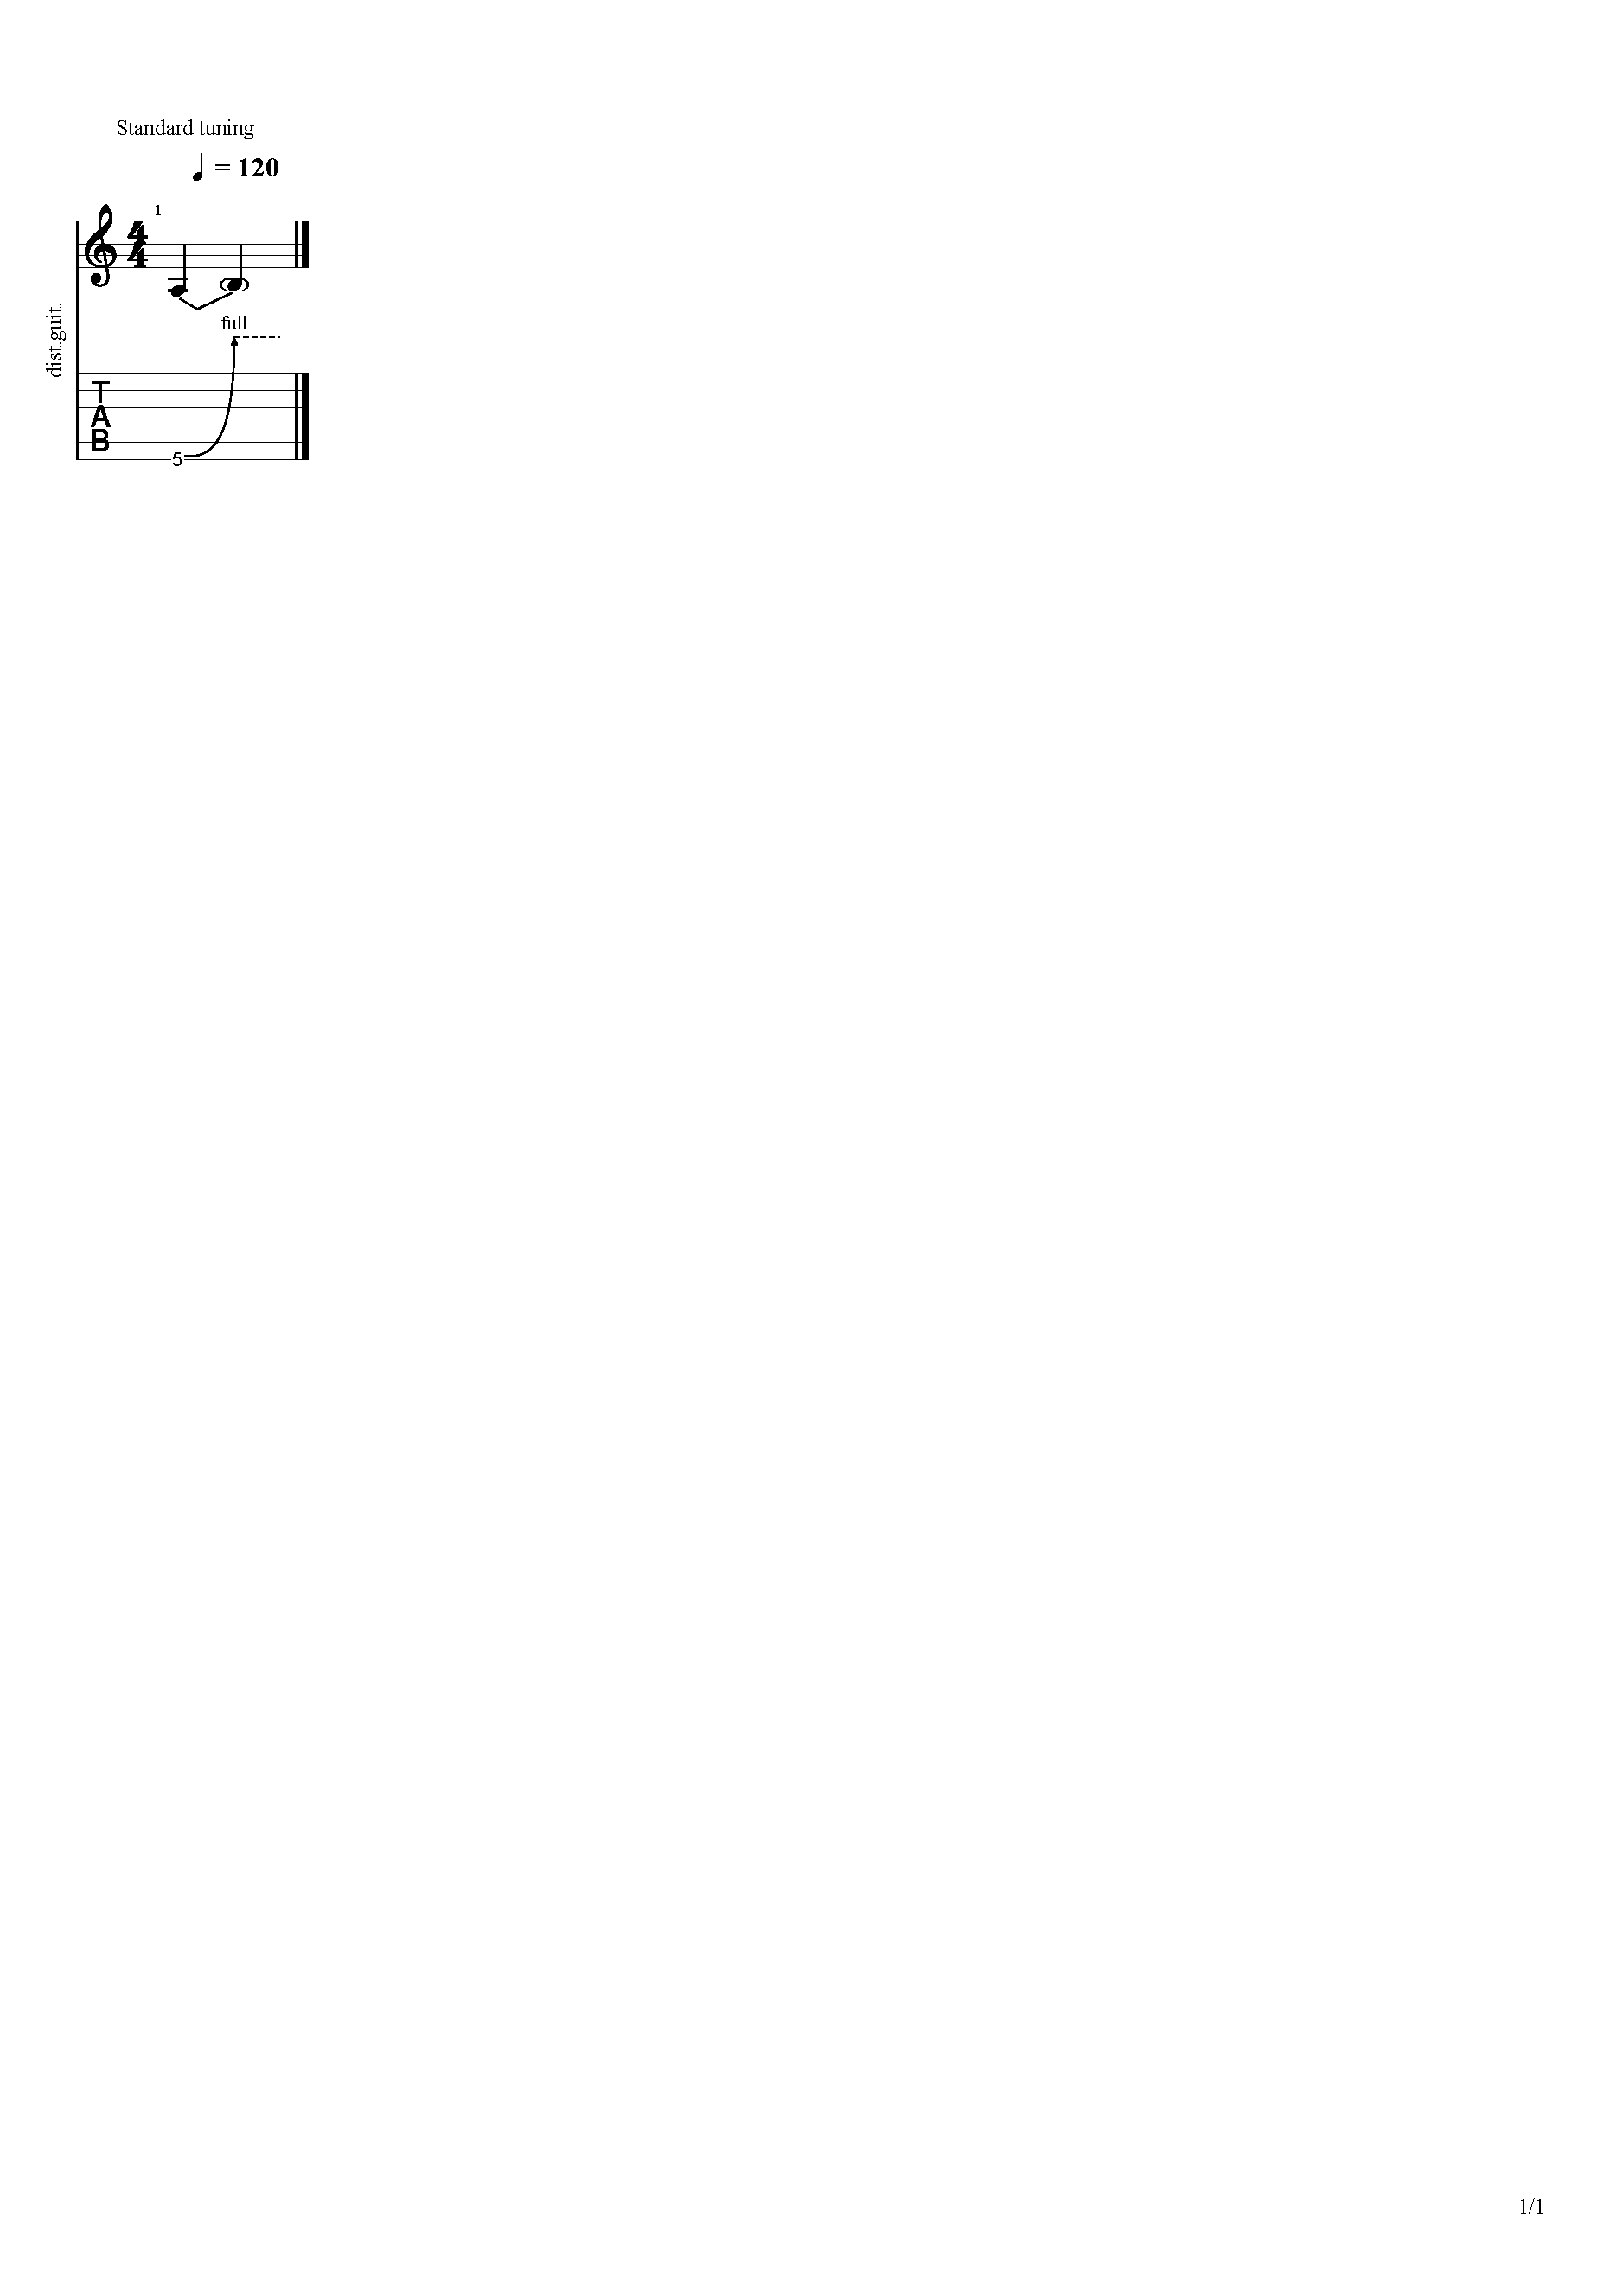
\includegraphics[trim={40 980 690 100}, clip, width=0.135\linewidth]{bend_4.pdf}
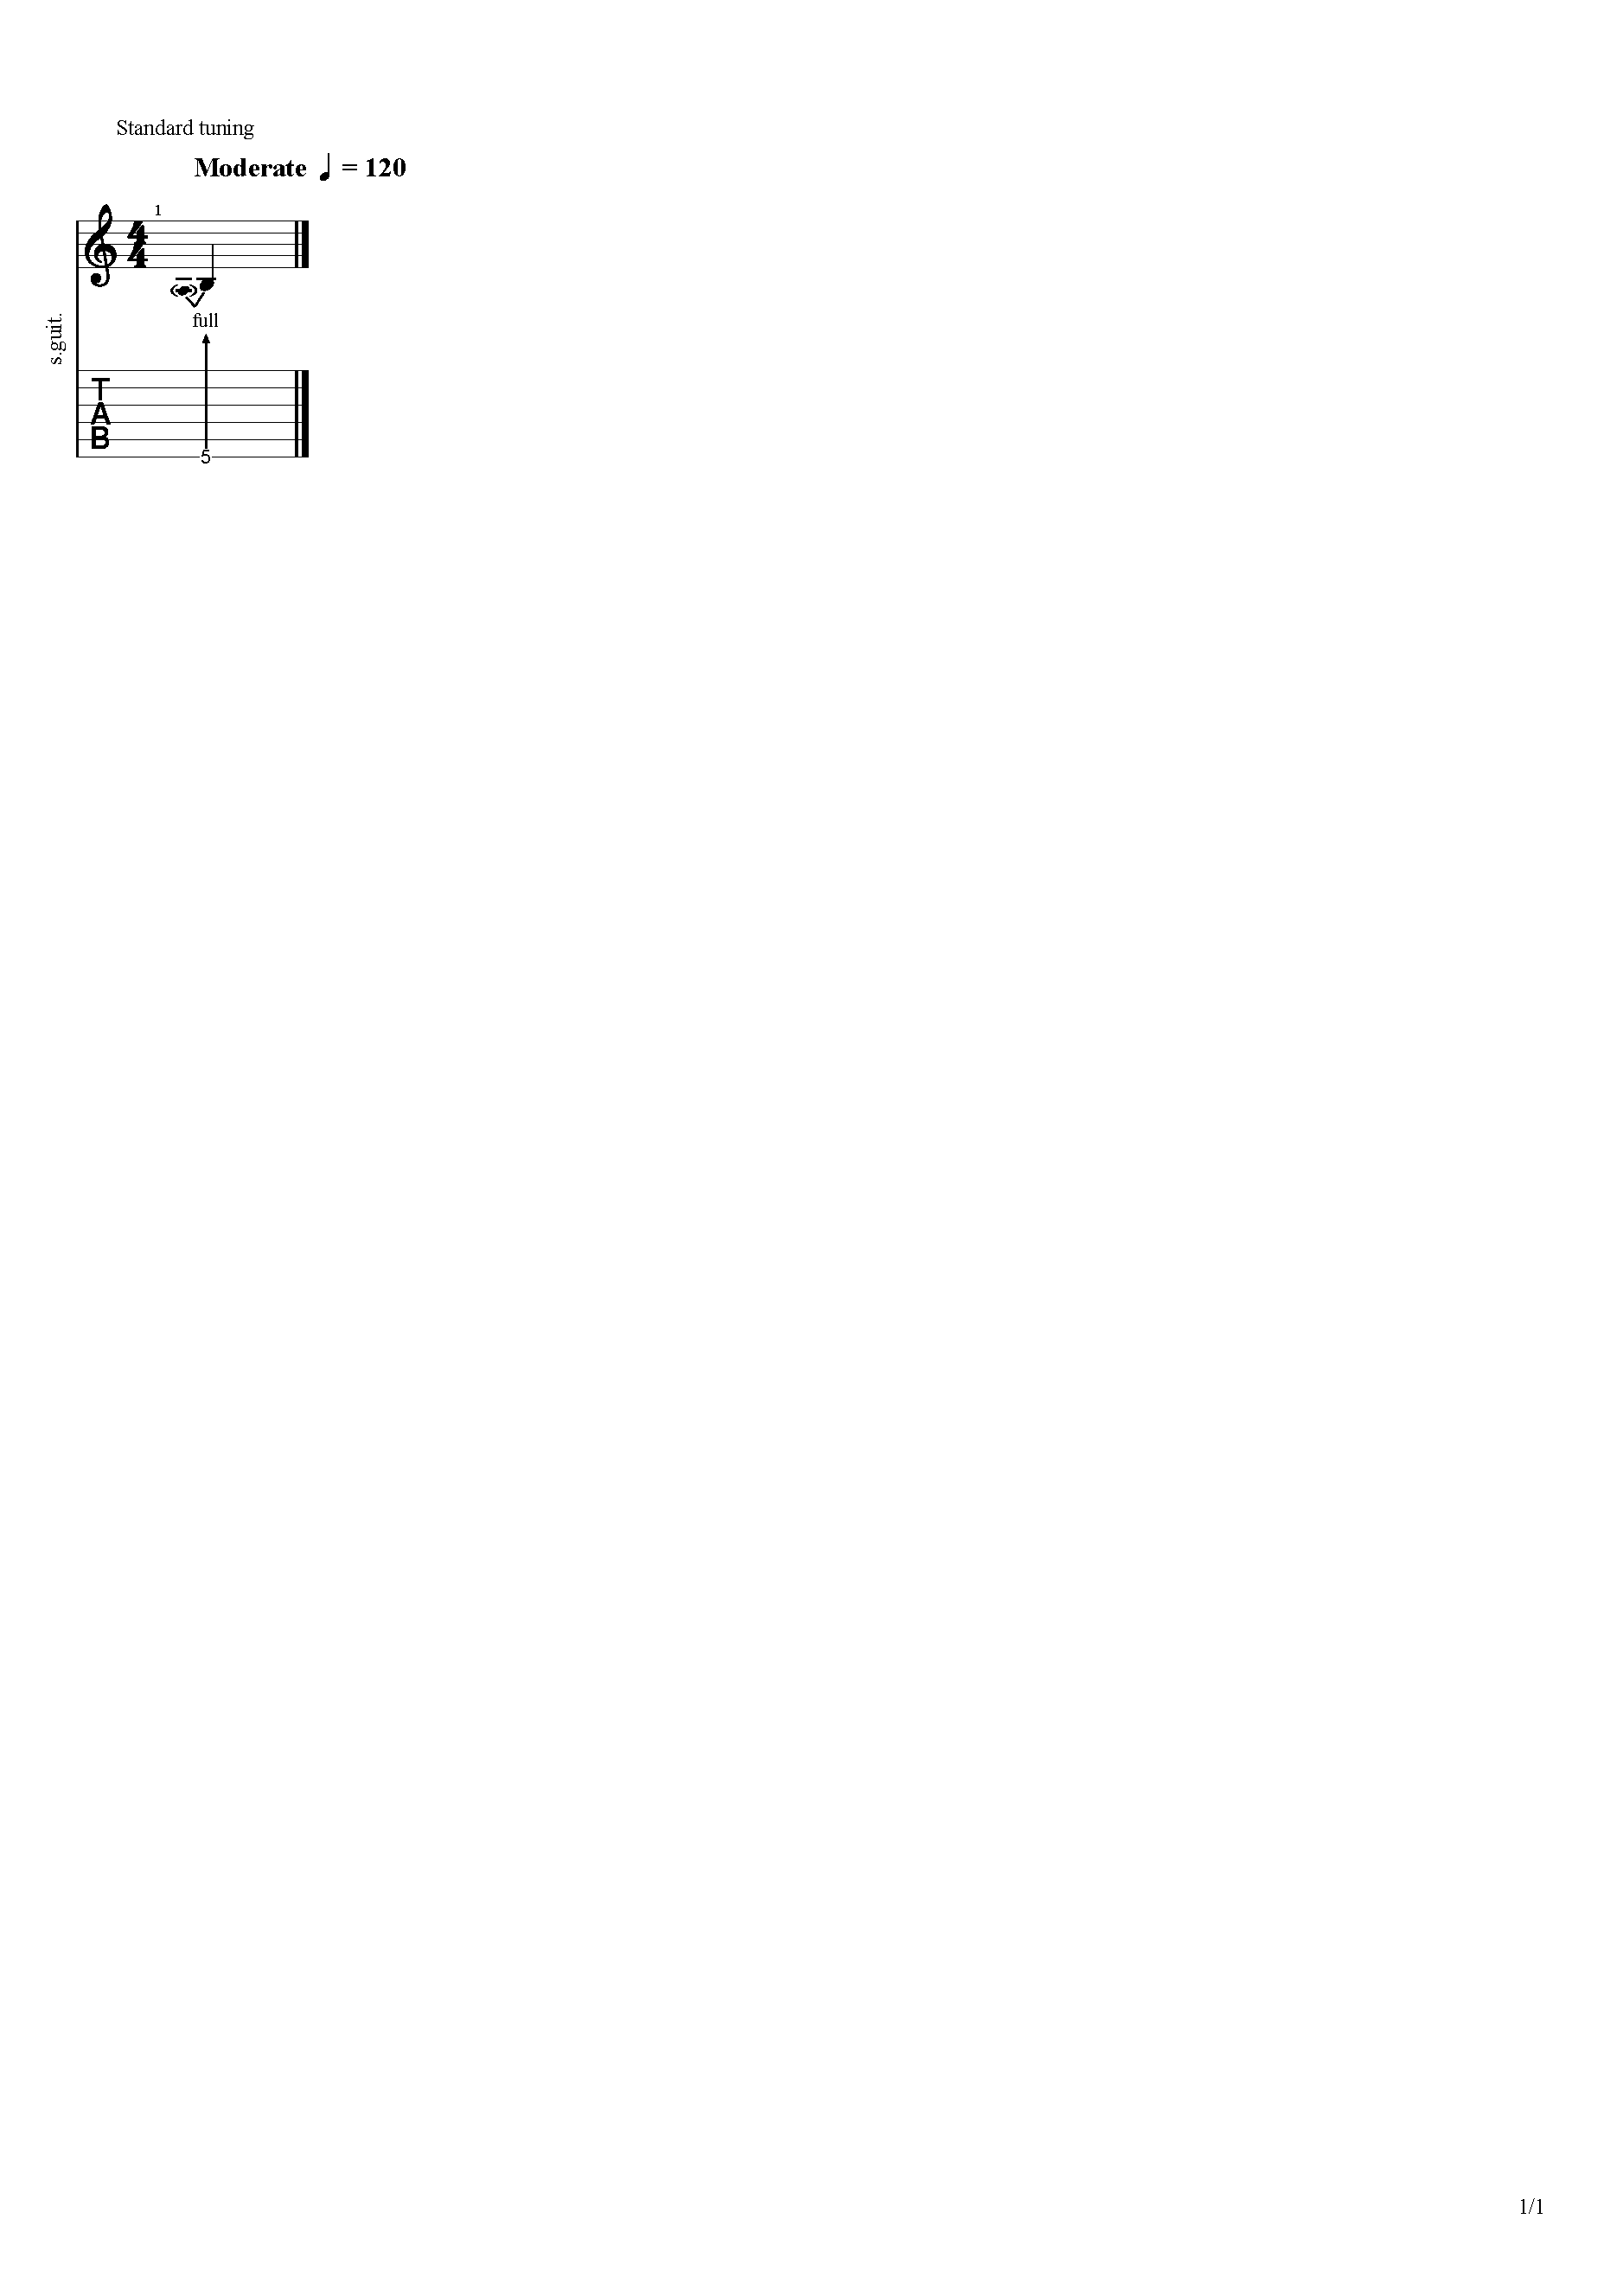
\includegraphics[trim={40 980 690 100}, clip, width=0.135\linewidth]{bend_5.pdf}
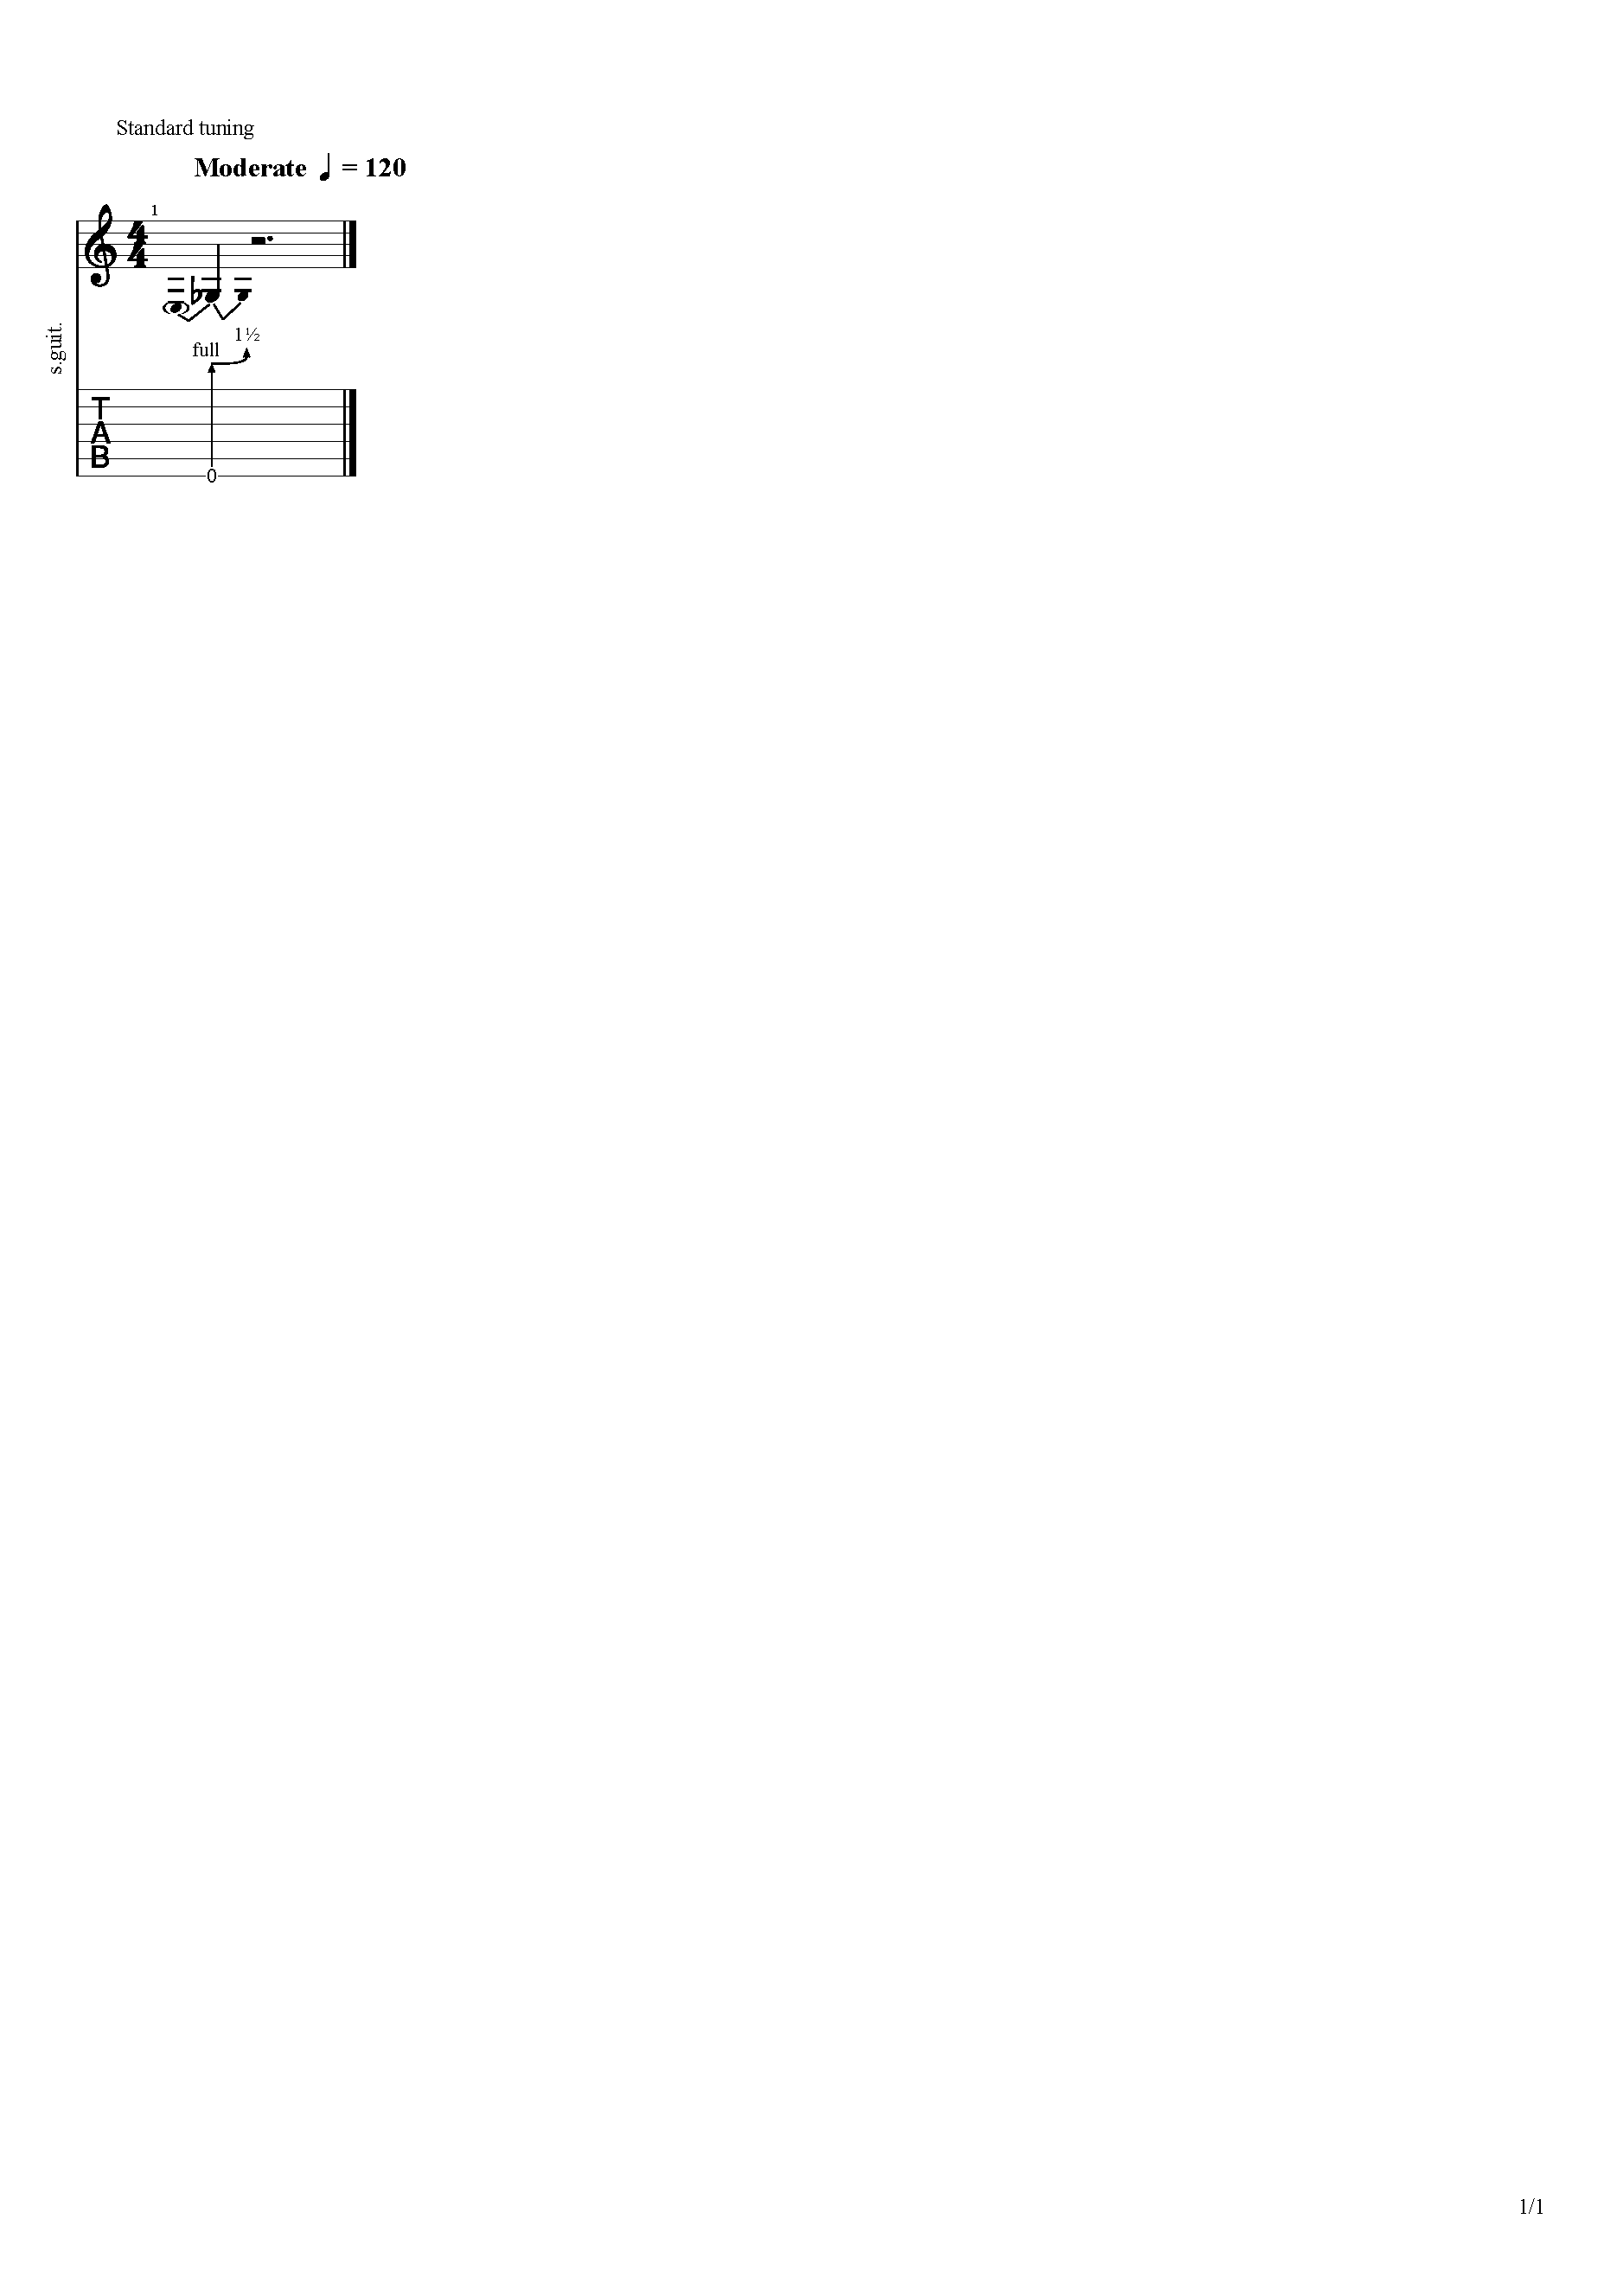
\includegraphics[trim={40 980 690 100}, clip, width=0.135\linewidth]{bend_6.pdf}
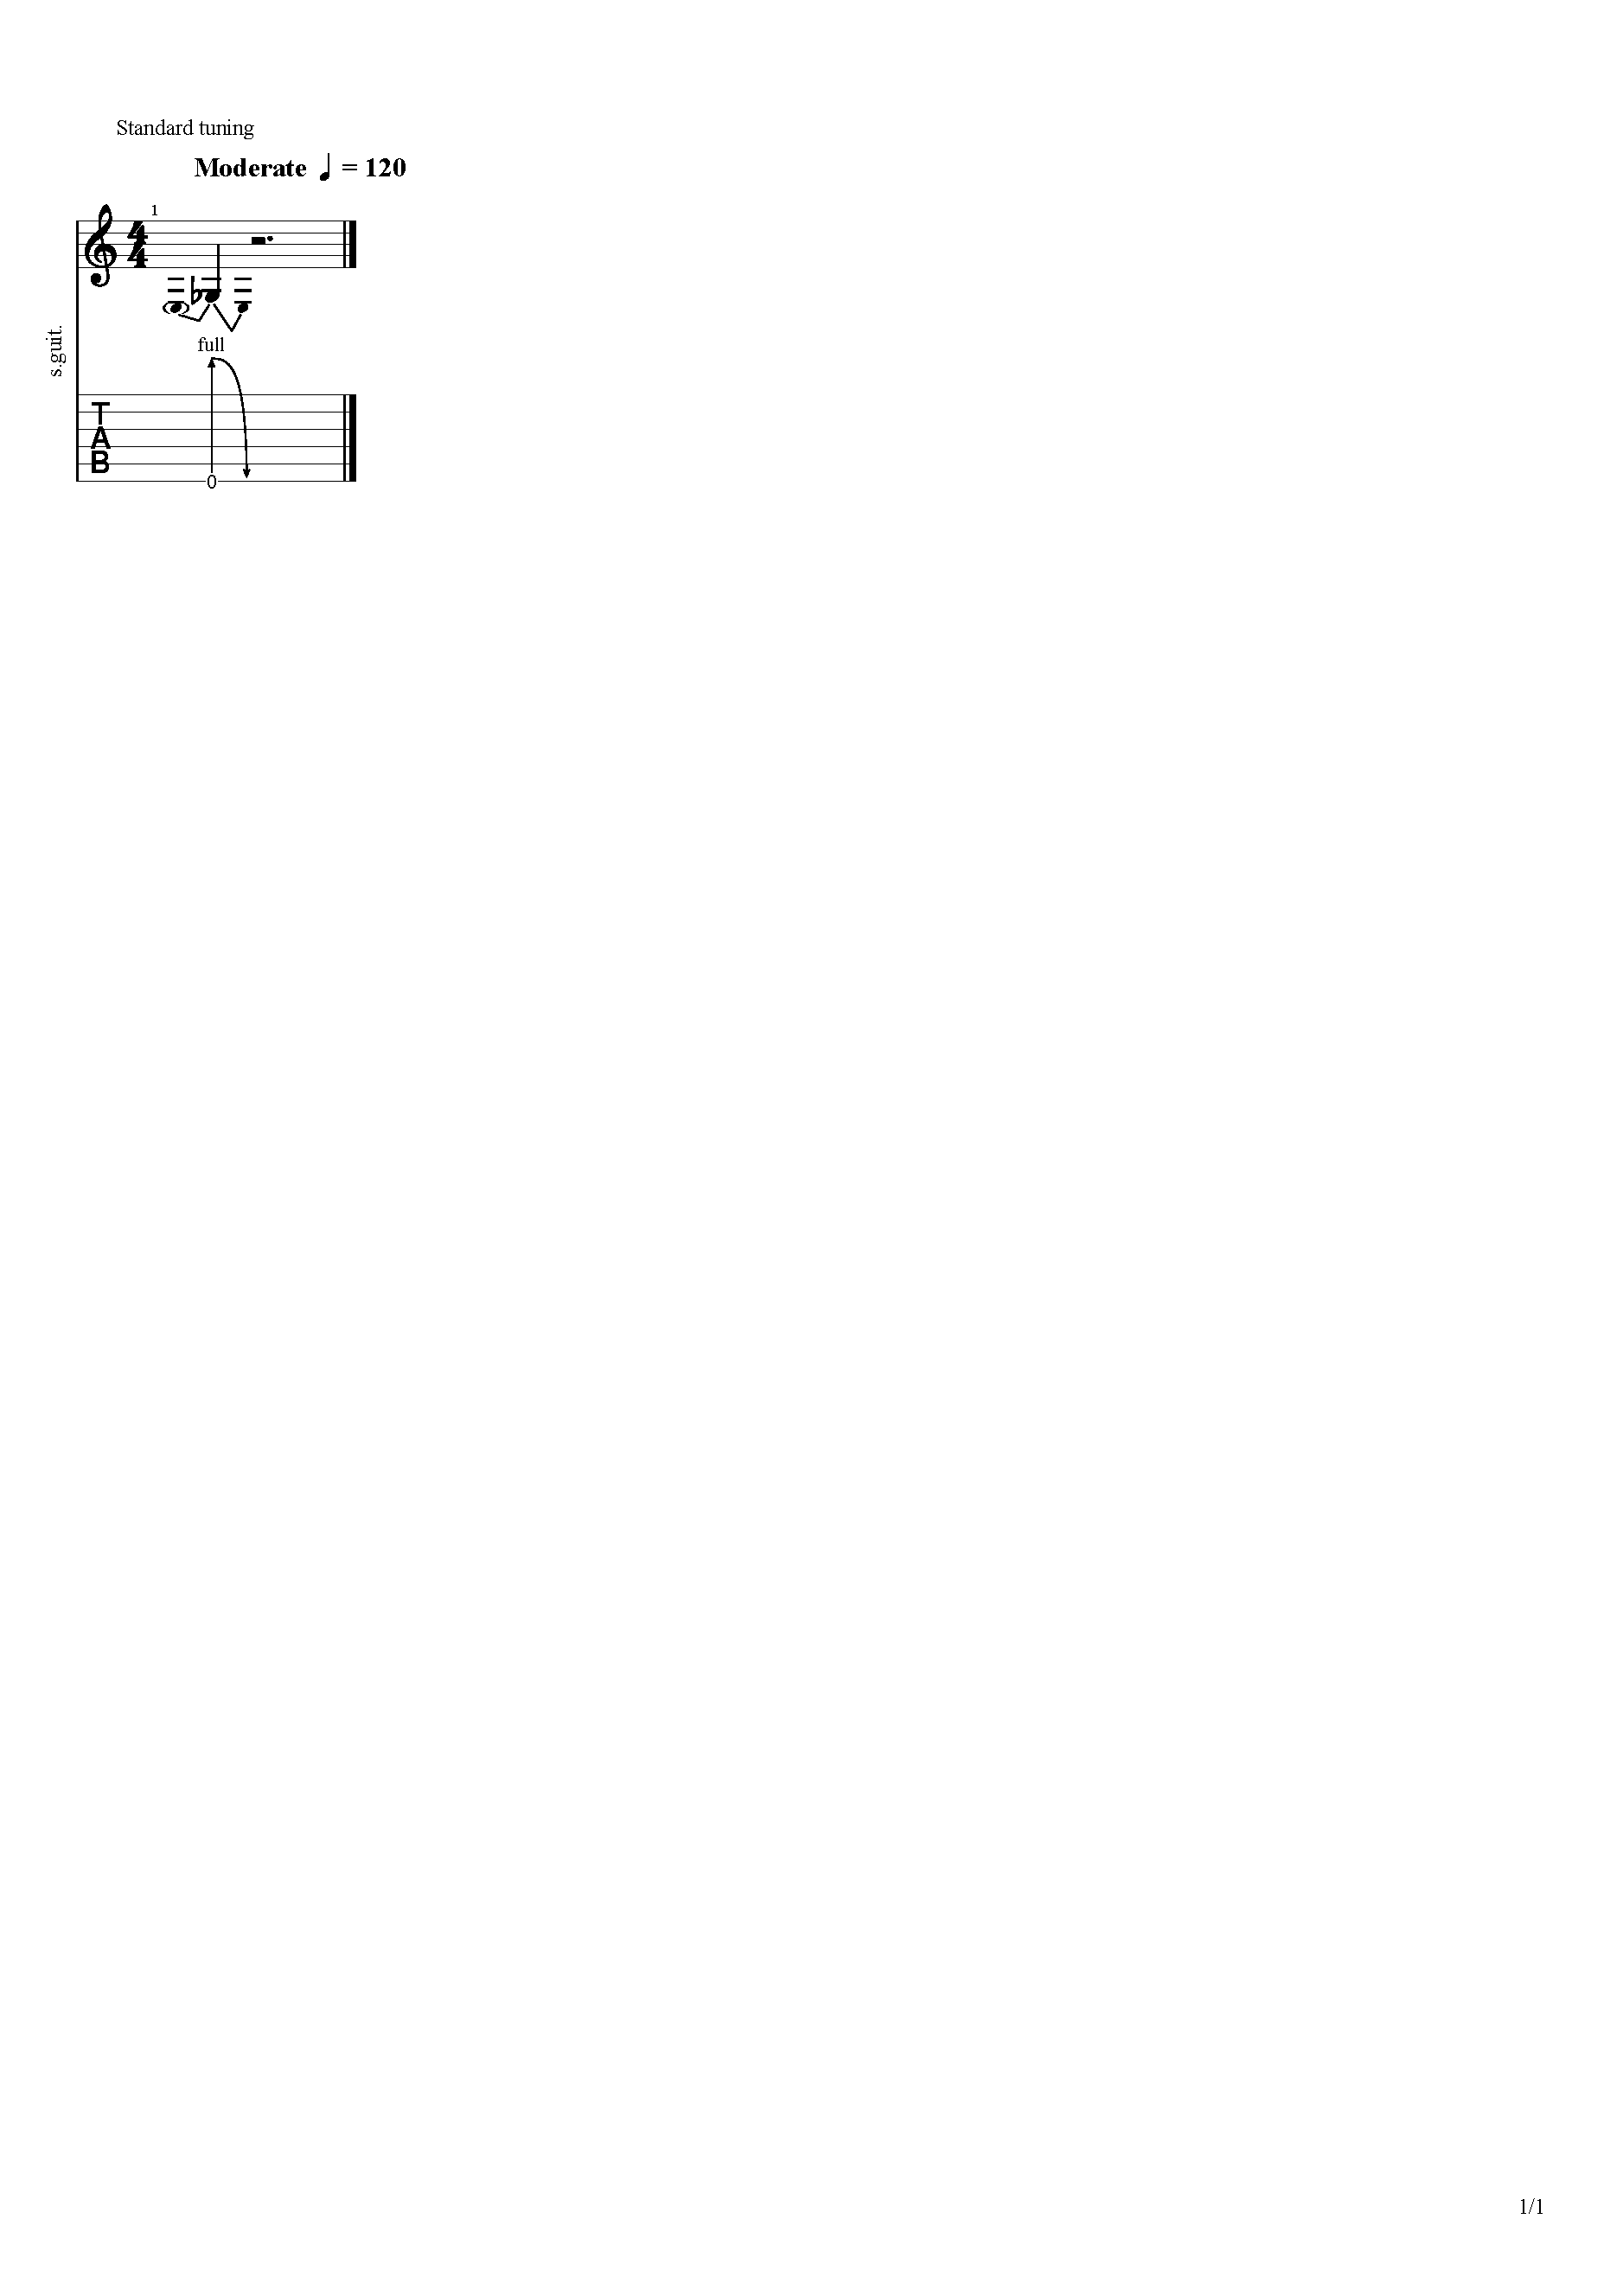
\includegraphics[trim={40 980 690 100}, clip, width=0.135\linewidth]{bend_7.pdf}
\caption{Bend types and their pitch variations.}
  \label{fig:bend}
\end{figure}
\subsubsection{Tremolo bar}
A tremolo bar or whammy bar is a device attached to the bridge of a guitar that 
allows bending the pitch of notes by pushing or pulling on the bar.
\begin{figure}[htbp]
  \centering
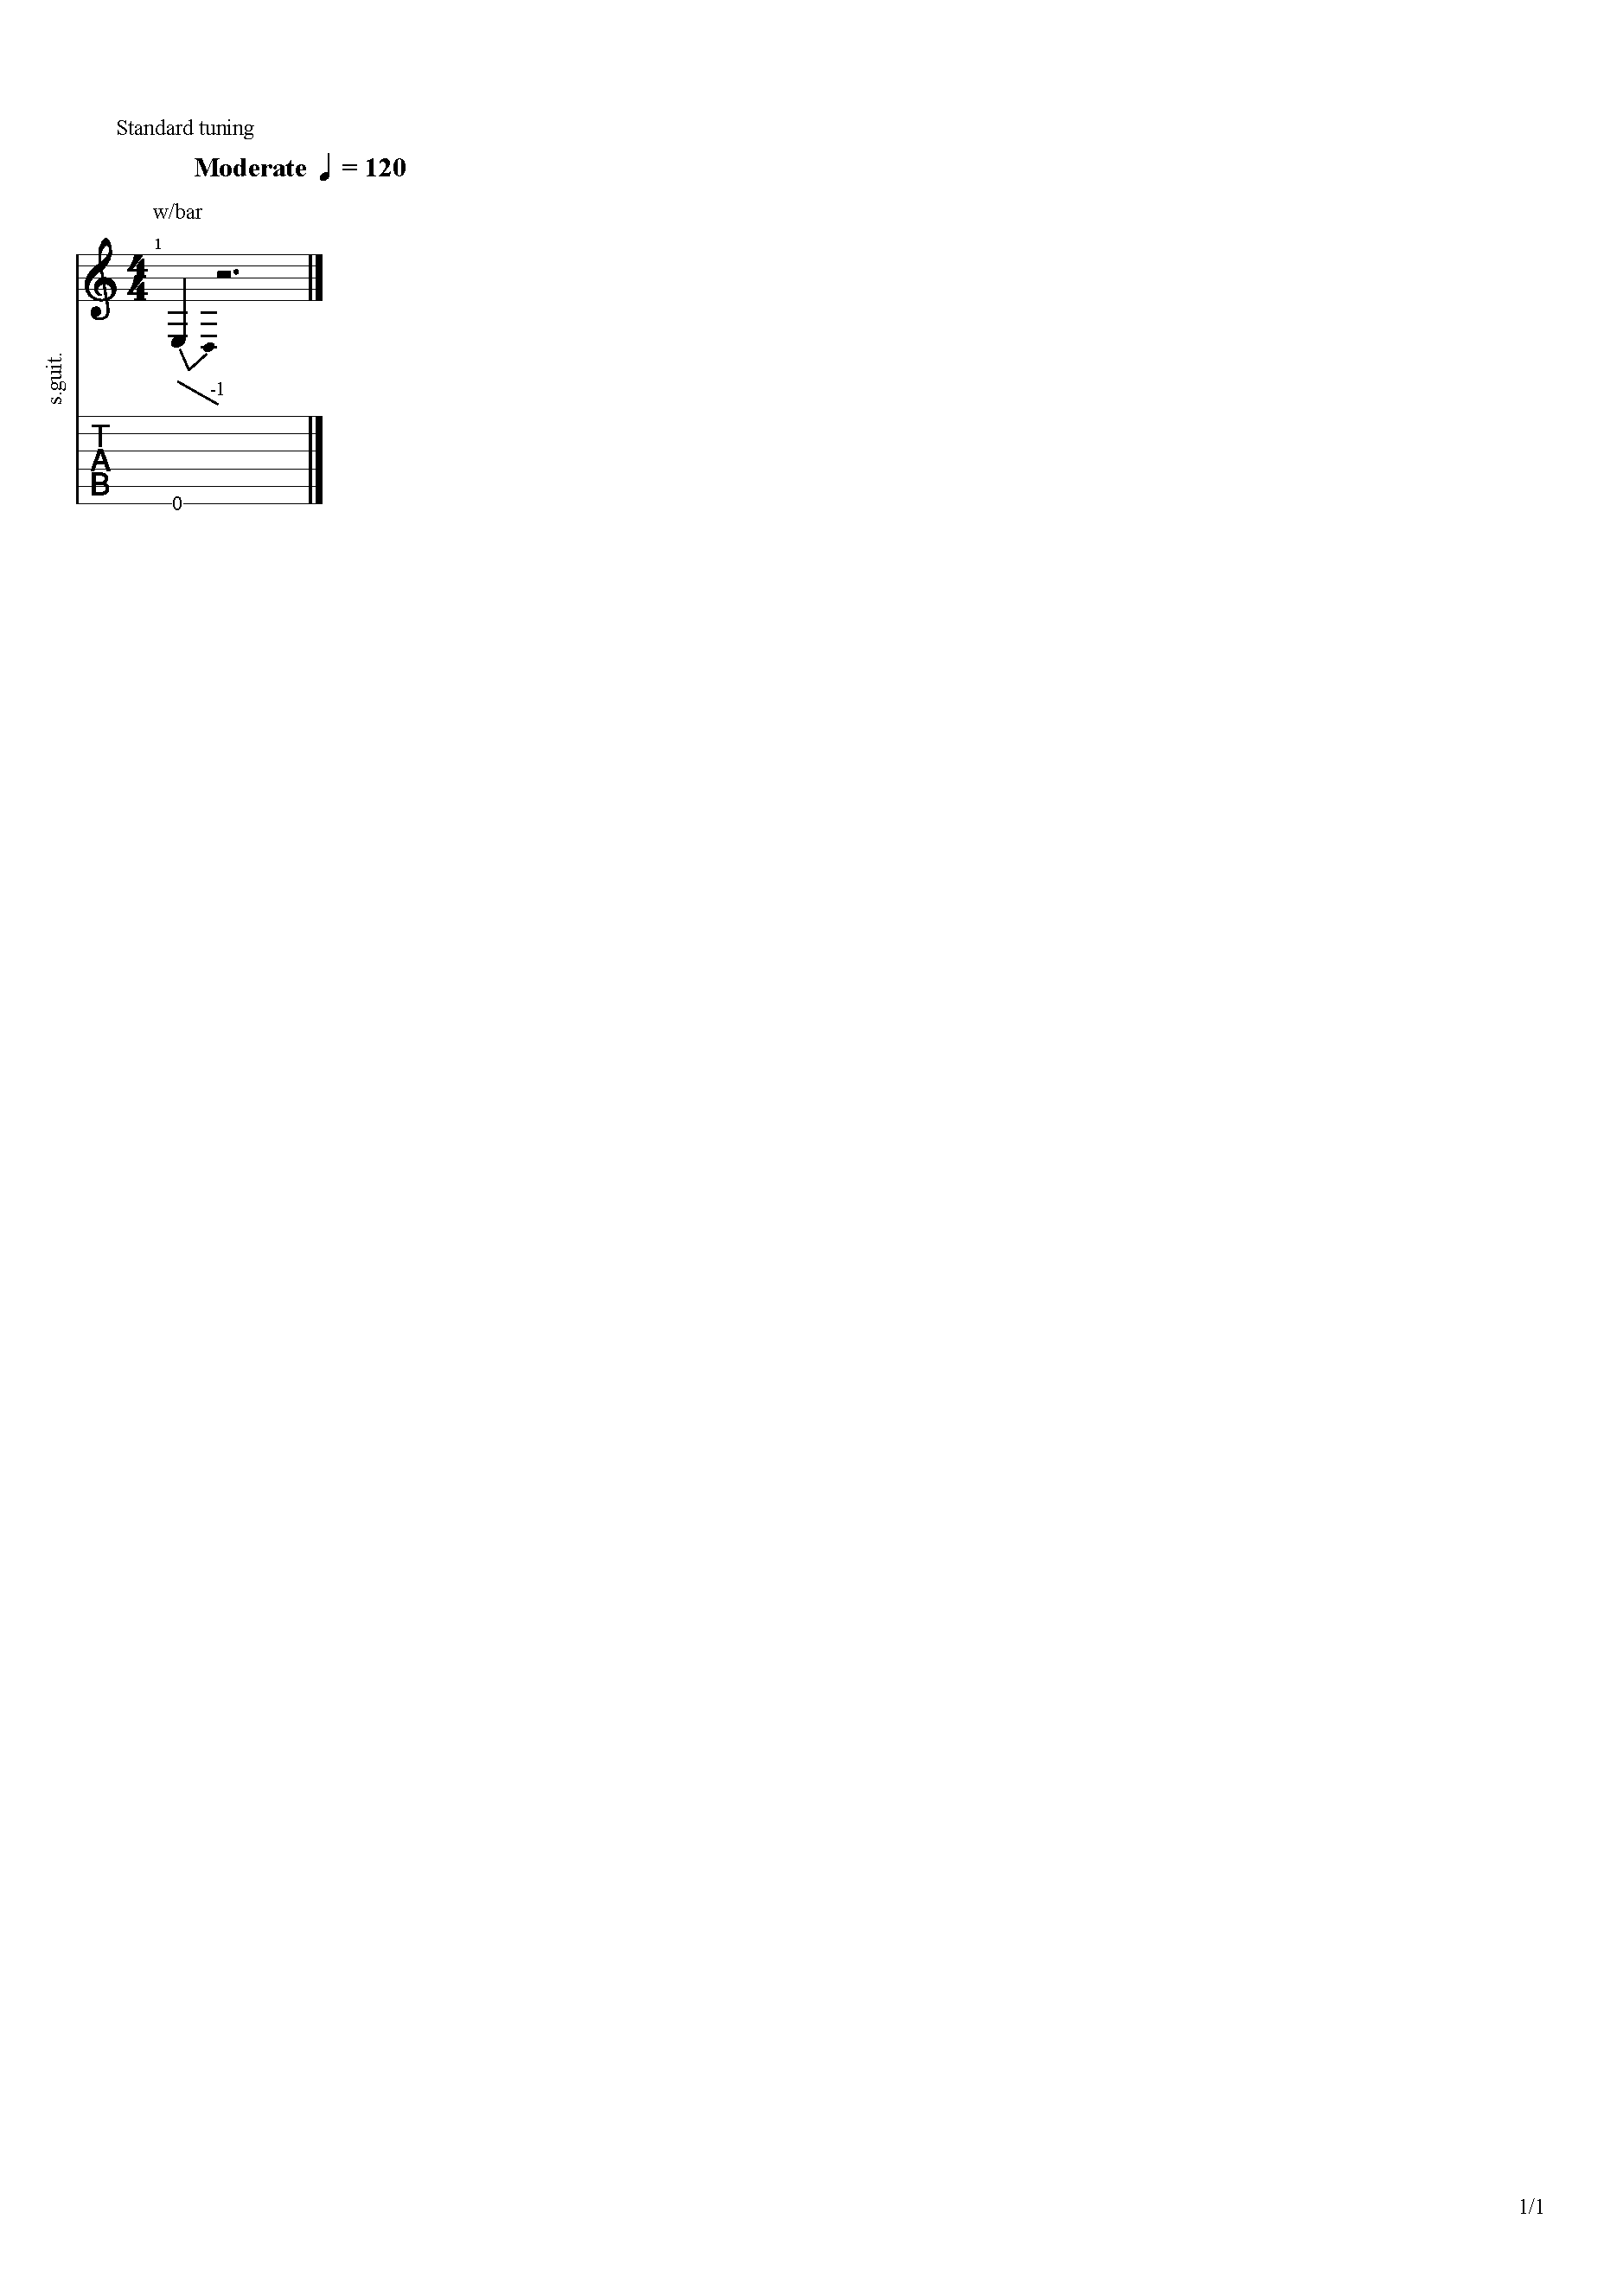
\includegraphics[trim={40 980 690 100}, clip, width=0.195\linewidth]{trem_1.pdf}
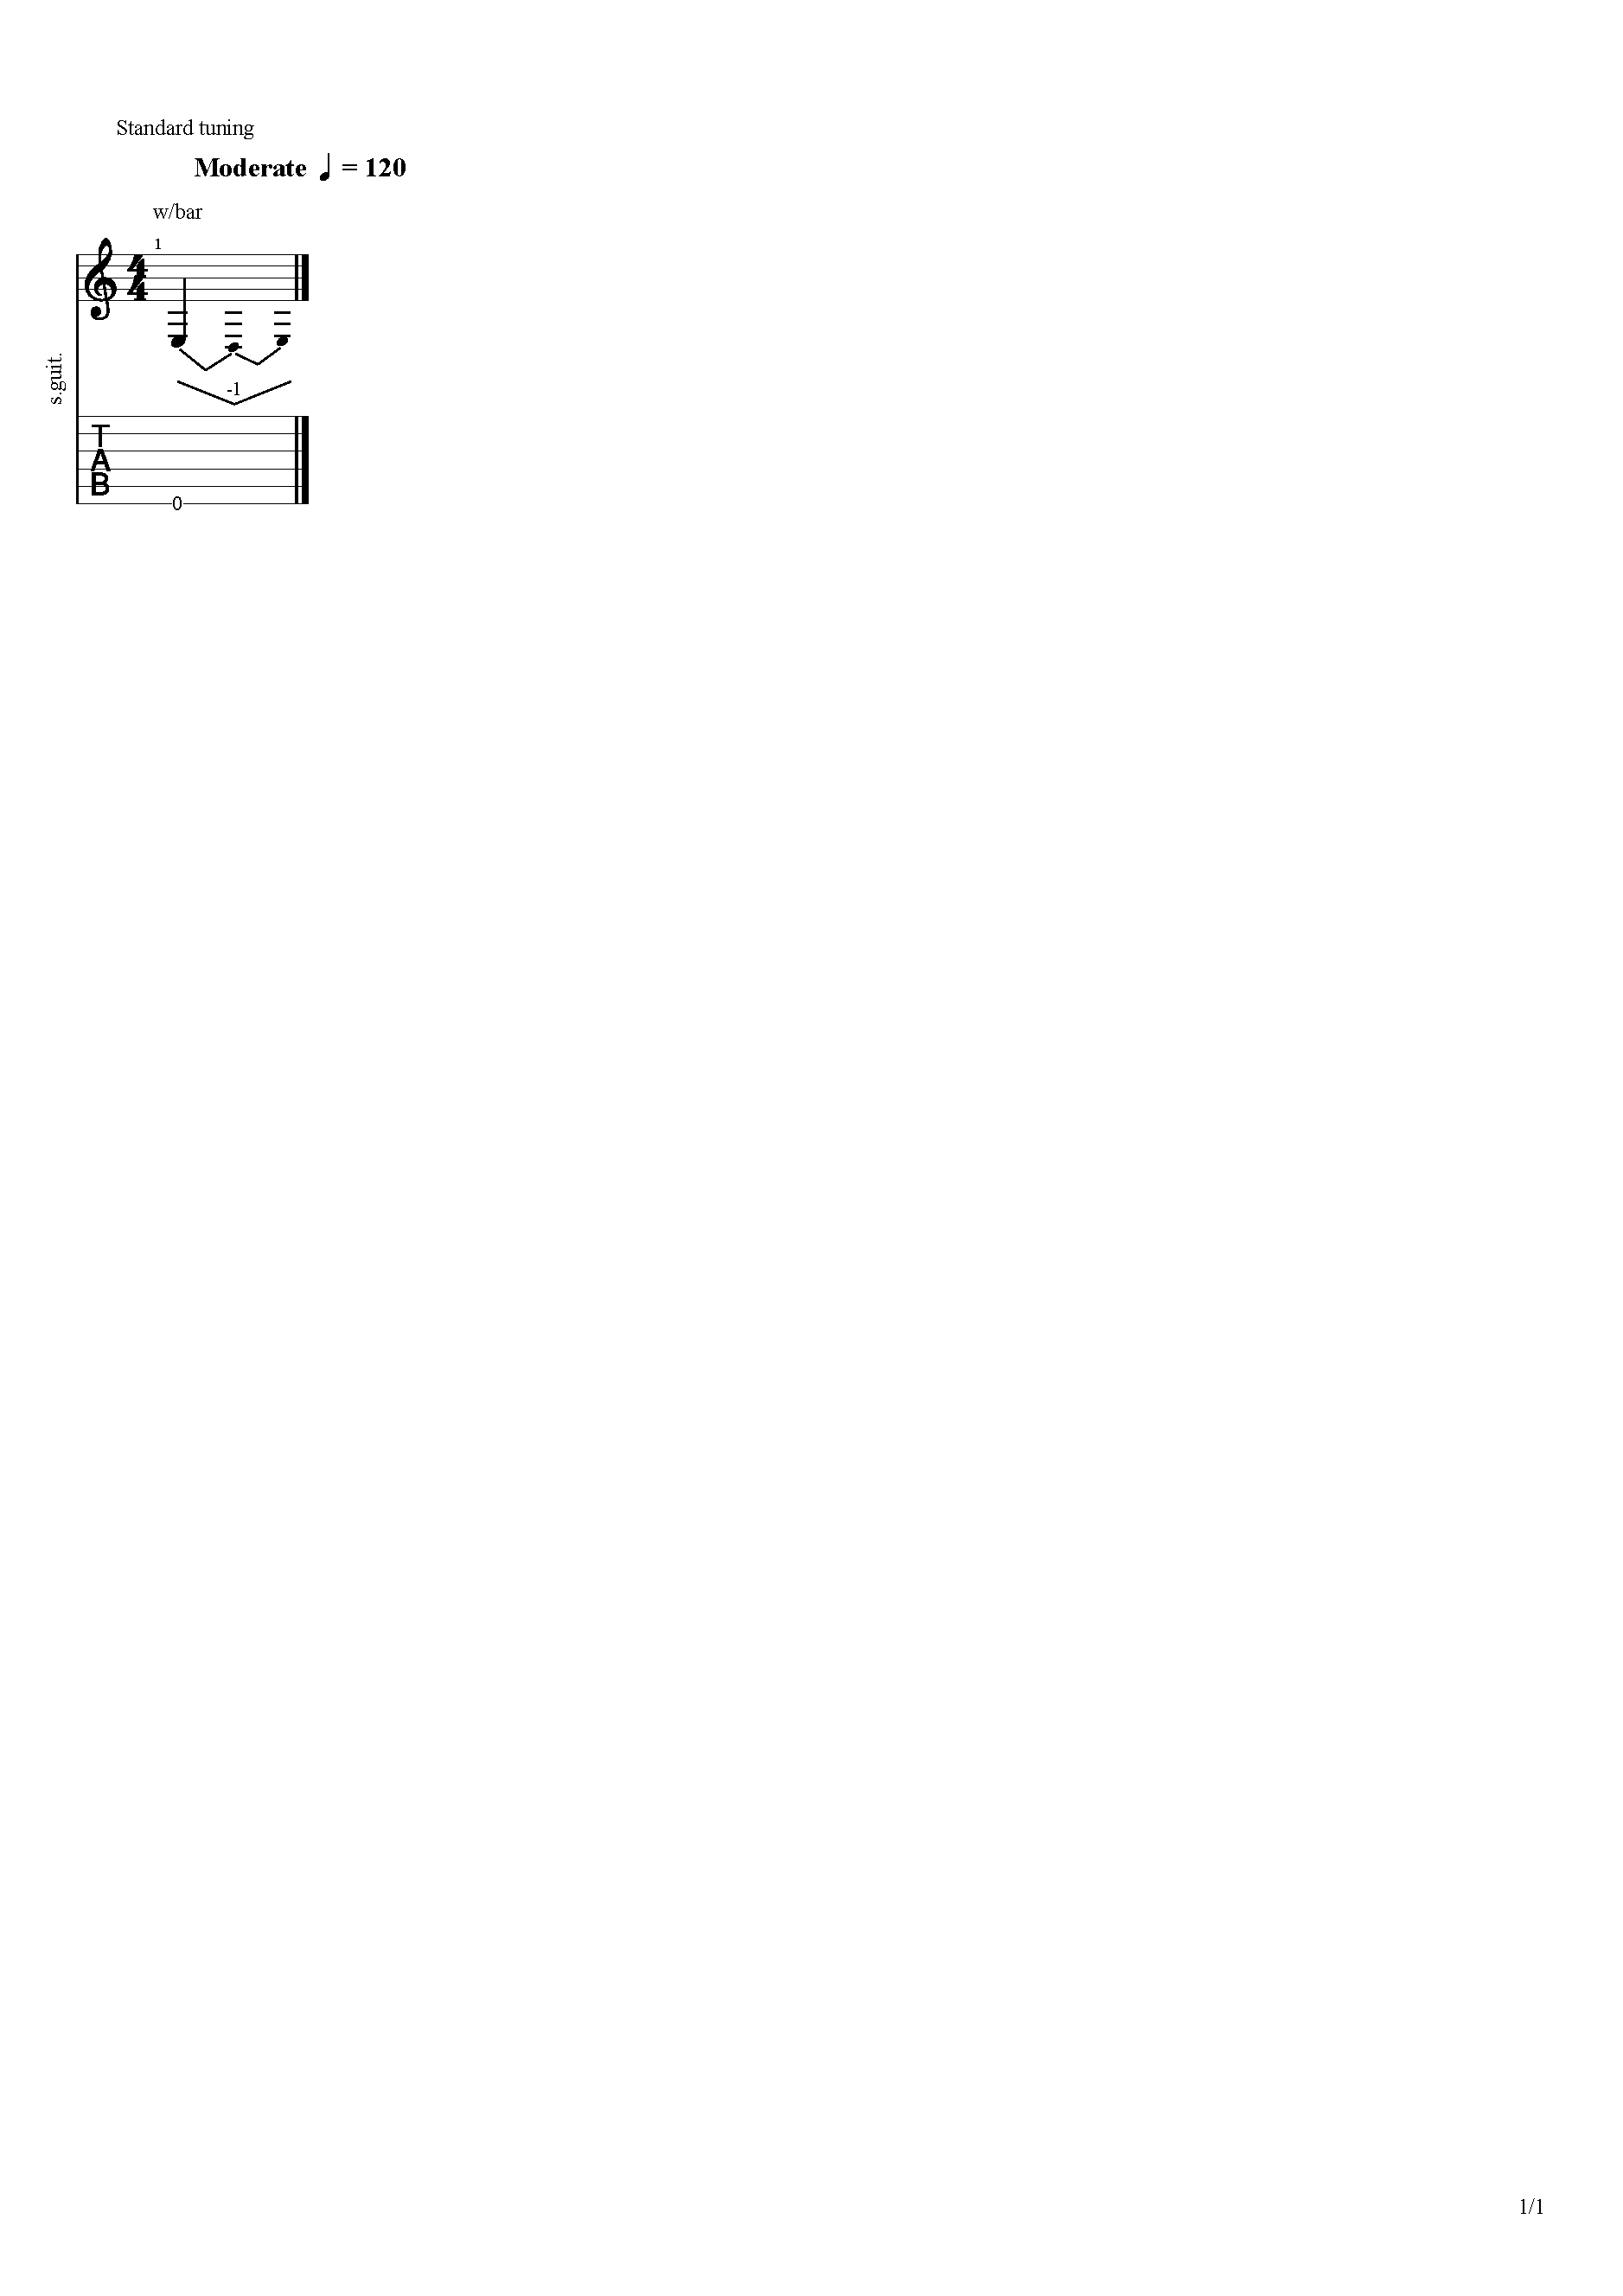
\includegraphics[trim={40 980 690 100}, clip, width=0.195\linewidth]{trem_2.pdf}
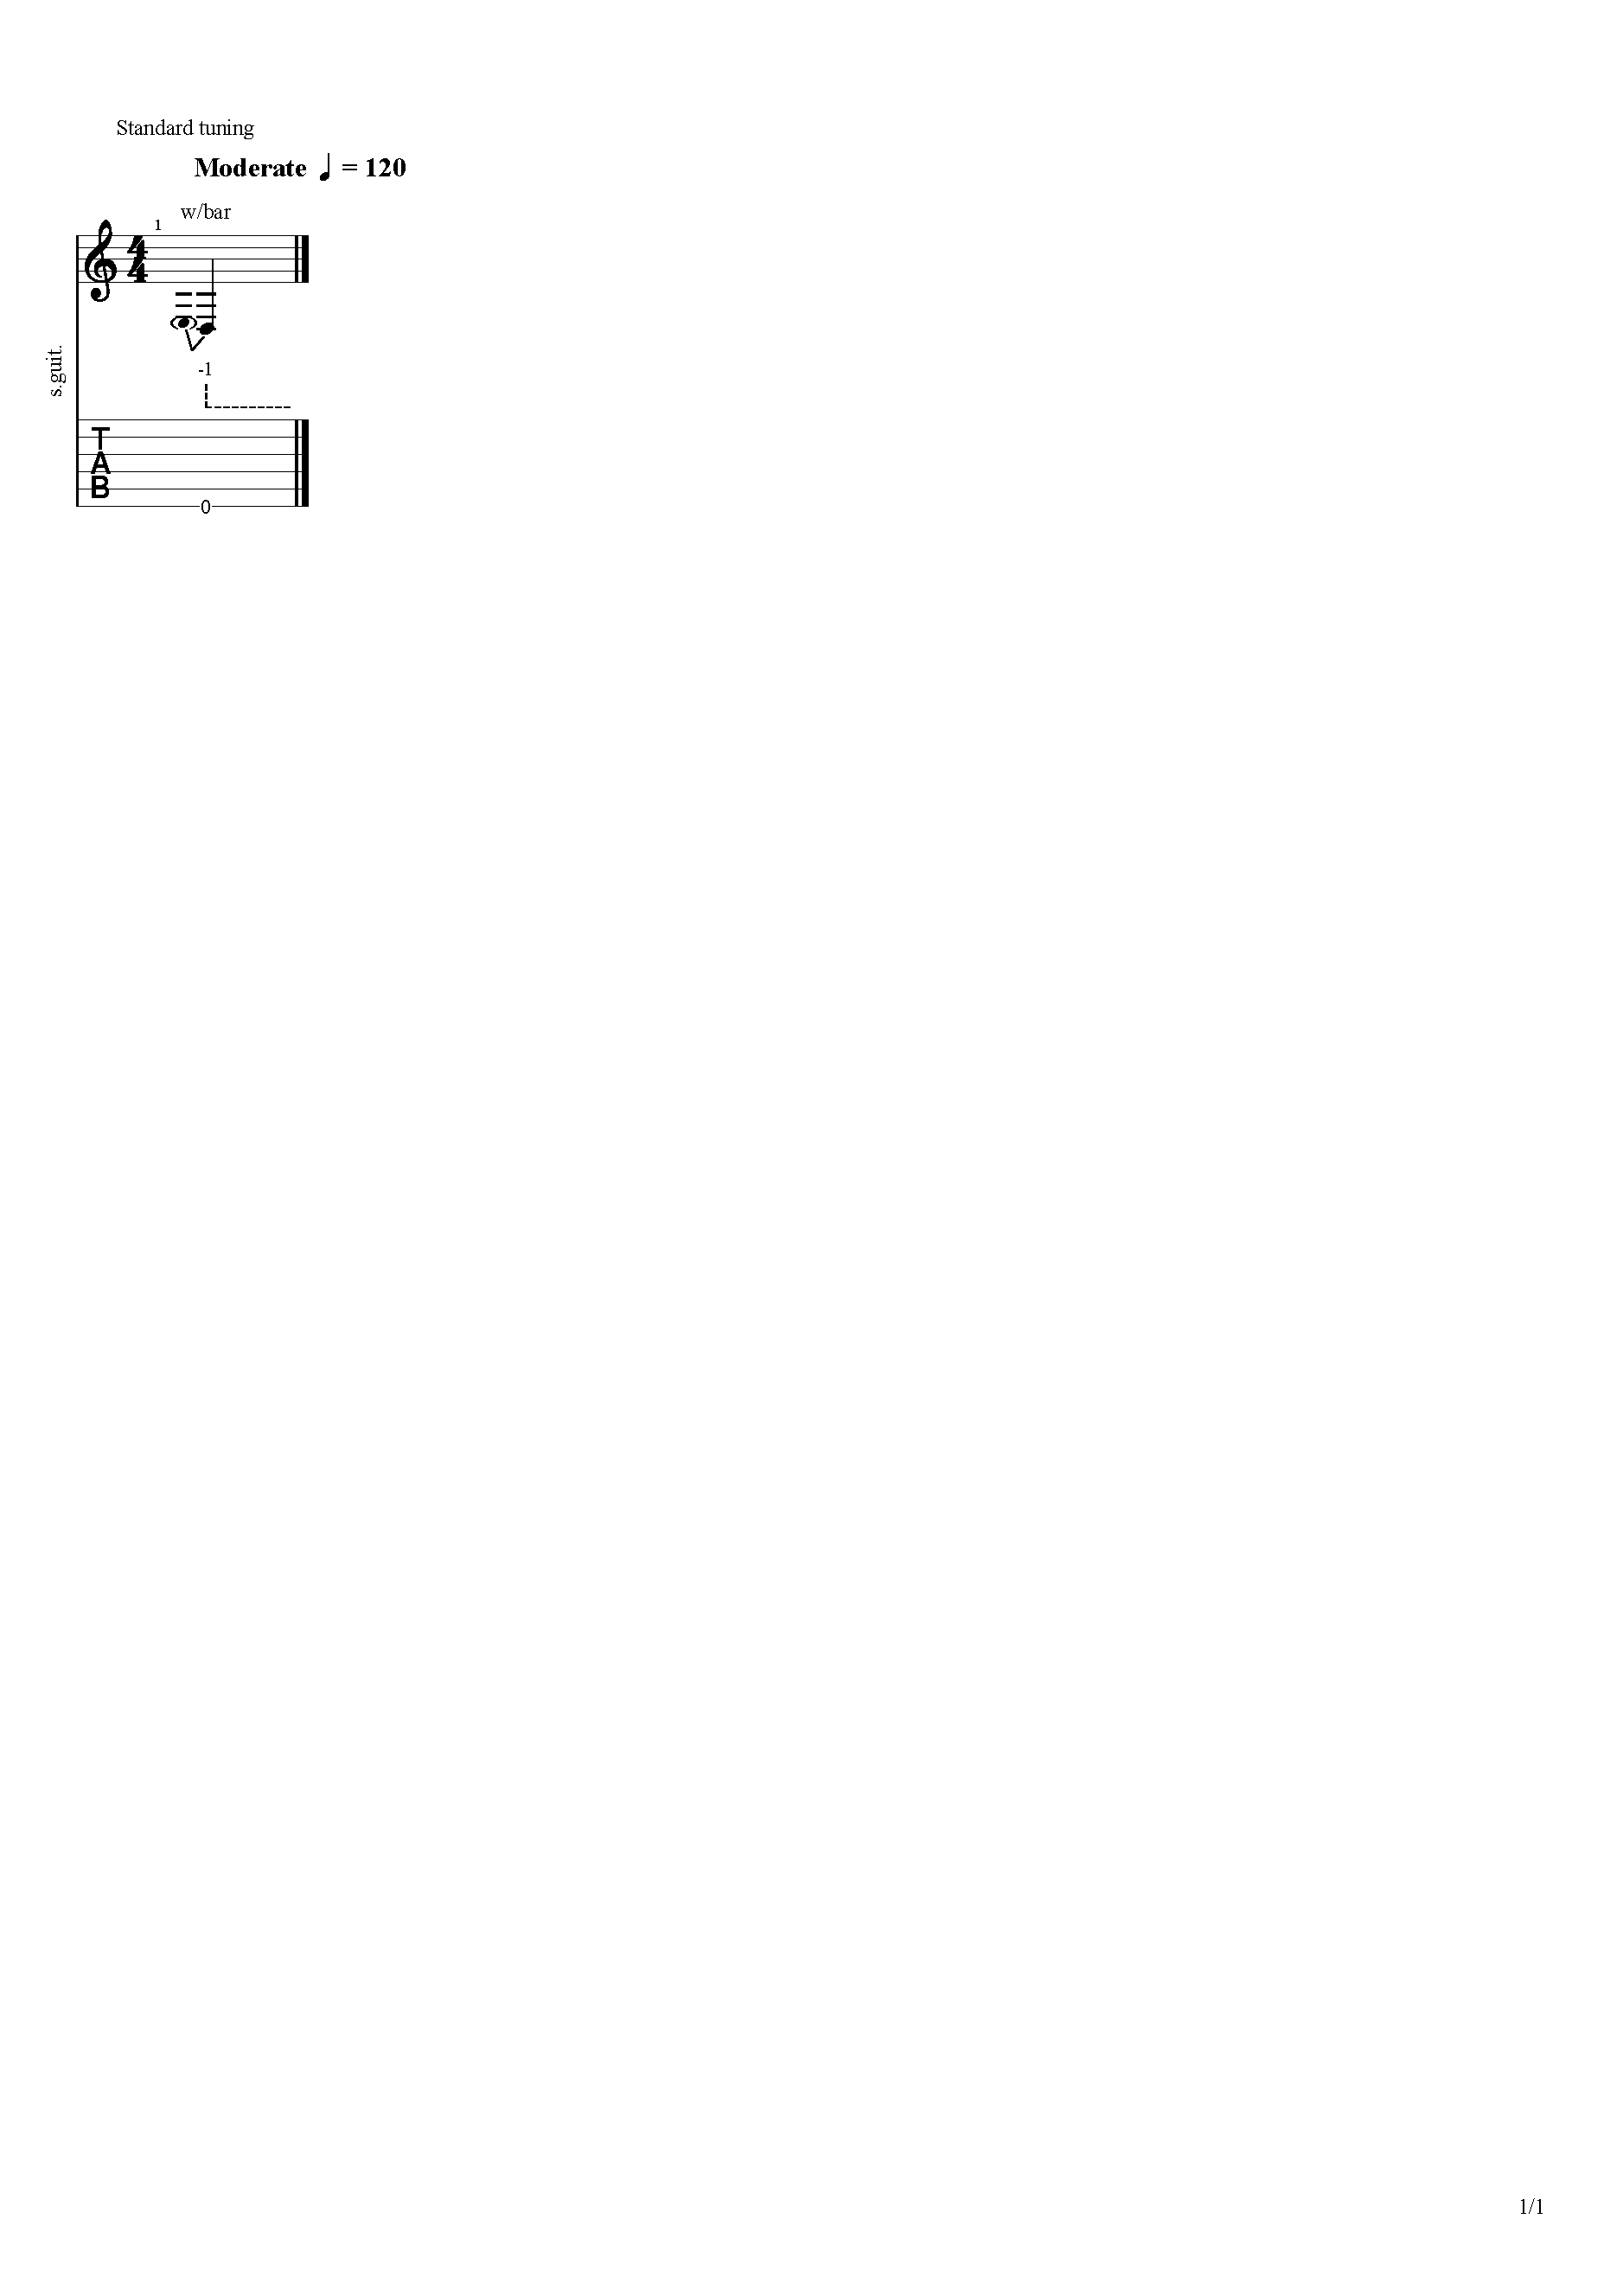
\includegraphics[trim={40 980 690 100}, clip, width=0.195\linewidth]{trem_4.pdf}
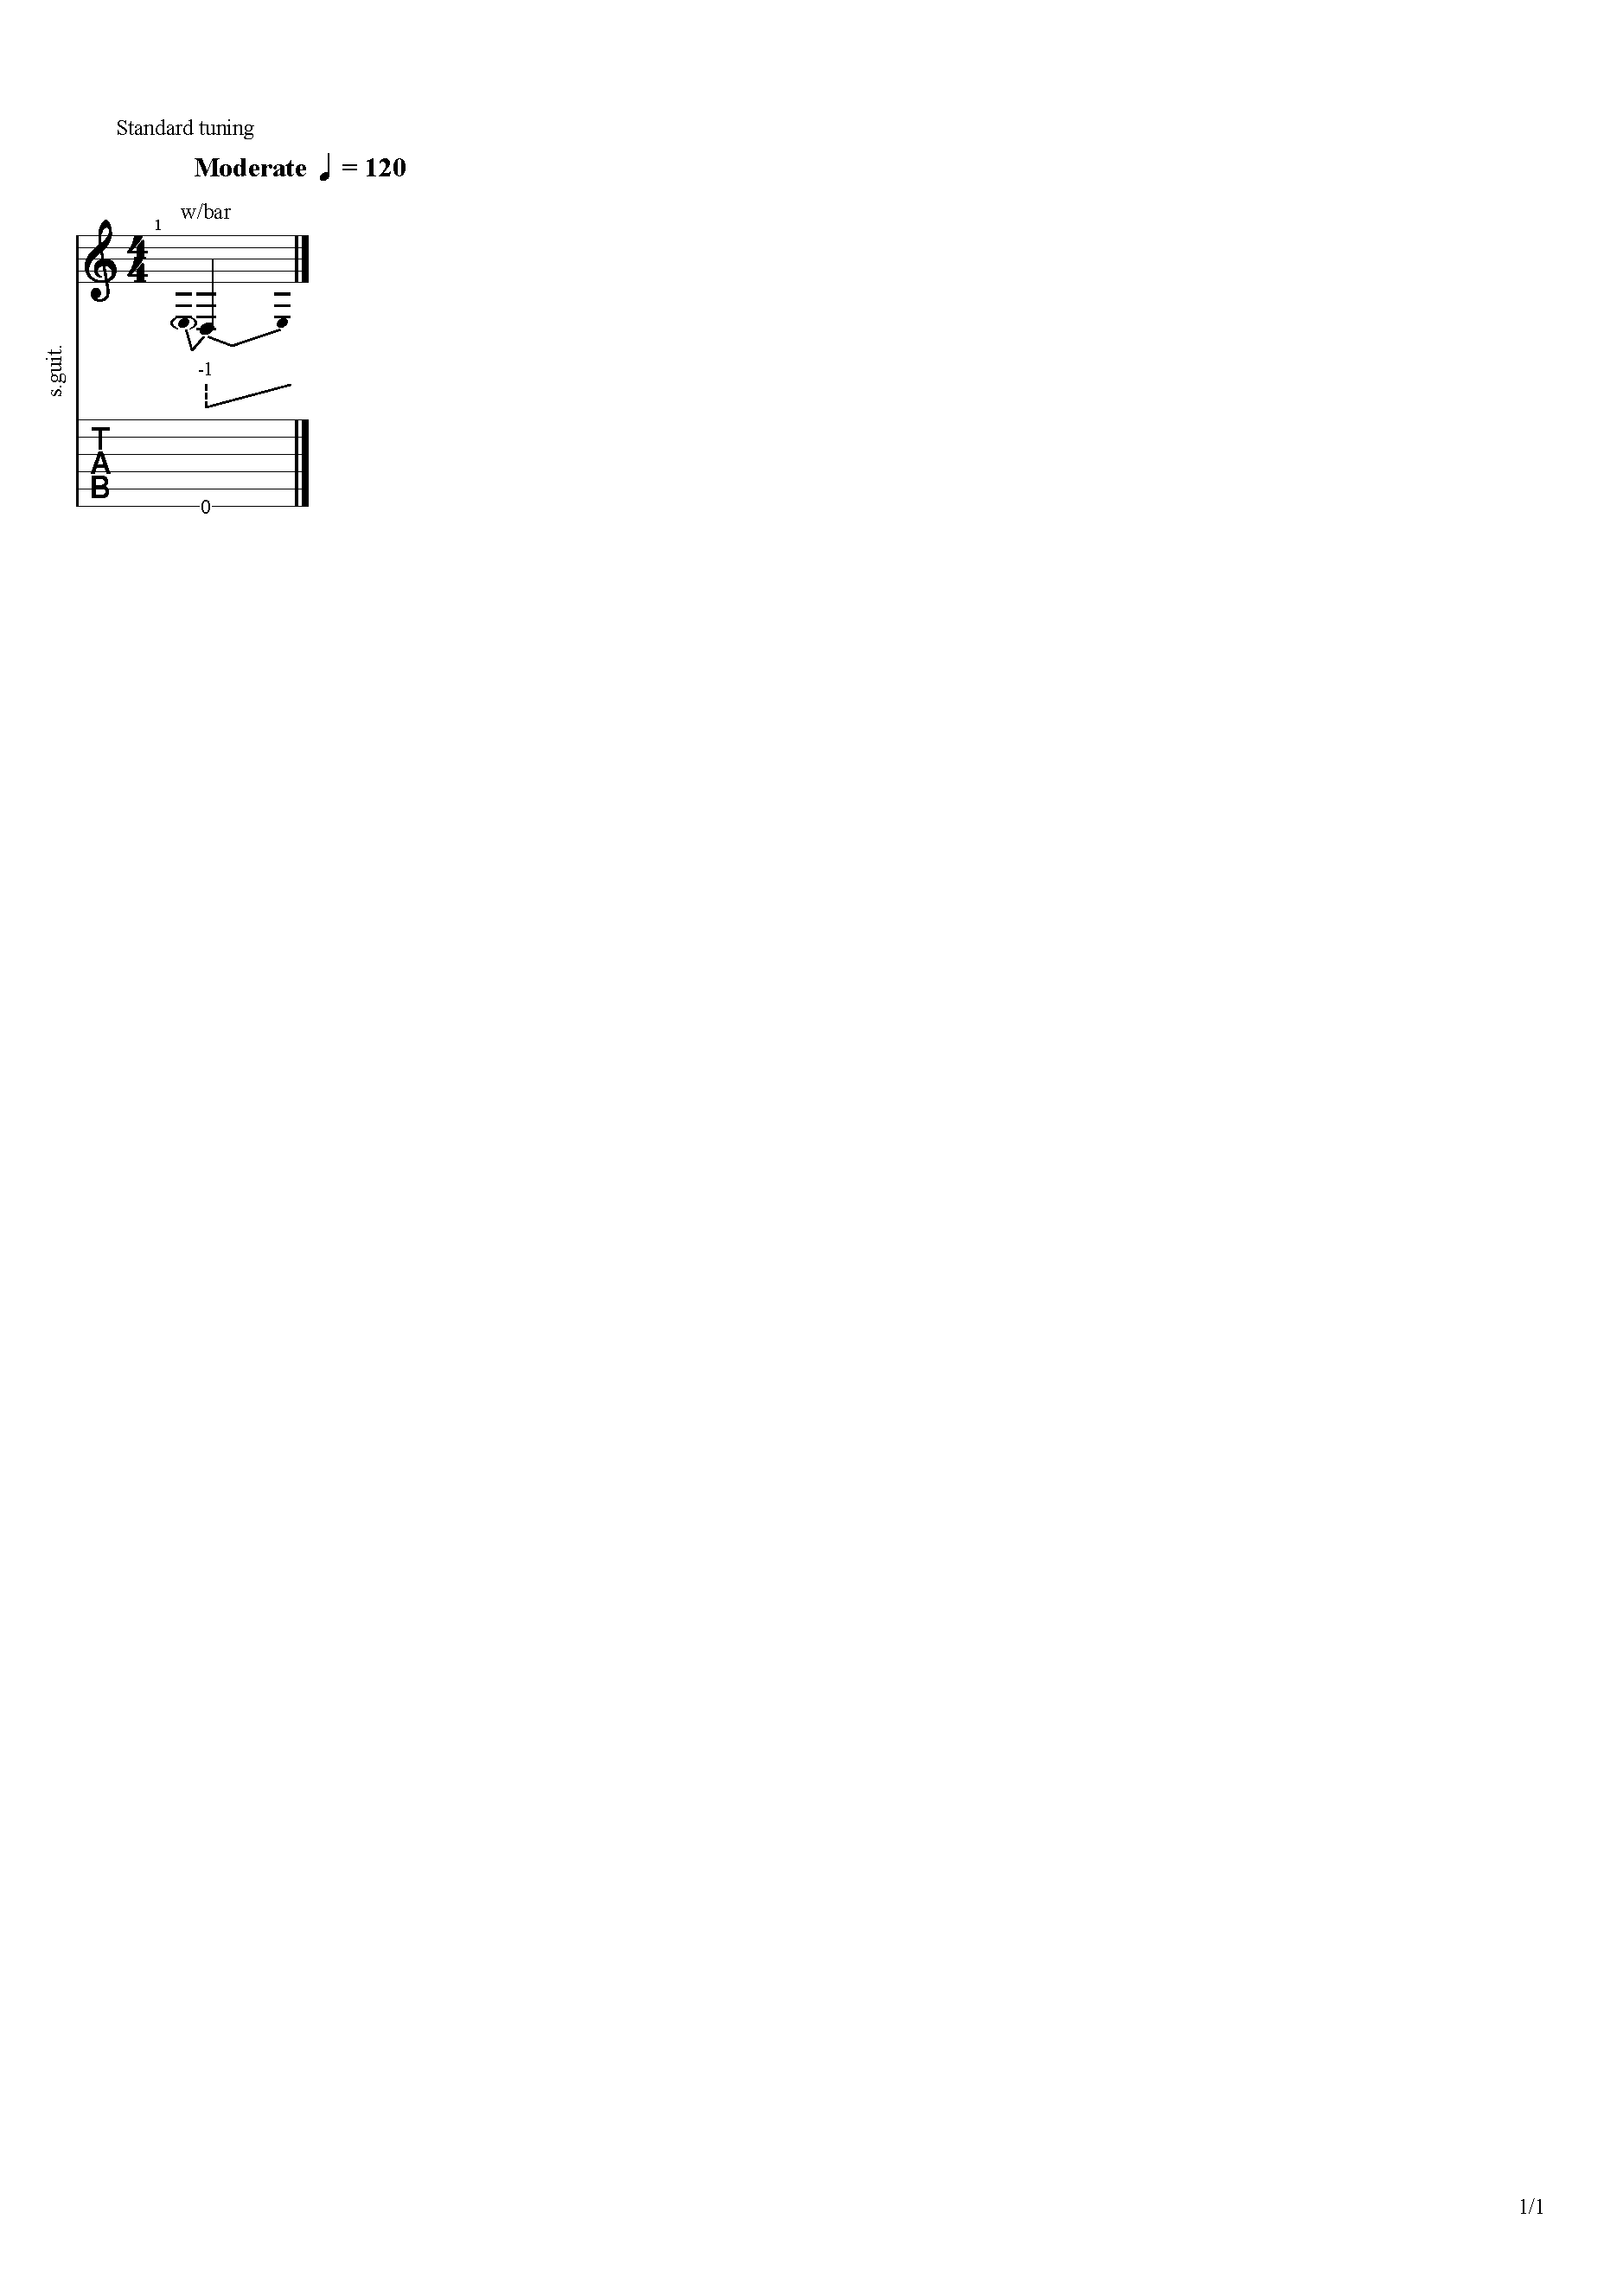
\includegraphics[trim={40 980 690 100}, clip, width=0.195\linewidth]{trem_5.pdf}
\caption{Tremlo types and their pitch variations.}
  \label{fig:trem}
\end{figure}
\subsubsection{Slide}
Smoothly moving up or down the fretboard without lifting off on the string, creating a seamless transition between notes.
\begin{figure}[htbp]
  \centering
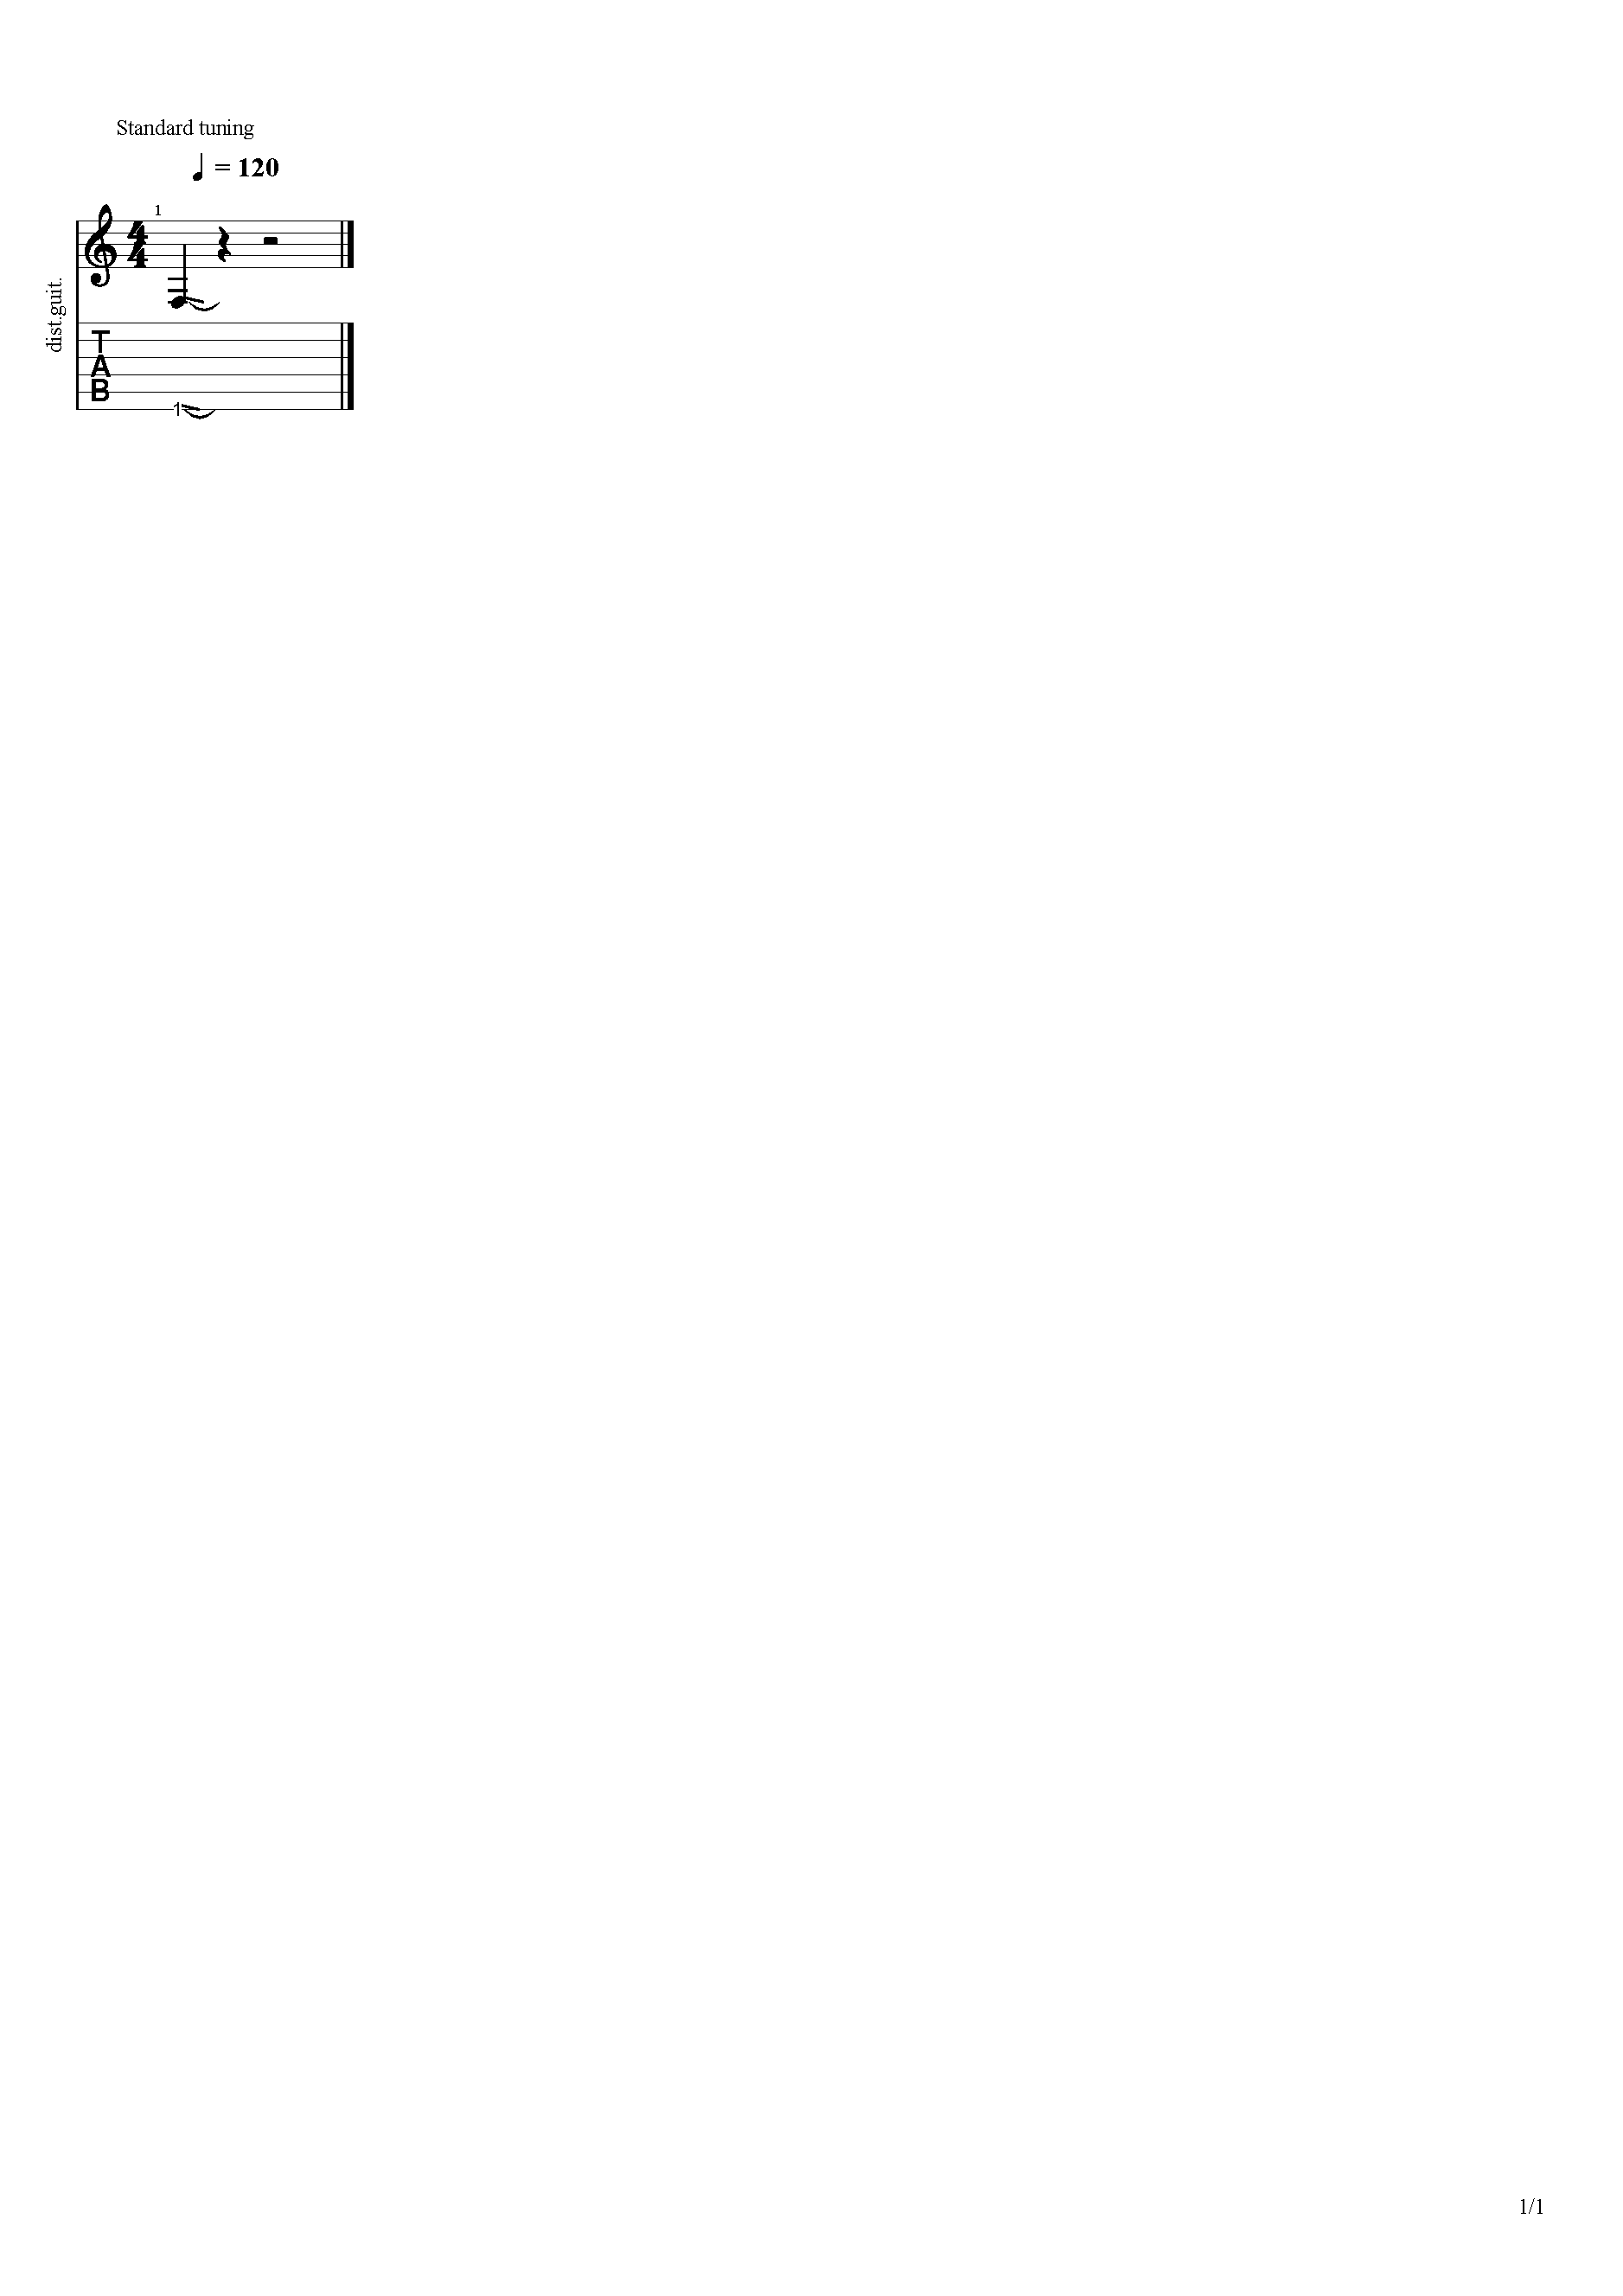
\includegraphics[trim={40 1040 690 100}, clip, width=0.16\linewidth]{slide_1.pdf}
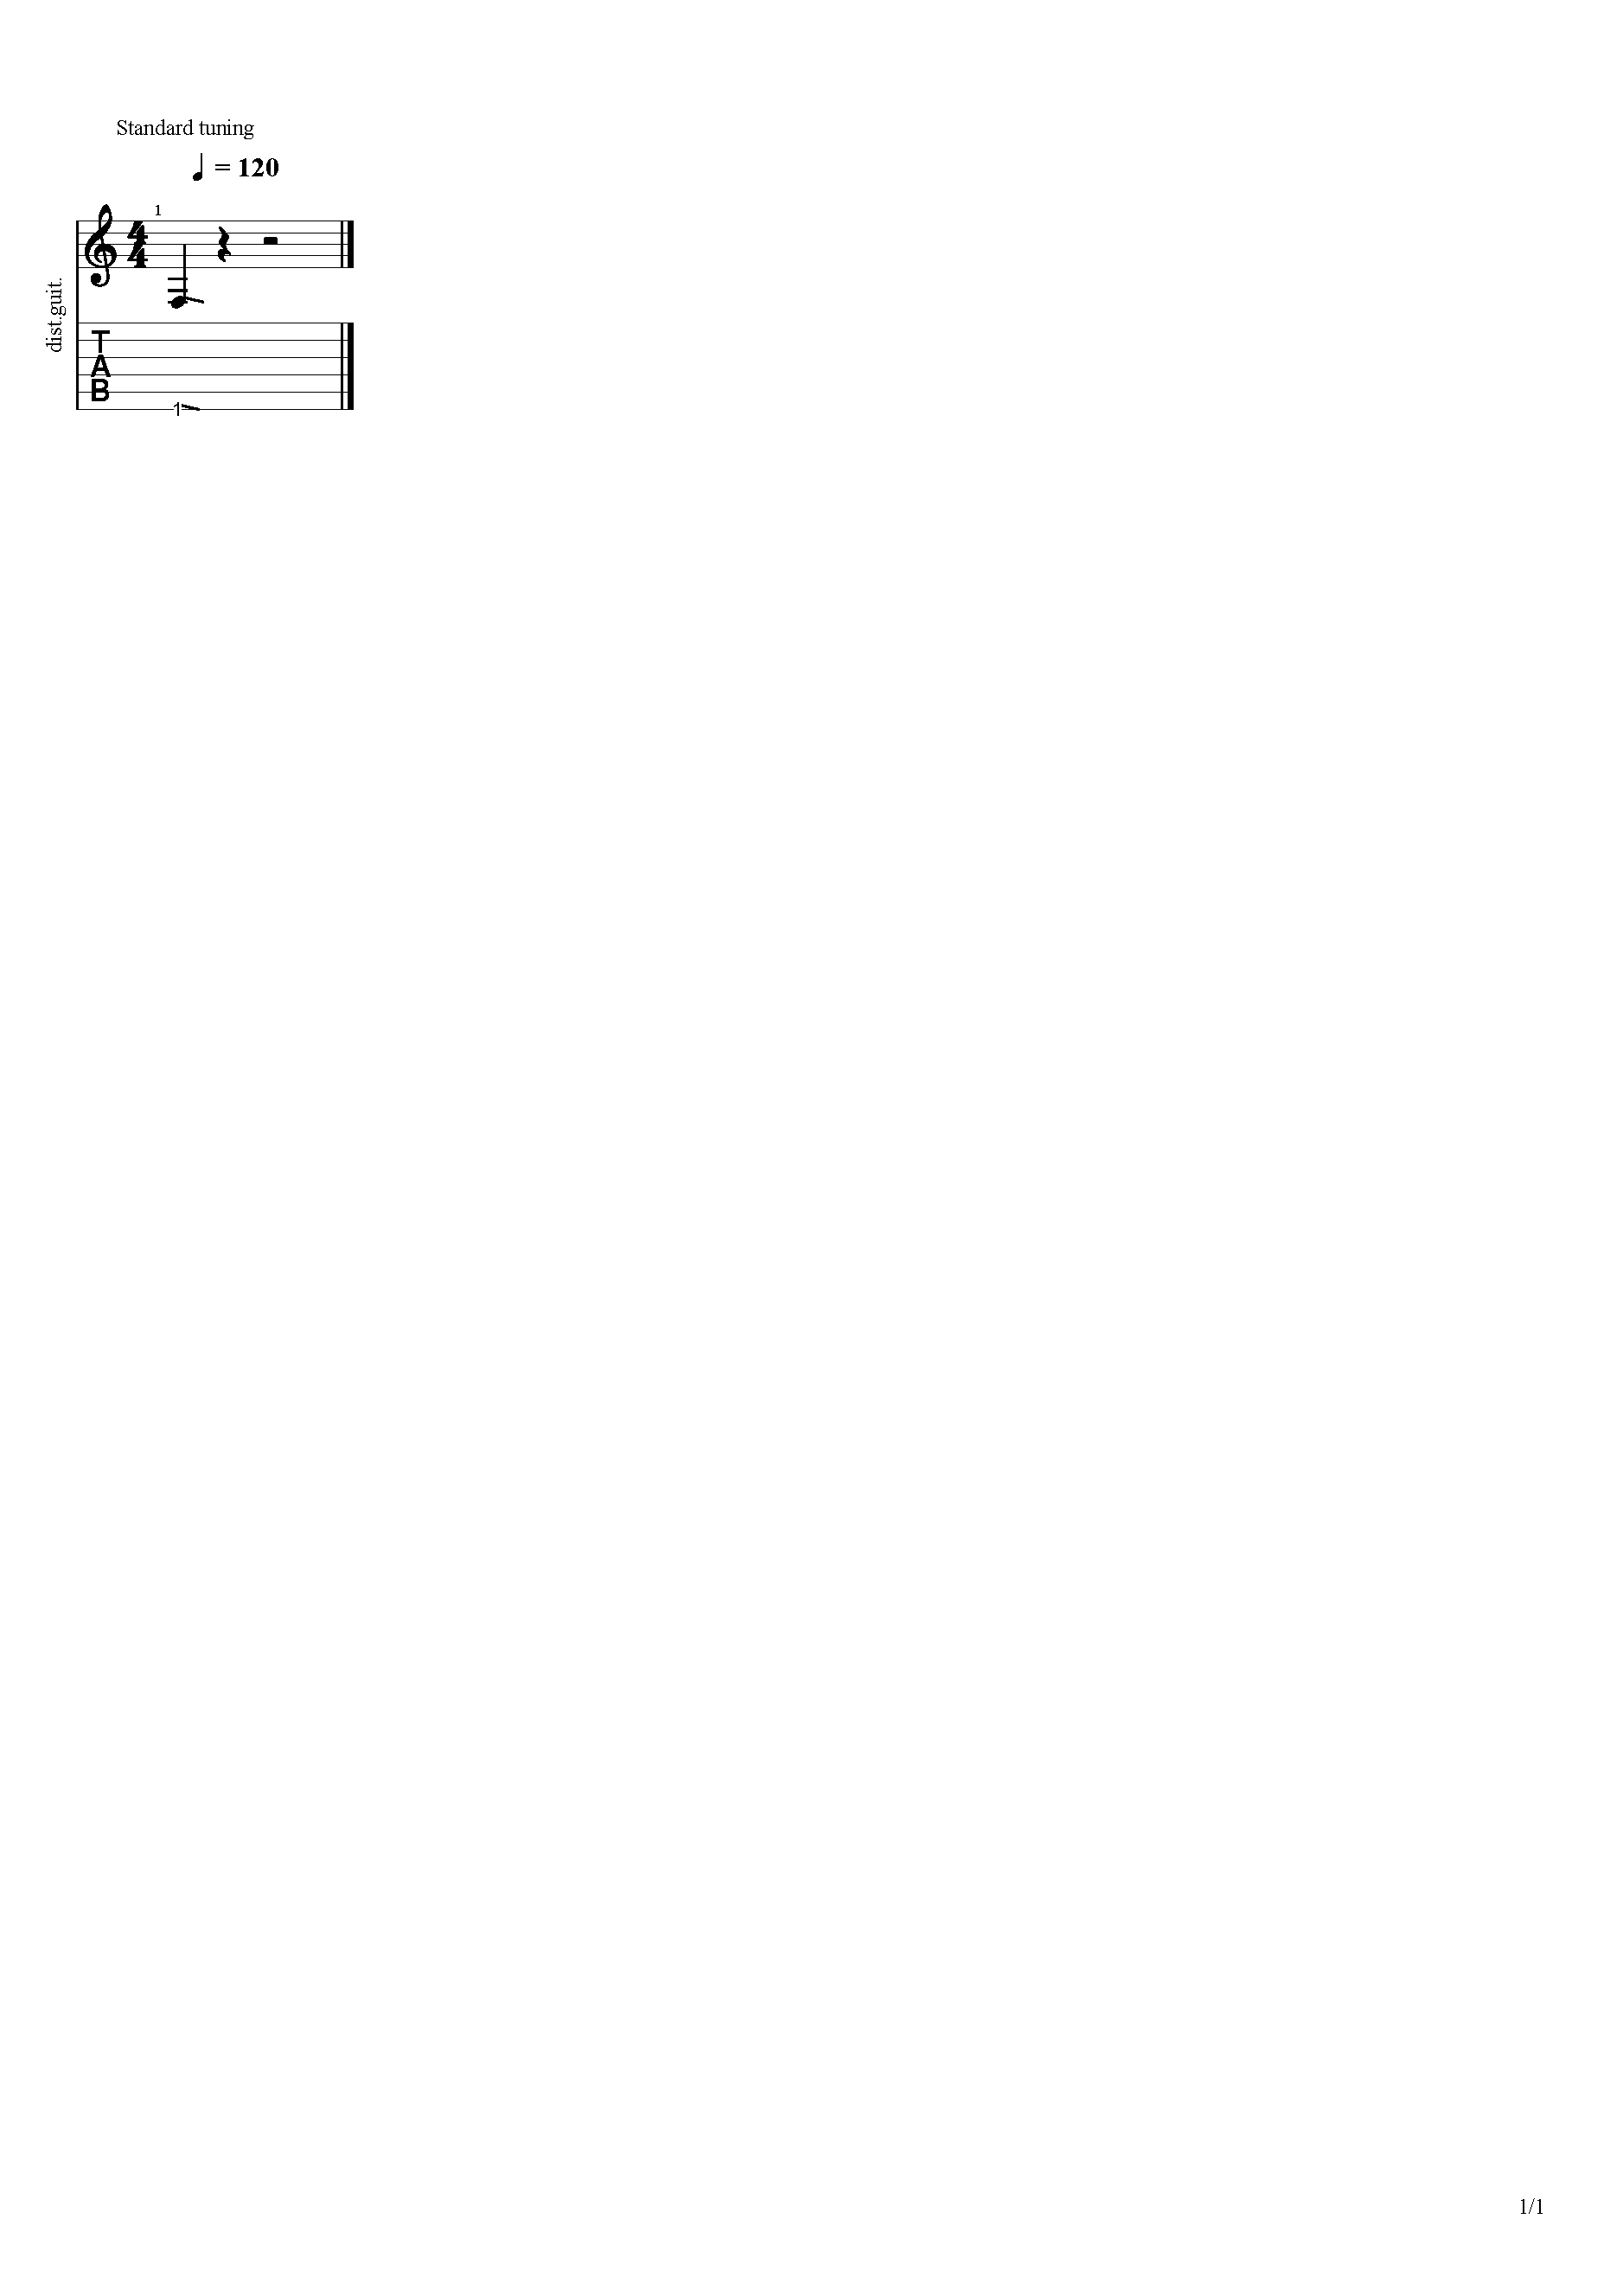
\includegraphics[trim={40 1040 690 100}, clip, width=0.16\linewidth]{slide_2.pdf}
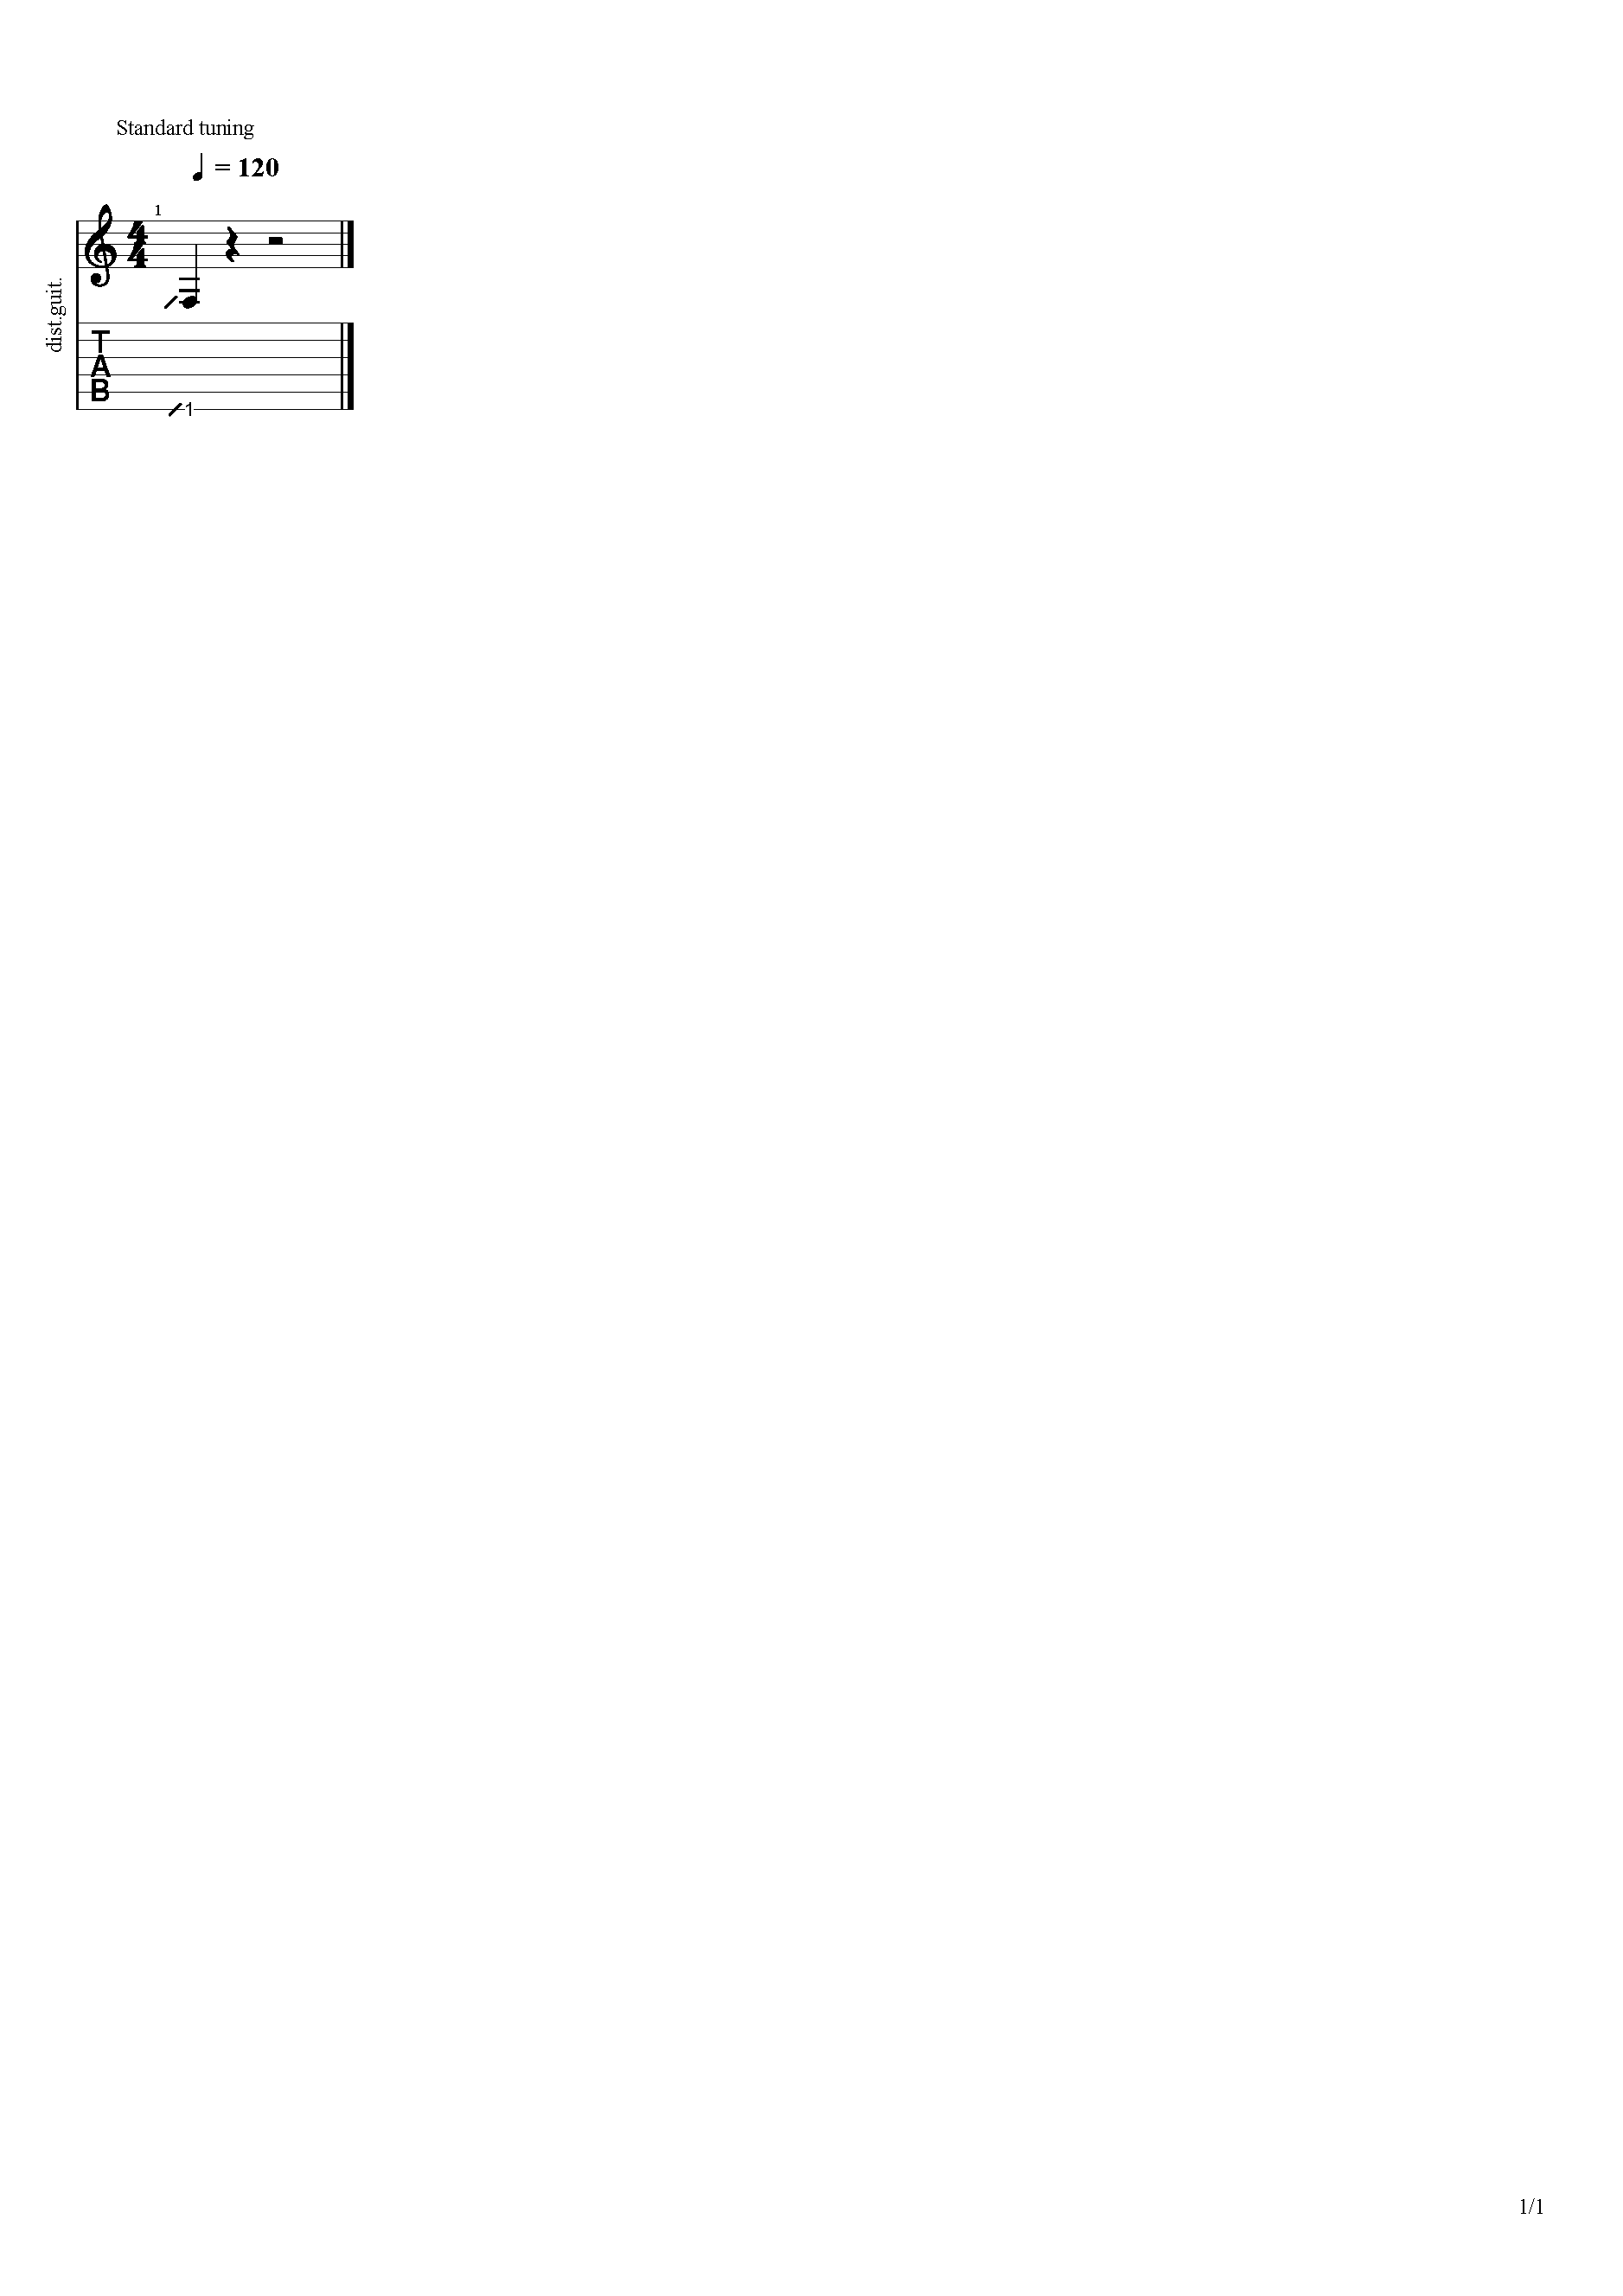
\includegraphics[trim={40 1040 690 100}, clip, width=0.16\linewidth]{slide_3.pdf}
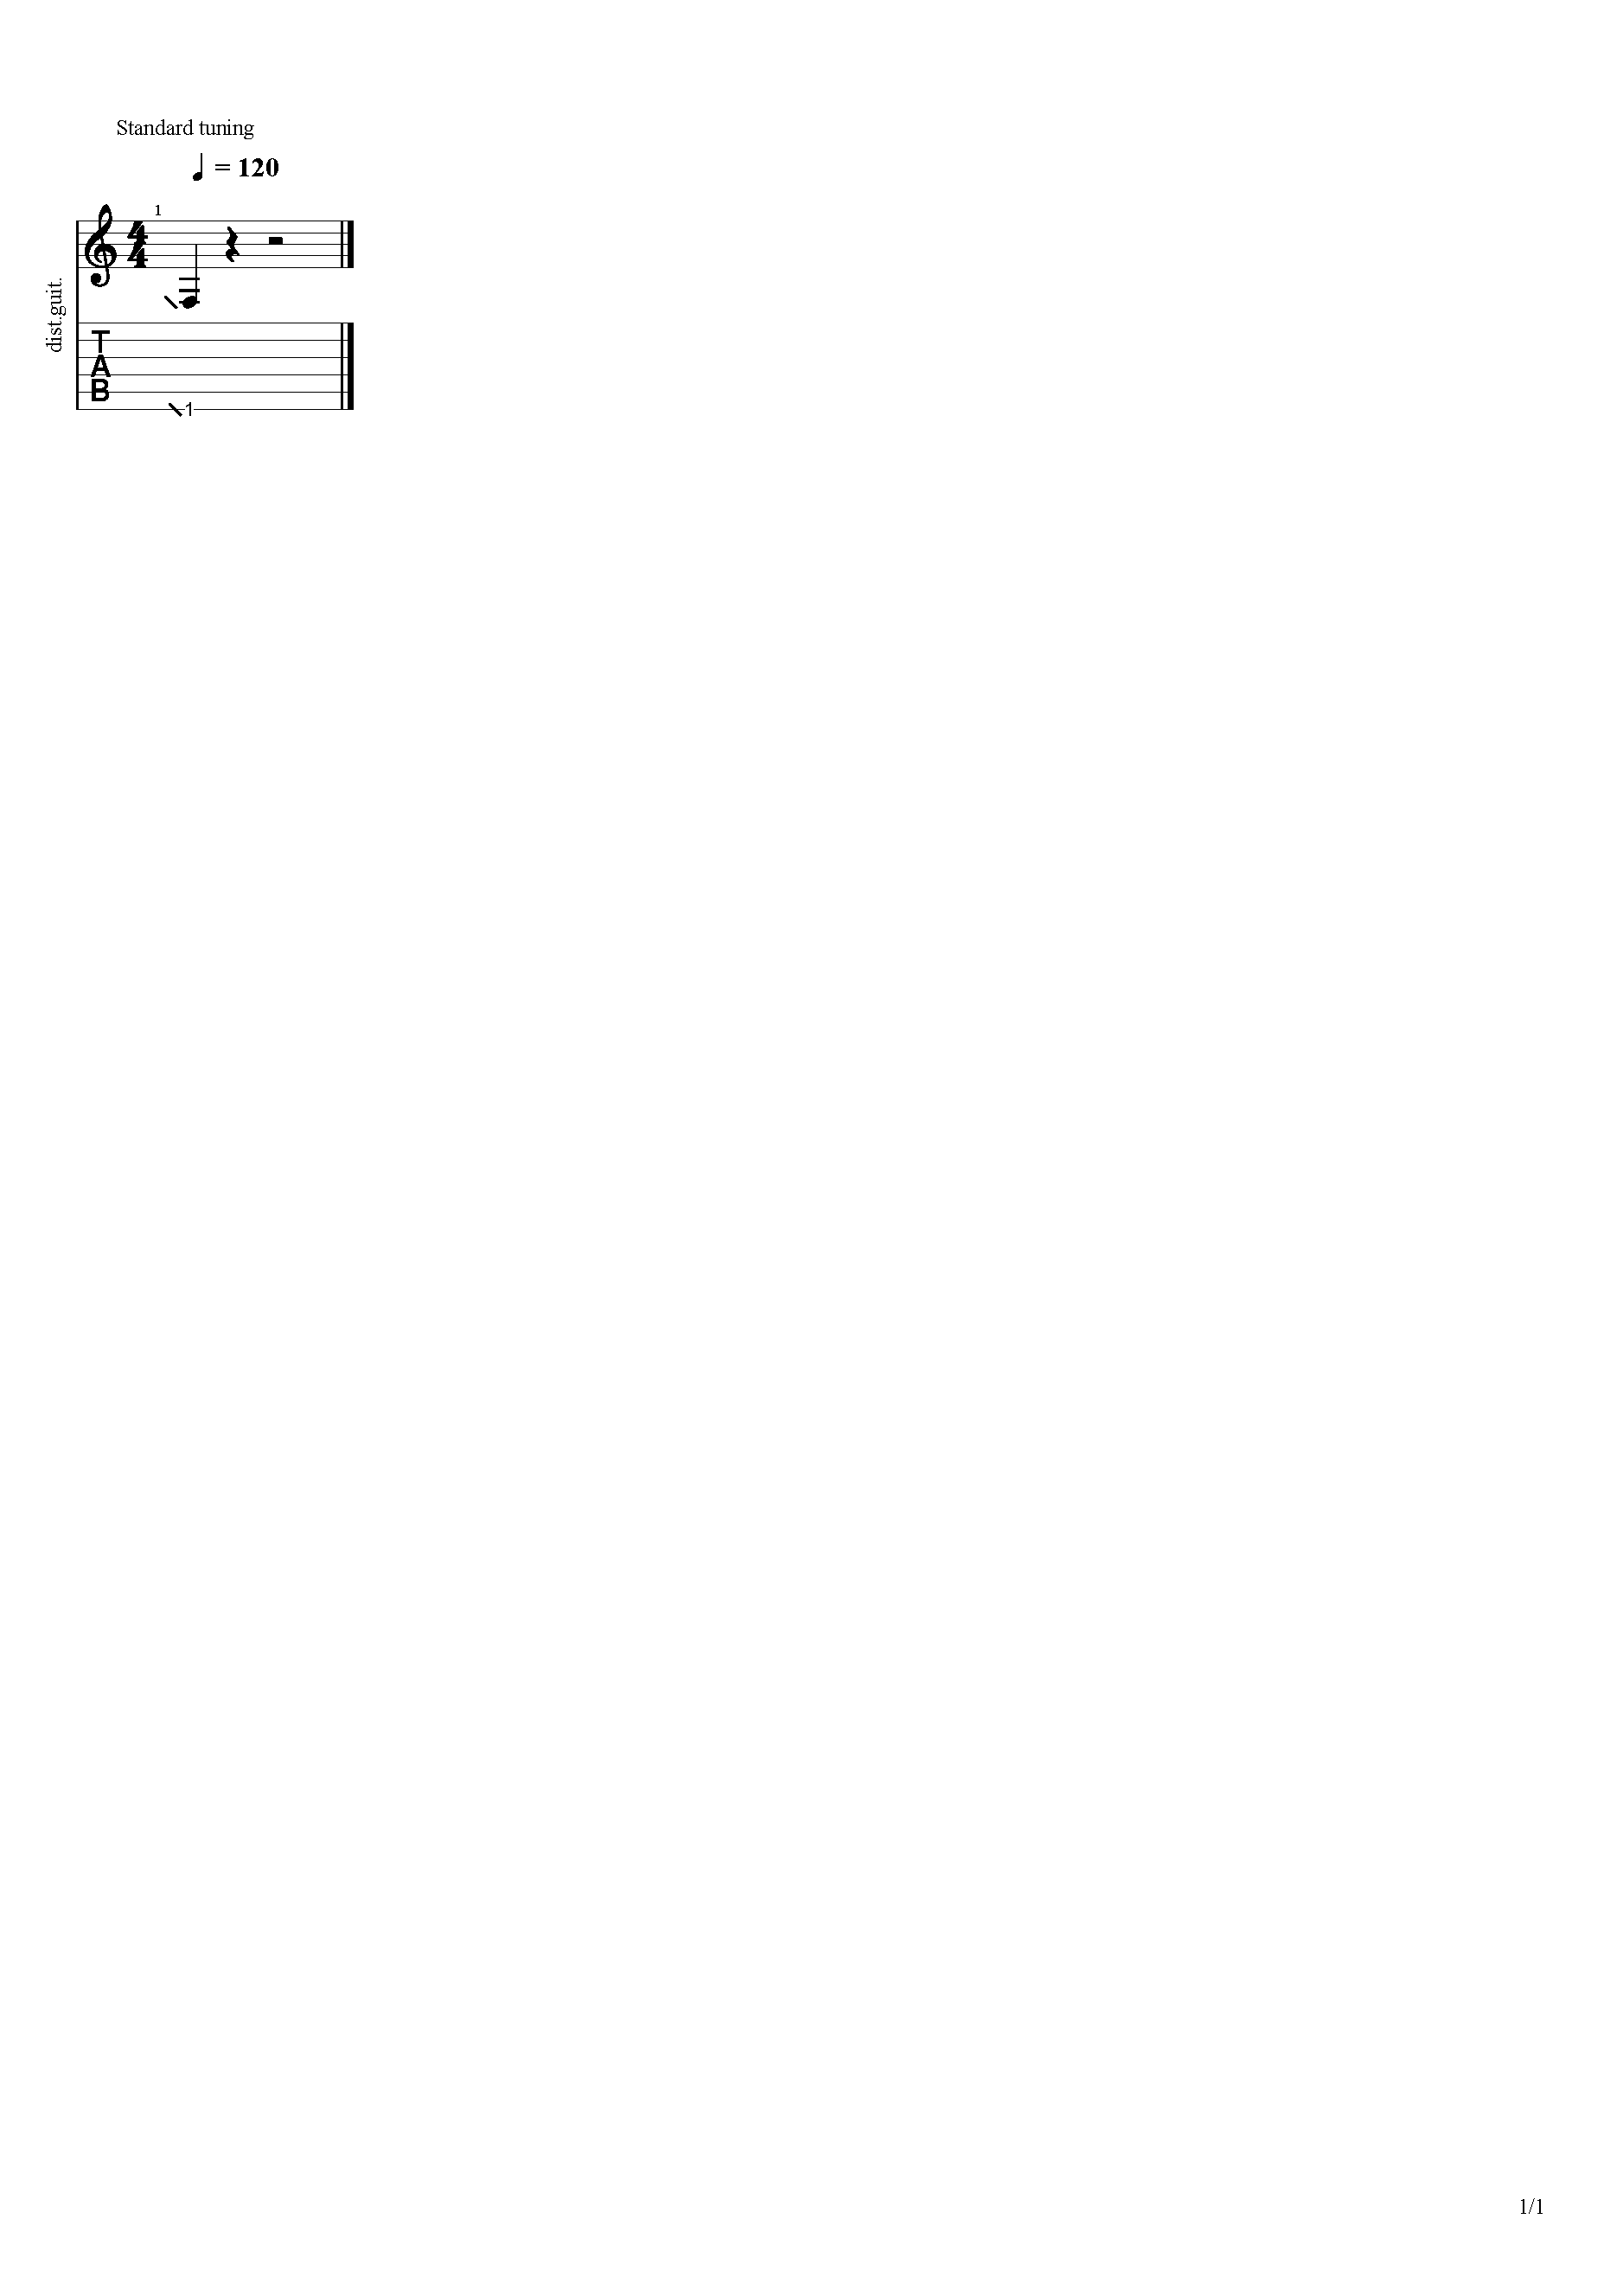
\includegraphics[trim={40 1040 690 100}, clip, width=0.16\linewidth]{slide_4.pdf}
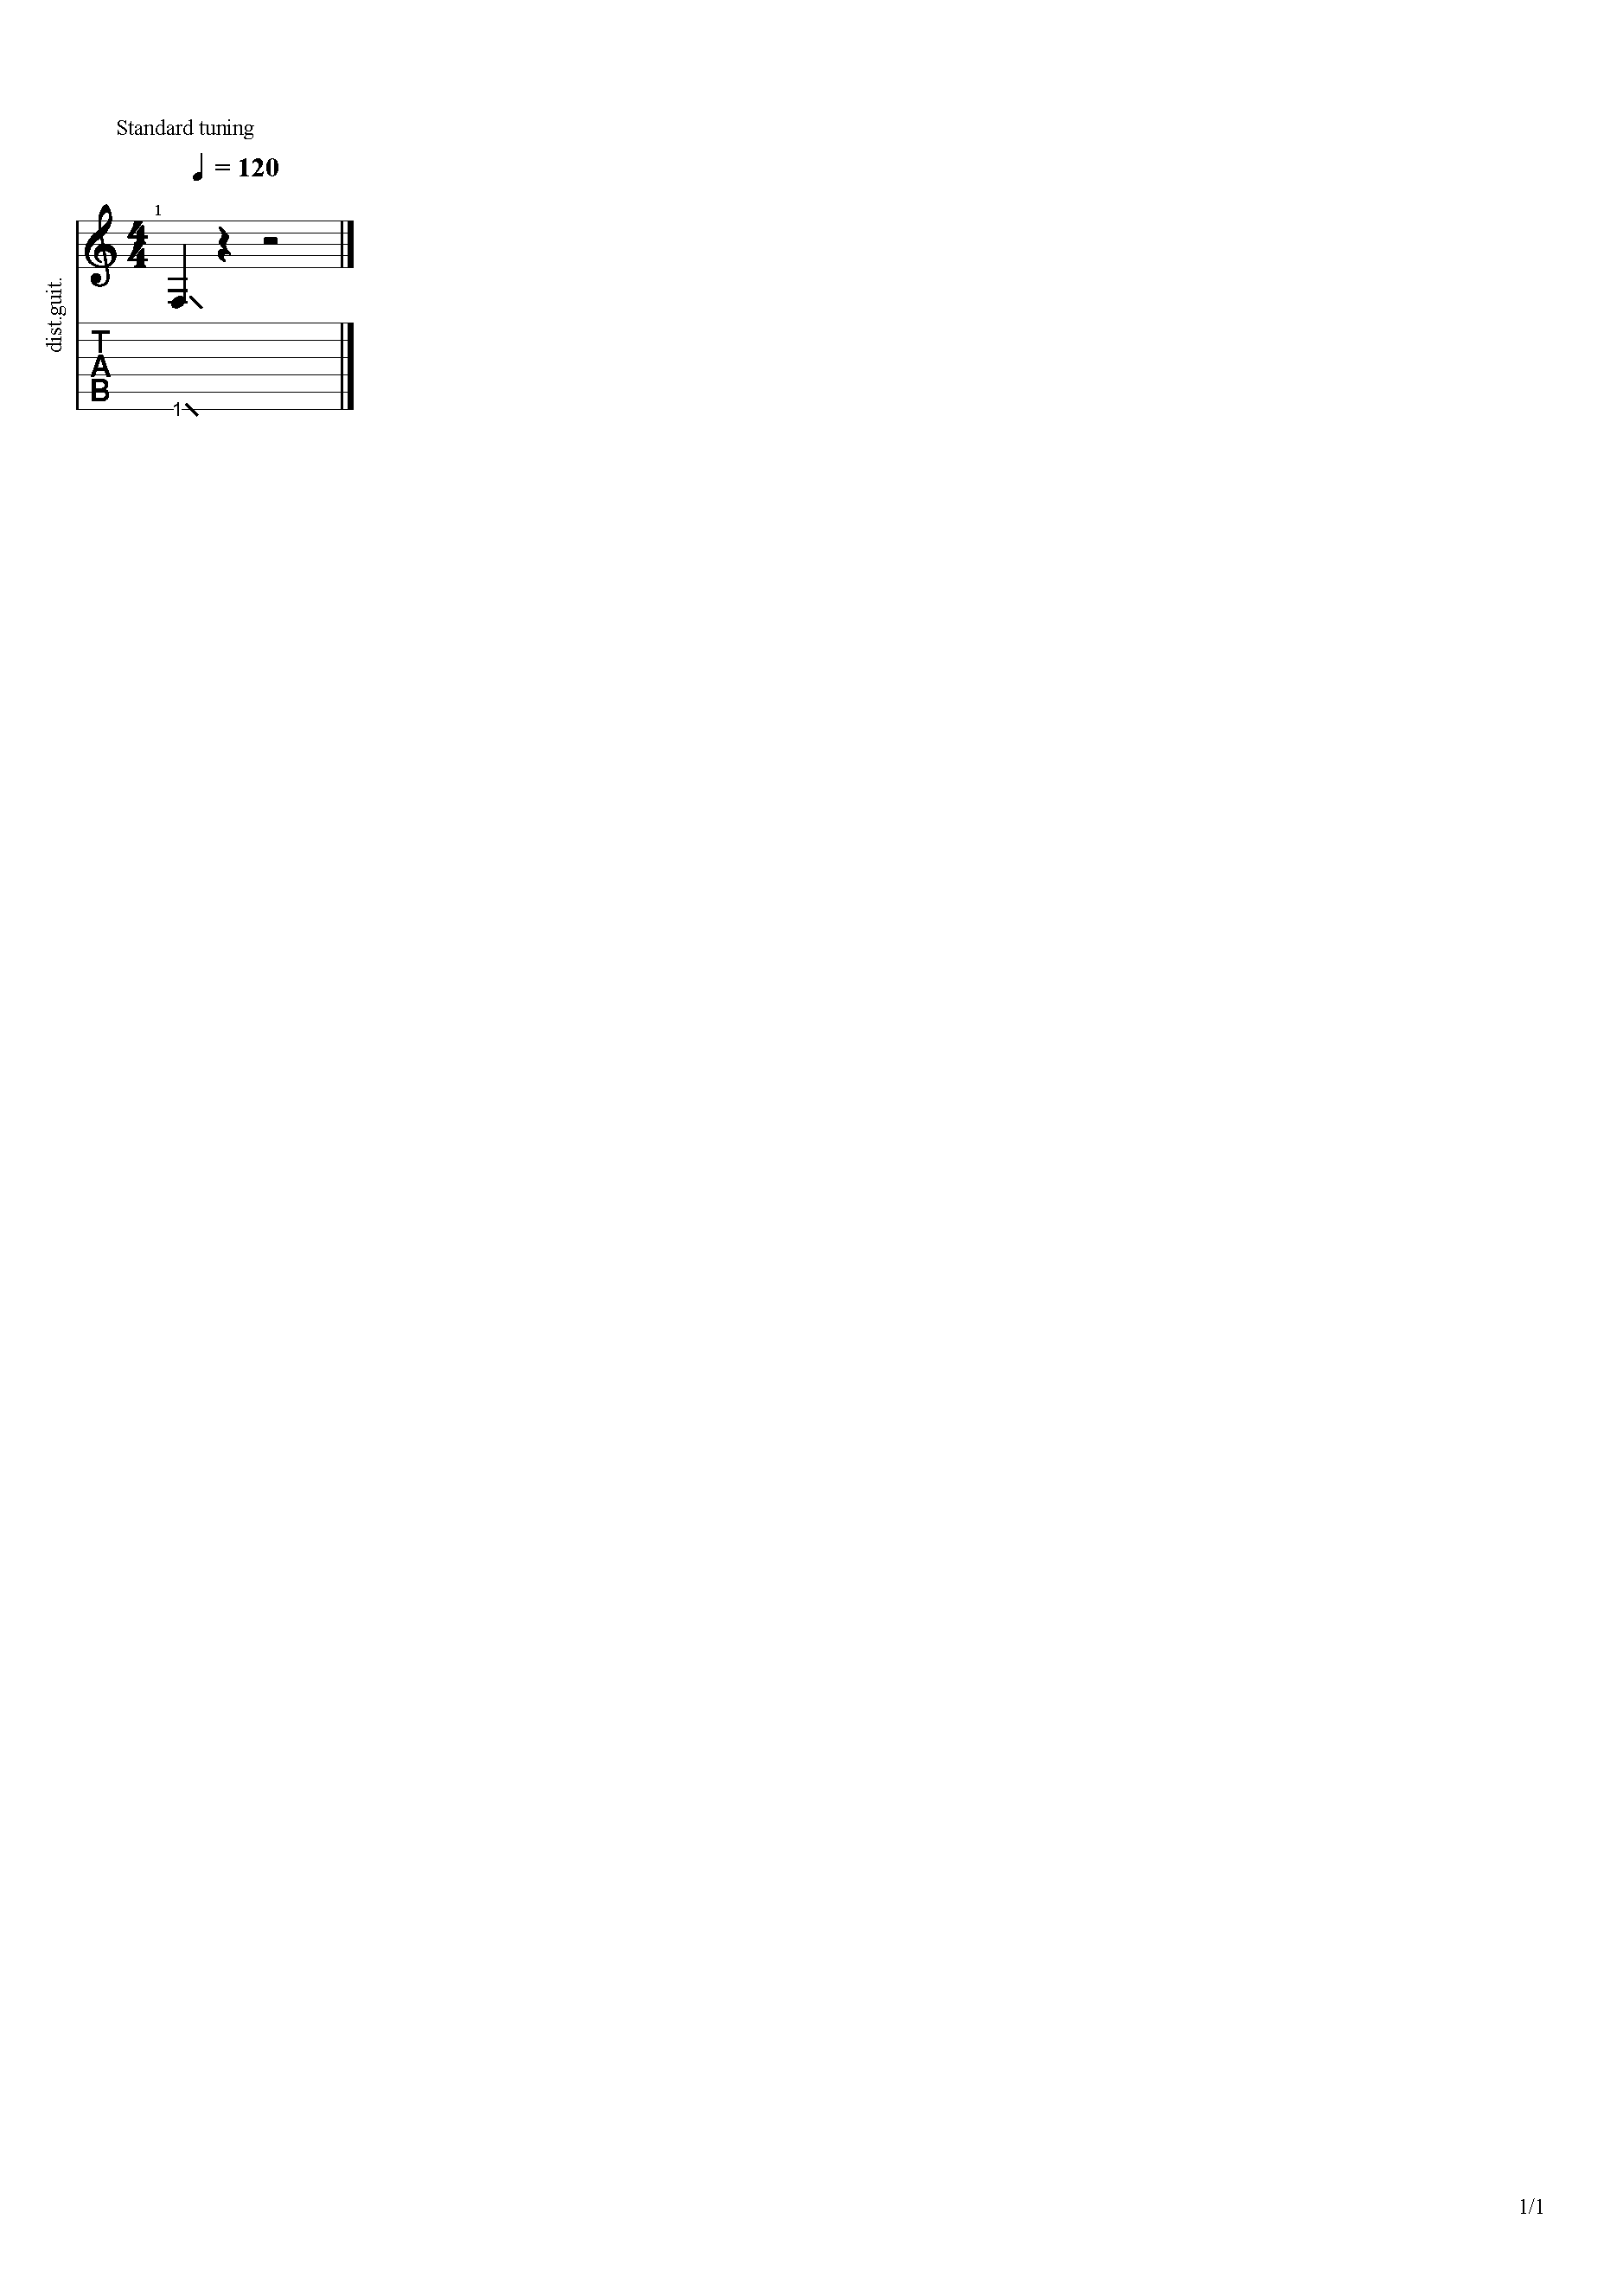
\includegraphics[trim={40 1040 690 100}, clip, width=0.16\linewidth]{slide_5.pdf}
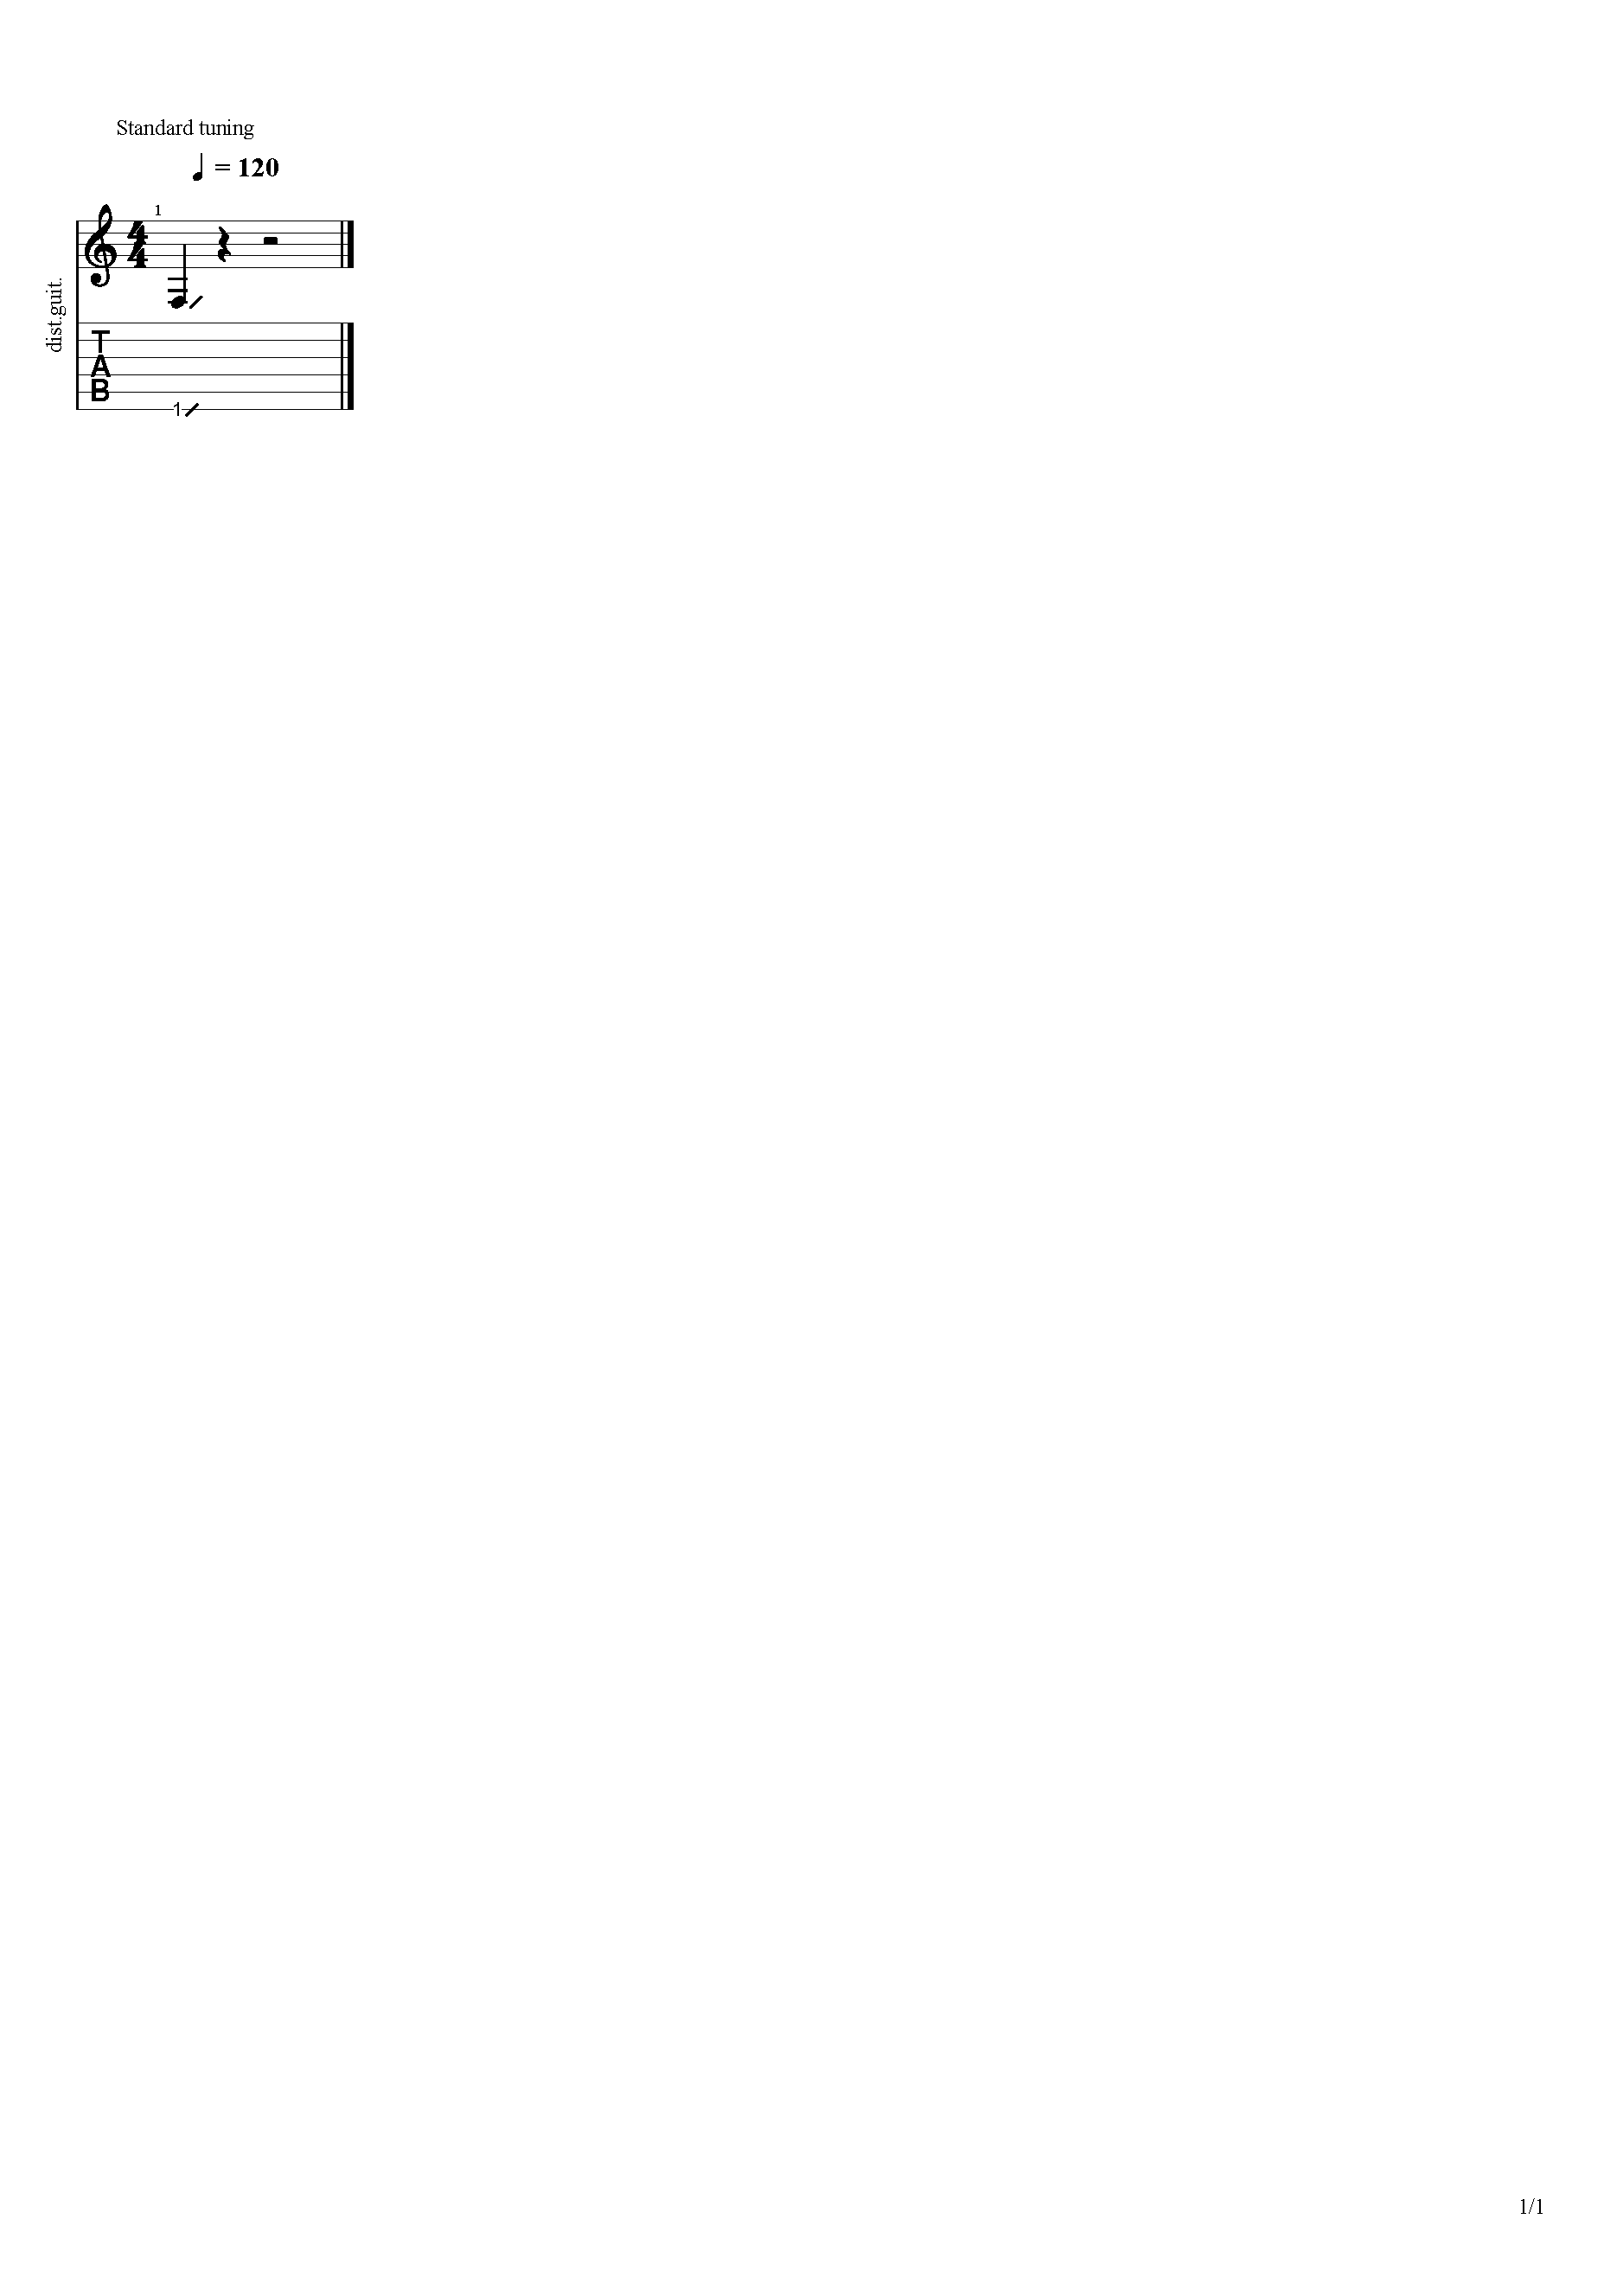
\includegraphics[trim={40 1040 690 100}, clip, width=0.16\linewidth]{slide_6.pdf}
\caption{Slide types}
  \label{fig:slide}
\end{figure}
\subsubsection{Dead note}
(muted note or ghost note)
Muting the string to produce a percussive sound.
\subsubsection{Hammer on / pull off}
Allows playing 2 notes in succession without picking the second note. Pressing down onto a higher fret to play a note without picking it, producing smooth legato transition between notes. 
Pulling off a higher fretted note while the lower fret note is still pressed.
\subsubsection{Vibrato}
Repeated bending and releasing a note to create subtle pitch variation
\subsubsection{Harmonic - Natural}
Producing bell-like, chime sound by lightly touching a string at specific points along the fretboard. 
\begin{figure}[htbp]
  \centering
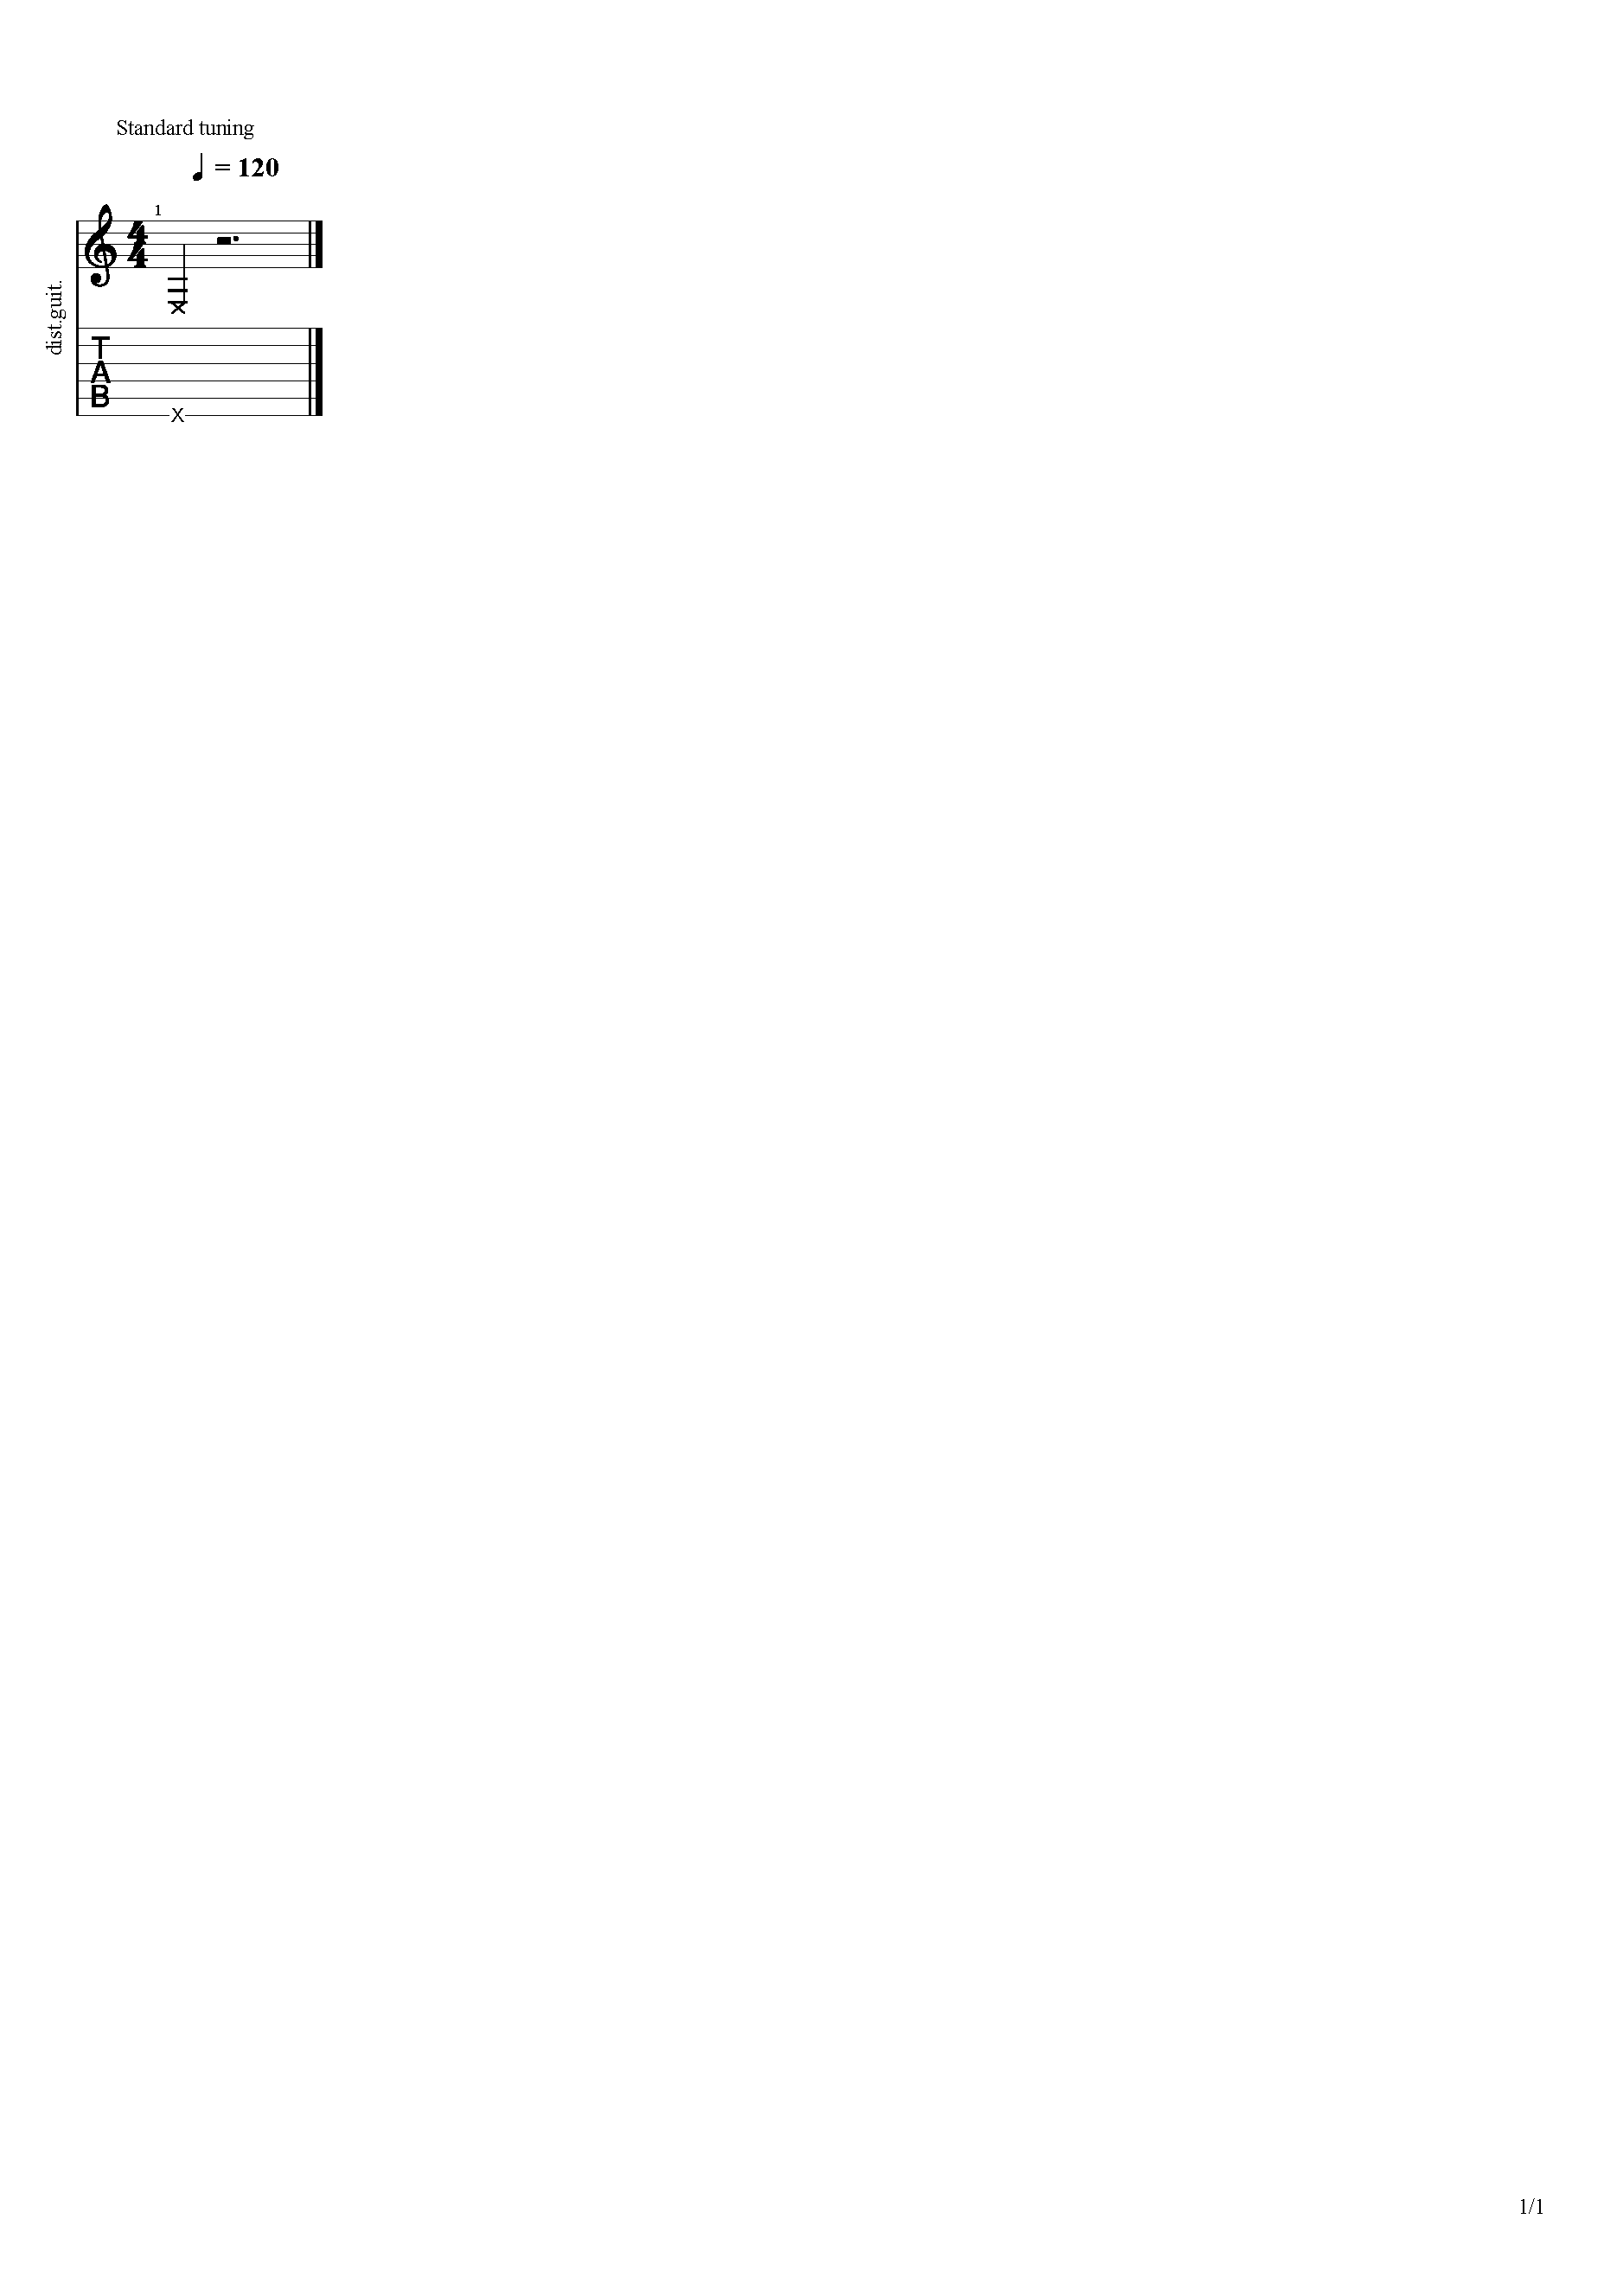
\includegraphics[trim={40 1040 690 100}, clip, width=0.22\linewidth]{dead.pdf}
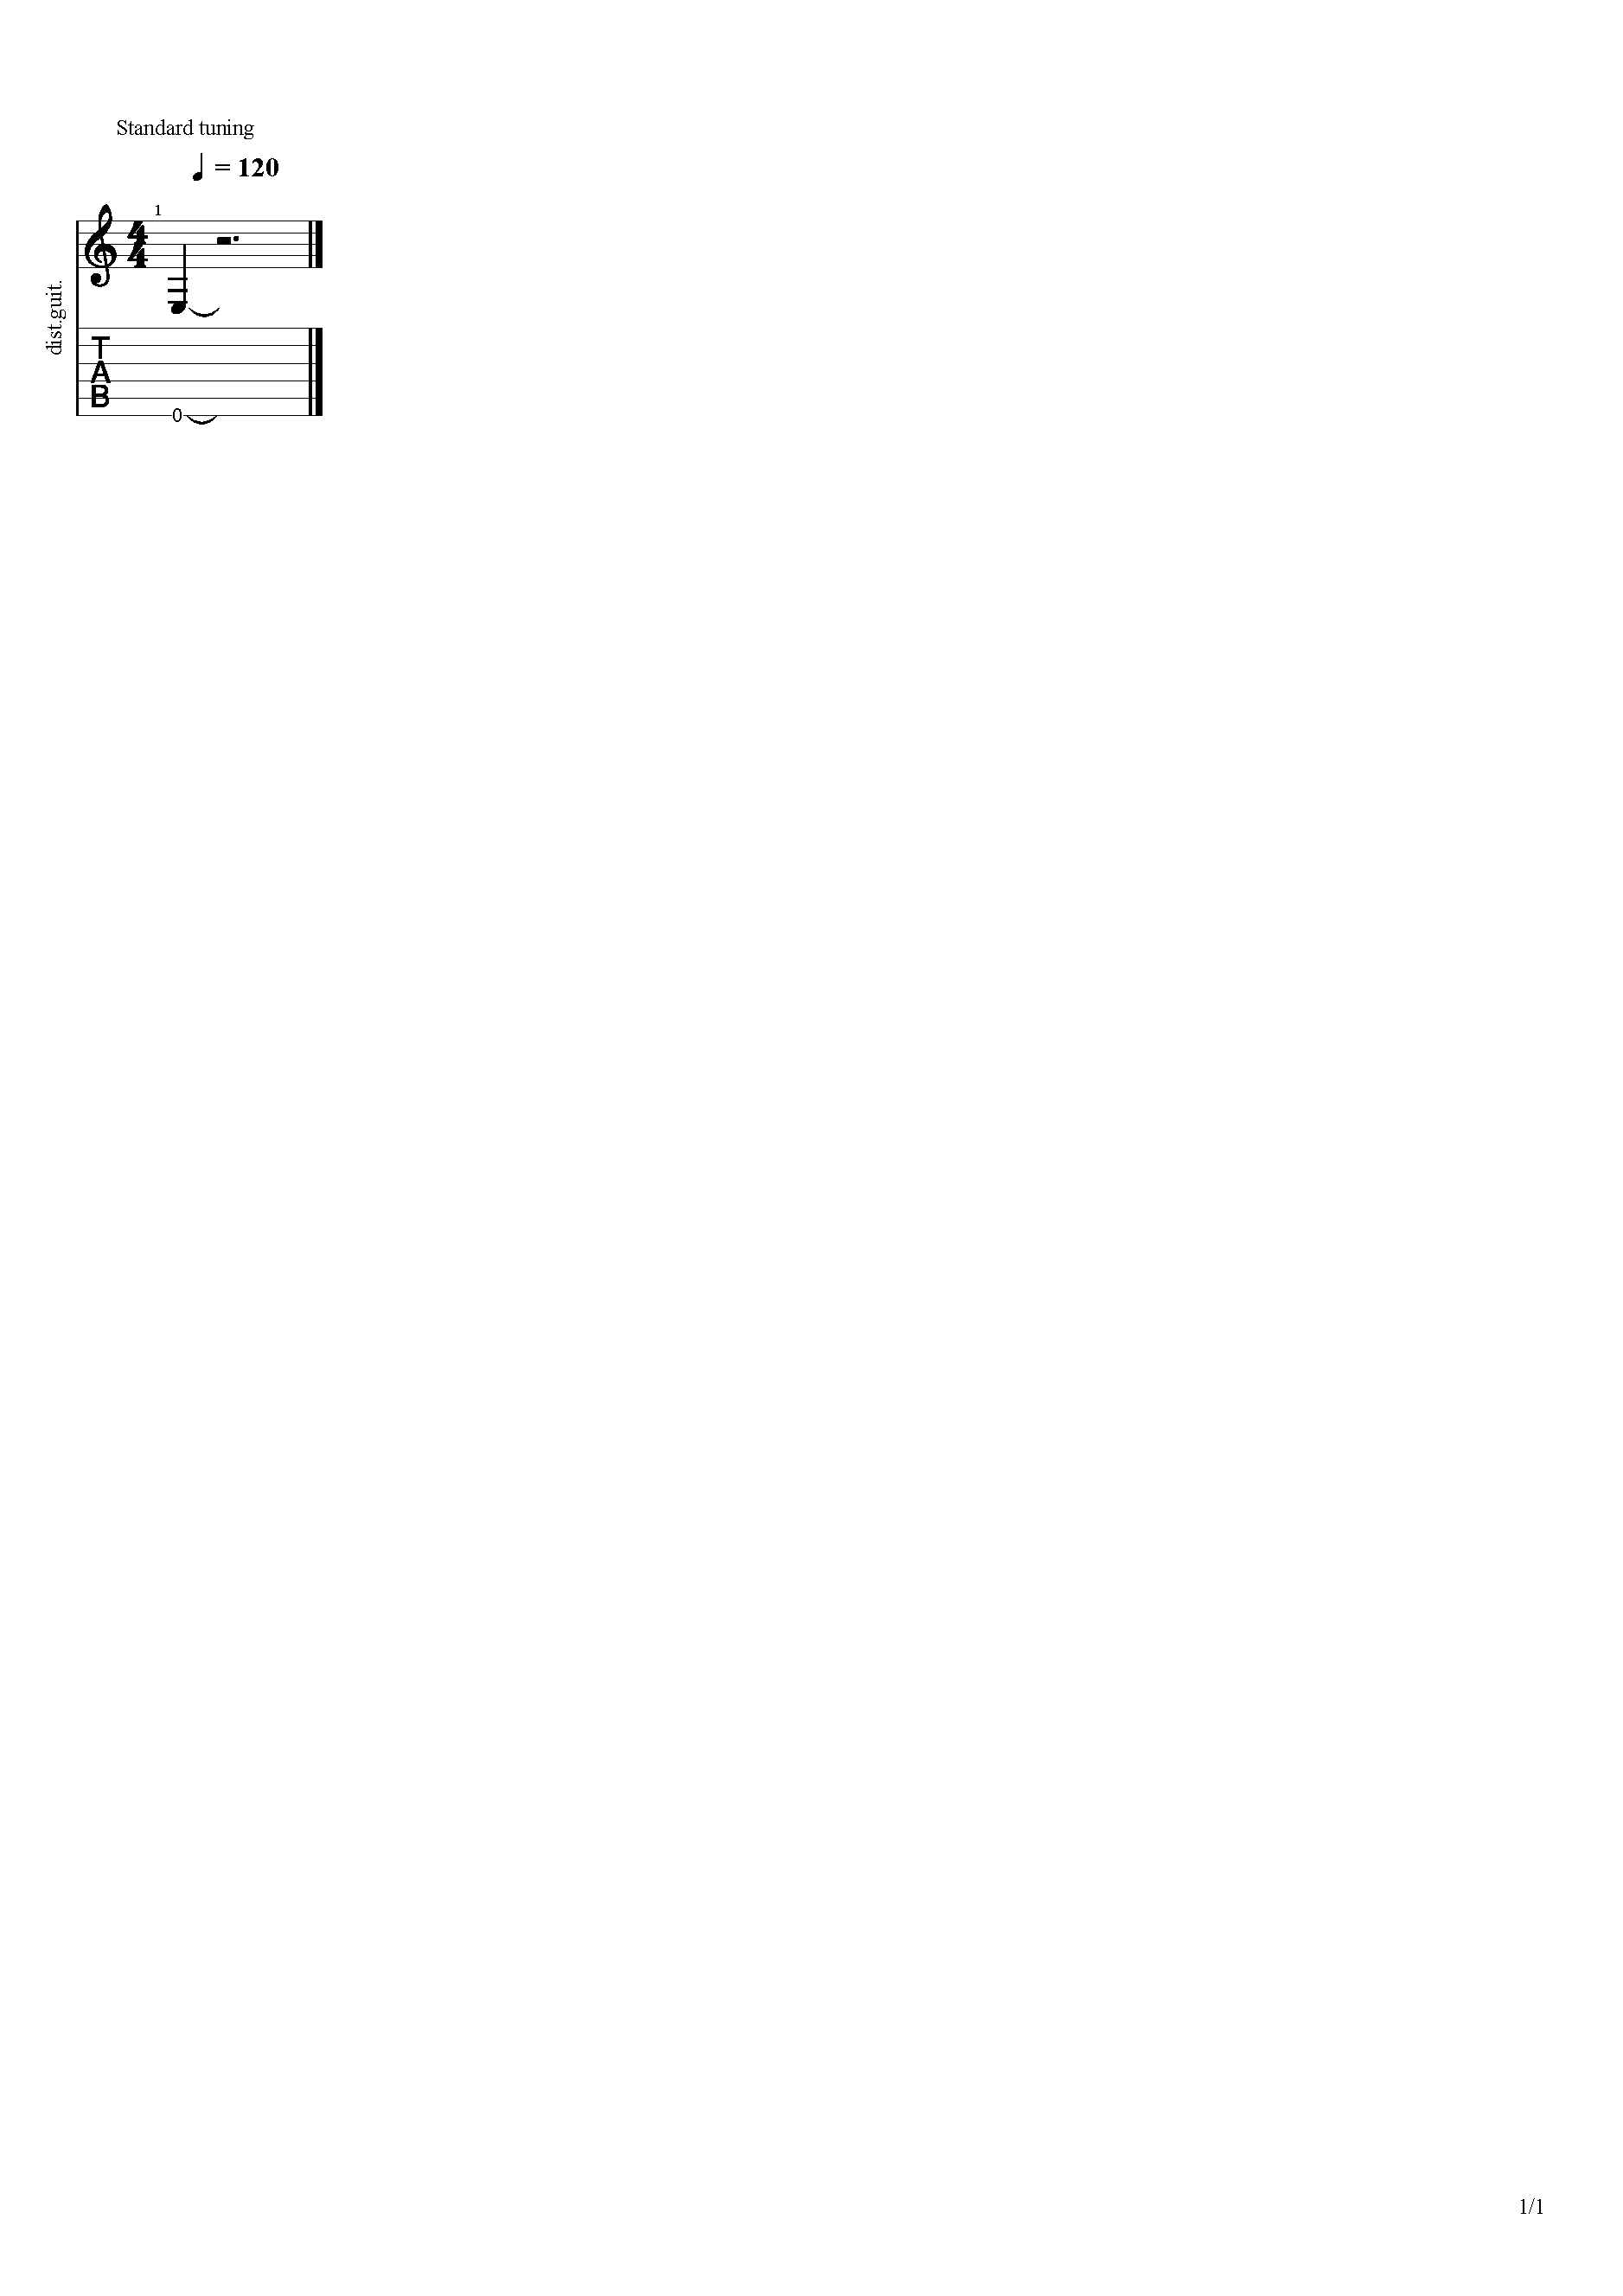
\includegraphics[trim={40 1030 690 100}, clip, width=0.22\linewidth]{hammer.pdf}
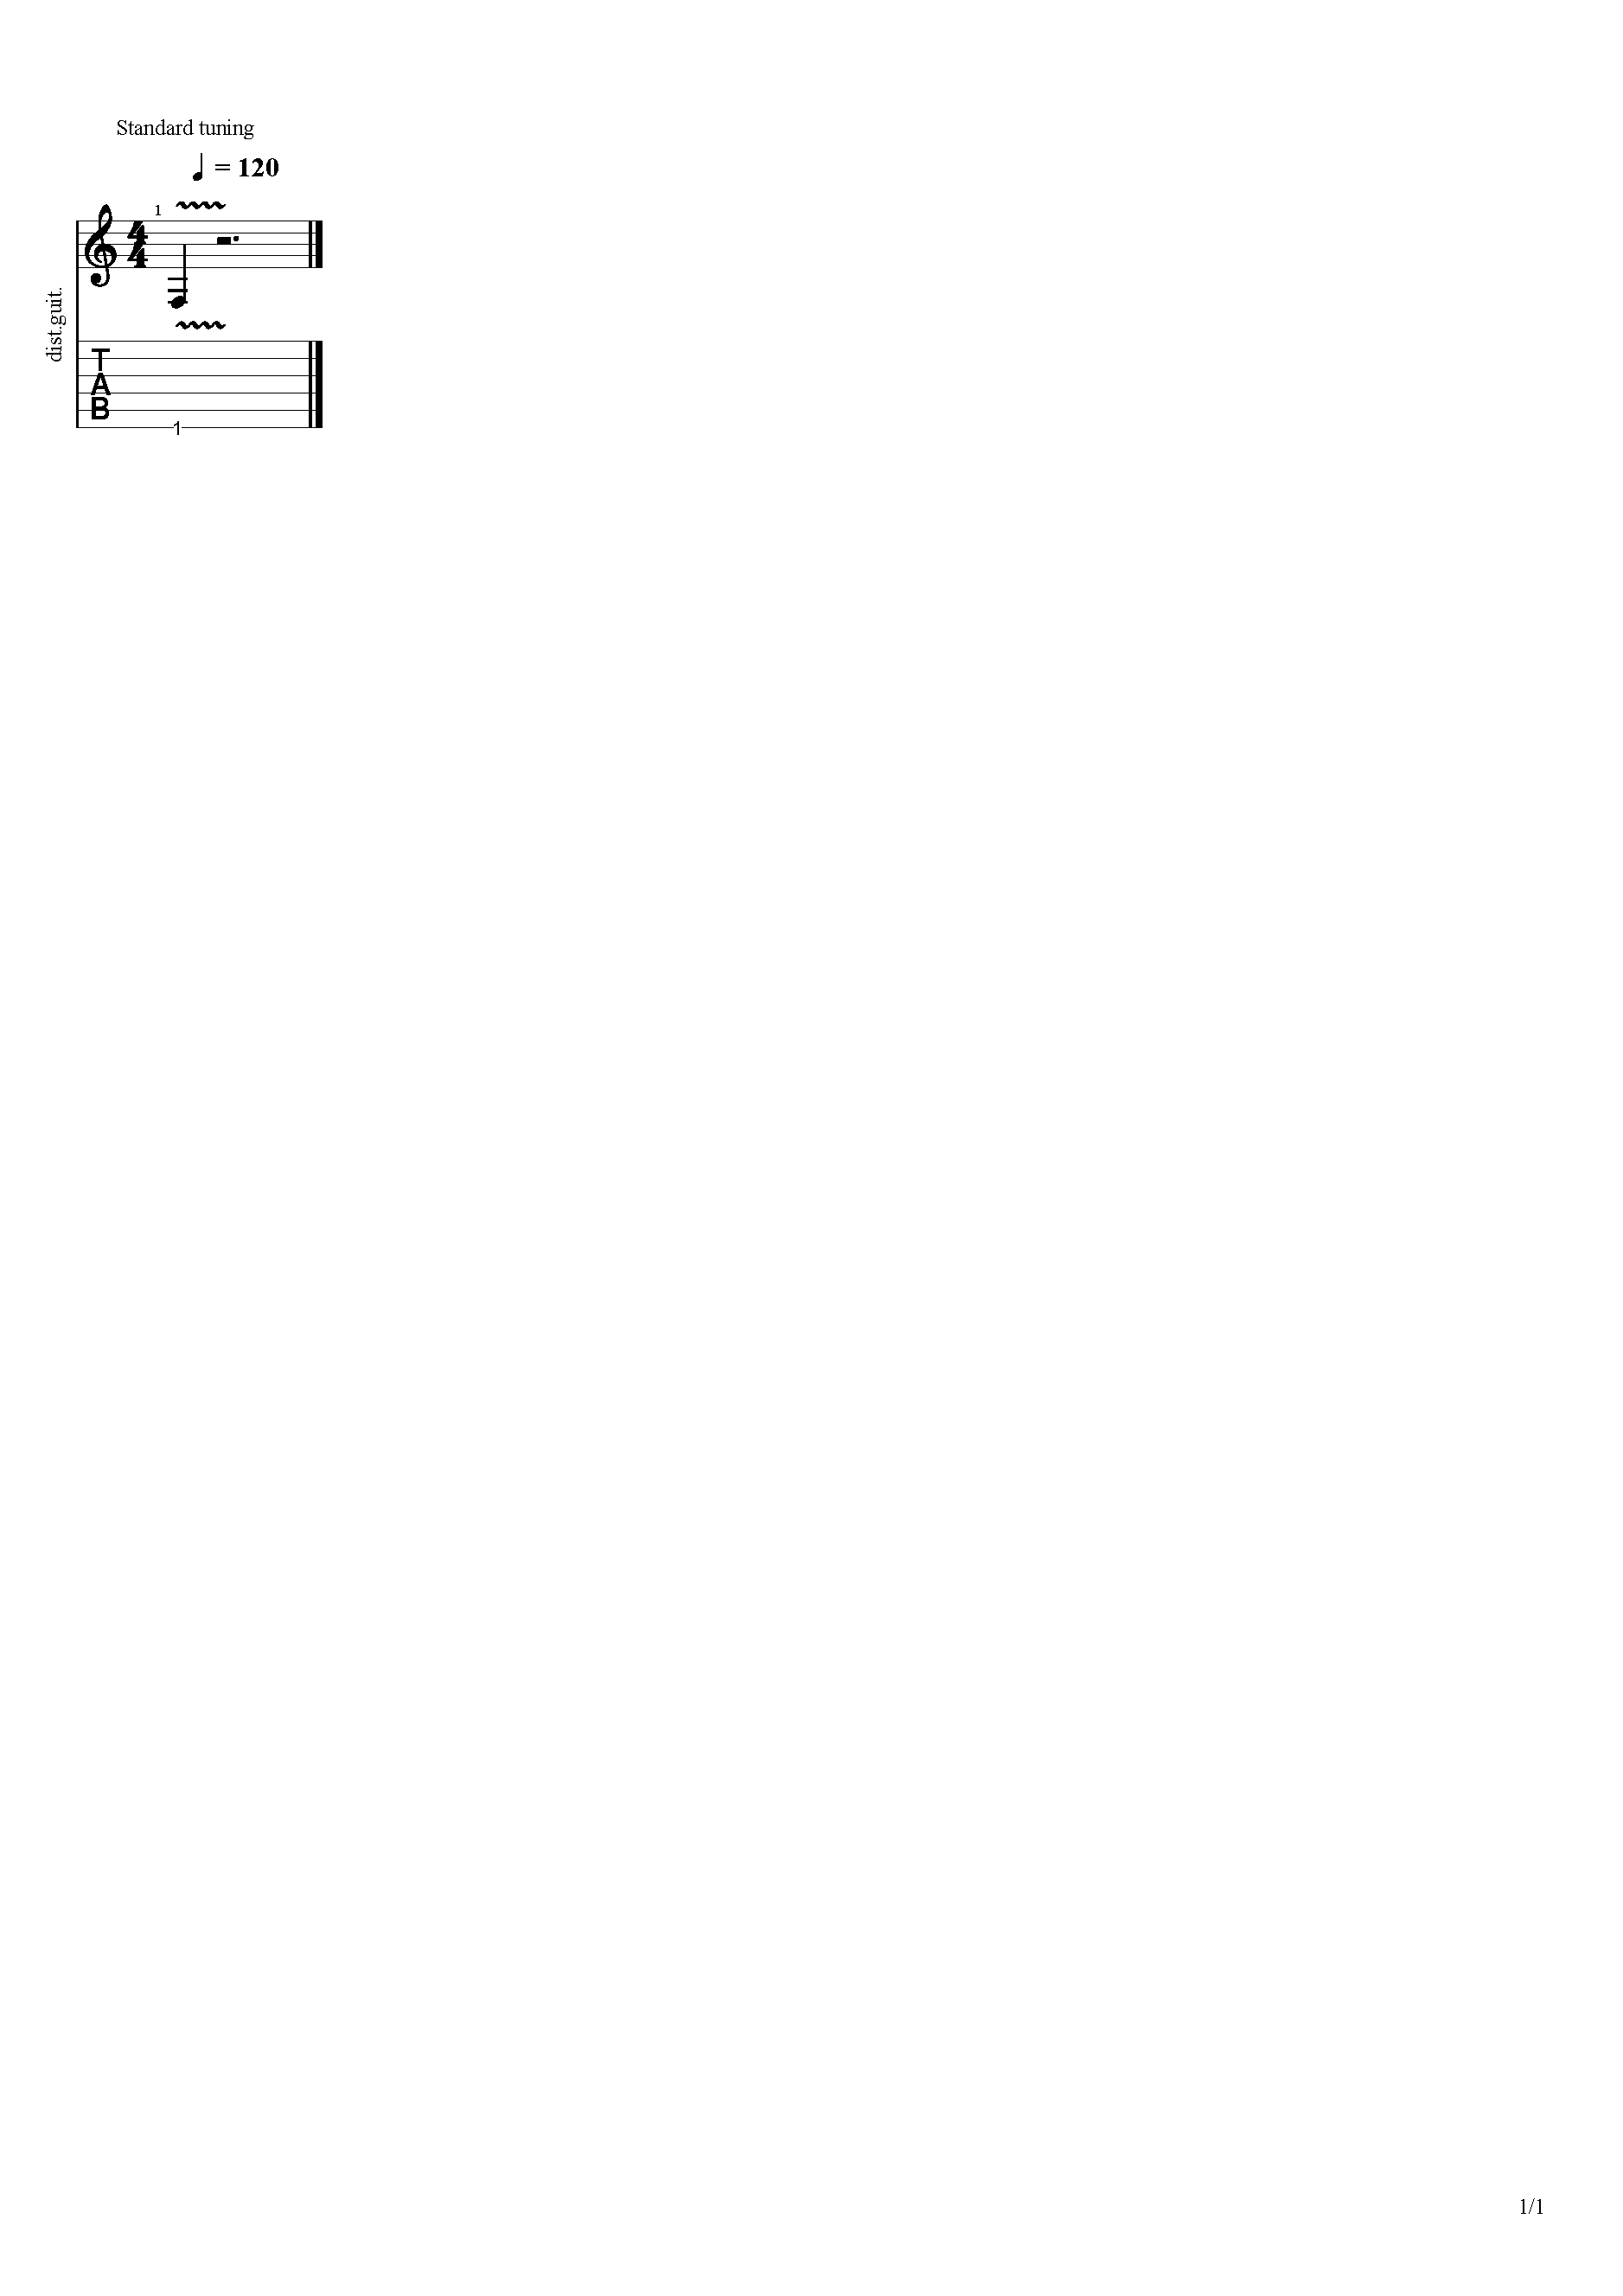
\includegraphics[trim={40 1020 690 100}, clip, width=0.22\linewidth]{vibrato.pdf}
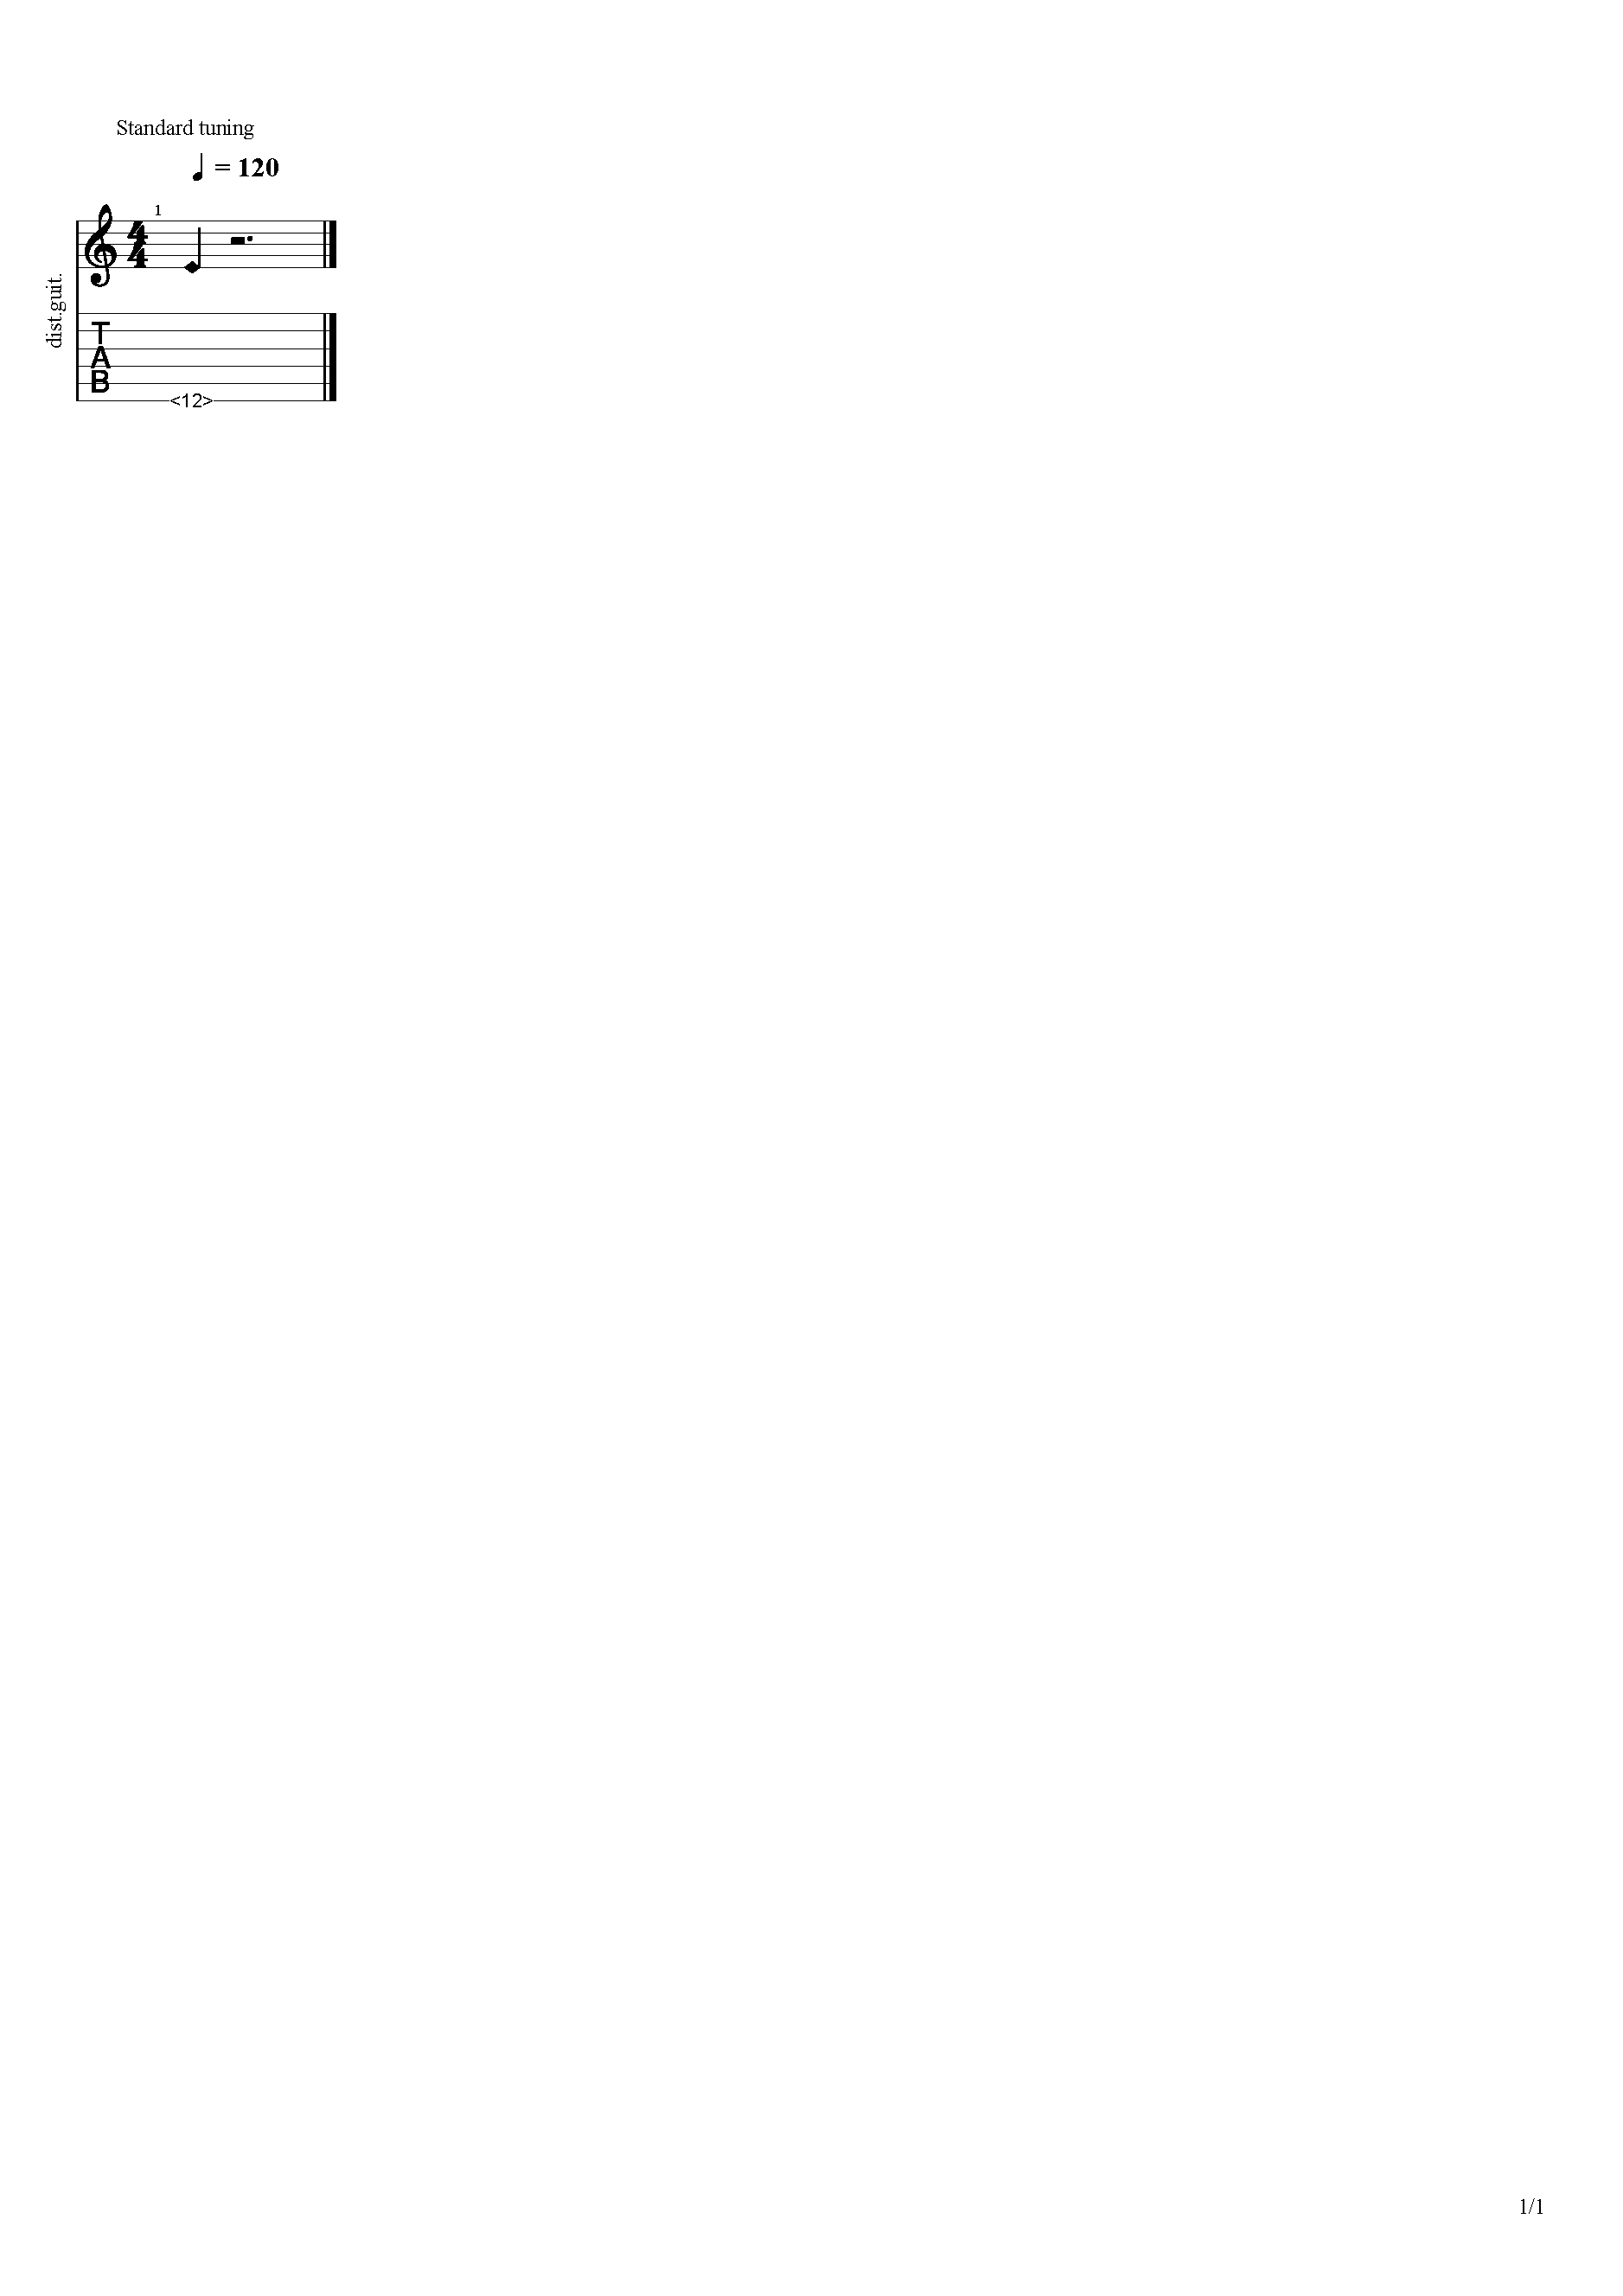
\includegraphics[trim={40 1040 710 100}, clip, width=0.22\linewidth]{harmonic_1.pdf}
\caption{Dead note, Hammer On, Vibrato, Natural Harmonic}
  \label{fig:harmonic}
\end{figure}
\section{Statistics}

\acks{All acknowledgements go at the end of the paper before appendices and references.
Moreover, you are required to declare funding (financial activities supporting the
submitted work) and competing interests (related financial activities outside the submitted work).
More information about this disclosure can be found on the JMLR website.}


% Manual newpage inserted to improve layout of sample file - not
% needed in general before appendices/bibliography.

\newpage

\appendix
\section{}
\label{app:theorem}

% Note: in this sample, the section number is hard-coded in. Following
% proper LaTeX conventions, it should properly be coded as a reference:

%In this appendix we prove the following theorem from
%Section~\ref{sec:textree-generalization}:

In this appendix we prove the following theorem from
Section~6.2:

\noindent
{\bf Theorem} {\it Let $u,v,w$ be discrete variables such that $v, w$ do
not co-occur with $u$ (i.e., $u\neq0\;\Rightarrow \;v=w=0$ in a given
dataset $\dataset$). Let $N_{v0},N_{w0}$ be the number of data points for
which $v=0, w=0$ respectively, and let $I_{uv},I_{uw}$ be the
respective empirical mutual information values based on the sample
$\dataset$. Then
\[
	N_{v0} \;>\; N_{w0}\;\;\Rightarrow\;\;I_{uv} \;\leq\;I_{uw}
\]
with equality only if $u$ is identically 0.} \hfill\BlackBox

\section{}

\noindent
{\bf Proof}. We use the notation:
\[
P_v(i) \;=\;\frac{N_v^i}{N},\;\;\;i \neq 0;\;\;\;
P_{v0}\;\equiv\;P_v(0)\; = \;1 - \sum_{i\neq 0}P_v(i).
\]
These values represent the (empirical) probabilities of $v$
taking value $i\neq 0$ and 0 respectively.  Entropies will be denoted
by $H$. We aim to show that $\fracpartial{I_{uv}}{P_{v0}} < 0$....\\

{\noindent \em Remainder omitted in this sample. See http://www.jmlr.org/papers/ for full paper.}


\vskip 0.2in
\bibliography{SCORESET}

\end{document}
